%%%%%%%%%%%%%%%%%%%%%%%%%%%%%%%%%%%%%%%%%%%%%%%%%%%%%%%%%%%%%%%%%%% 
%                                                                 %
%                            ROOT FILE                            %
%                                                                 %
%%%%%%%%%%%%%%%%%%%%%%%%%%%%%%%%%%%%%%%%%%%%%%%%%%%%%%%%%%%%%%%%%%% 
%
%  Run LaTeX or pdfLaTeX on this file to produce your thesis.
%  To produce the abstract title page followed by the abstract,
%  see the file abstitle-phd.tex or abstitle-mas.tex.
%
%%%%%%%%%%%%%%%%%%%%%%%%%%%%%%%%%%%%%%%%%%%%%%%%%%%%%%%%%%%%%%%%%%%

% arara: pdflatex
% arara: bibtex
% arara: pdflatex
% arara: pdflatex

\documentclass[chap]{thesis}

% Use the first command below if you want captions over 1 line indented. A side
% effect of this is to remove the use of bold for captions (thesis default).
% To restore bold, also include the second line below.
\usepackage[hang]{caption}      % to indent subsequent lines of captions
\usepackage{graphicx}
\renewcommand{\captionfont}{\bfseries} % bold caption (needed with caption 
                                       % package to restore boldface.)
%\includeonly{rpichap1}  % use \includeonly to process only
                         % the file(s) listed inside the braces        
\newcommand{\comment}[1]{\textbf{Linyun: #1}}
%\newcommand{\comment}[1]{\ } % used to hide all comments
\begin{document}

%\include{rpititle-mas}   % titlepage material for Master's thesis or project
%%%%%%%%%%%%%%%%%%%%%%%%%%%%%%%%%%%%%%%%%%%%%%%%%%%%%%%%%%%%%%%%%%% 
%                                                                 %
%                            TITLE PAGE                           %
%                            PhD Thesis                           %
%                                                                 %
%%%%%%%%%%%%%%%%%%%%%%%%%%%%%%%%%%%%%%%%%%%%%%%%%%%%%%%%%%%%%%%%%%% 
%  This file produces the title page, copyright page (if requested)
%  and the Table of Contents, List of Figures and List of Tables.
% 
%  To produce the abstract title page followed by the abstract,
%  see the template file, "abstitle-phd.tex"
%%%%%%%%%%%%%%%%%%%%%%%%%%%%%%%%%%%%%%%%%%%%%%%%%%%%%%%%%%%%%%%%%%%
    
% Supply information for use on title page:
%   
\thesistitle{\bf Automatic Provenance Capturing for Research Publications}
\author{Linyun Fu}
\degree{Doctor of Philosophy}
\department{Computer Science} % provide your area of study here; e.g.,
%  "Mechanical Engineering", "Nuclear Engineering", "Physics", etc.

\signaturelines{4}     %max number of signature lines is 7        
\thadviser{Peter Fox}
 %\cothadviser{Second Adviser} % If you have 2 thesis advisers
\memberone{Deborah McGuinness}        
\membertwo{Francine Berman}        
\memberthree{Heidi Newberg}
%\memberfour{Marcus Aurelius} % must change signaturelines to 5 if using this 5 members
%\memberfive{Marcus Junius Brutus} % must change signaturelines to 6 if using this 6 members
%\membersix{Nikola Tesla} % must change signaturelines to 7 if using this 7 members

\submitdate{November 2015\\(For Graduation December 2015)}        
%\copyrightyear{1685}   % if omitted, current year is used.        

% Print titlepage and other prefatory material:
%    
\titlepage     
\copyrightpage         % optional           
\tableofcontents        
\listoftables          % required if there are tables
\listoffigures         % required if there are figures


   % titlepage material for PhD thesis 
%%%%%%%%%%%%%%%%%%%%%%%%%%%%%%%%%%%%%%%%%%%%%%%%%%%%%%%%%%%%%%%%%%% 
%                                                                 %
%                         ACKNOWLEDGEMENT                         %
%                                                                 %
%%%%%%%%%%%%%%%%%%%%%%%%%%%%%%%%%%%%%%%%%%%%%%%%%%%%%%%%%%%%%%%%%%% 
 
\specialhead{ACKNOWLEDGMENT}

I would like to thank Peter Fox for his advise and encouragements throughout the process of the research presented in this thesis. I would also like to thank Xiaogang Ma for his contribution of time and insights as a domain scientist in the ontology design of PROV-PUB-O and the ontology usability evaluation method development.

I would also like to thank my wife, Wenyu Li, for her love and care and encouragements during the last two years. This work would be impossible without her company.

  % include for acknowledgements
%%%%%%%%%%%%%%%%%%%%%%%%%%%%%%%%%%%%%%%%%%%%%%%%%%%%%%%%%%%%%%%%%%% 
%                                                                 %
%                            ABSTRACT                             %
%                                                                 %
%%%%%%%%%%%%%%%%%%%%%%%%%%%%%%%%%%%%%%%%%%%%%%%%%%%%%%%%%%%%%%%%%%% 
 
\specialhead{ABSTRACT}
 
Provenance is critical for research publication readers to correctly interpret report content and enables them to evaluate the credibility of the reported results by digging into the software in use, source data and responsible agents. It also enables the readers to reproduce the scientific conclusions by changing the process leading to the reported results. However, creating proper provenance for research publications is very hard. First, it requires knowledge of proper provenance information to capture for the report creating process, causing either extra learning overhead on the domain scientists who write the reports or communication overhead between domain scientists and informatics experts who know how to keep track of the provenance. Second, since provenance information is usually closely related to the computational environment of the programs used during the process of preparing publications, it is often necessary to also capture the configurations of program running platform such as the operating system or even the computer hardware in order to get useful provenance information for the purpose of enabling publication readers to reproduce and validate the content, which requires knowledge of the computational system. This knowledge is usually outside the reach of both domain scientists and informatics experts, so they would depend on system administrators to get or learn by themselves the configuration related provenance information, causing more communication/learning burden. Third, it requires extra efforts to capture provenance on top of the authoring work, which already includes writing manuscripts, getting data from various sources, using various tools to process data and running programs to generate tables and figures, so the creation of provenance information is usually distracting to the authors and thus insufficiently motivated. 

Existing scientific workflow management systems such as VisTrails \cite{freire2014reproducibility}, Kepler \cite{ludascher2006scientific}, Taverna \cite{wolstencroft2013taverna} and ReproZip \cite{chirigati2013reprozip} do not provide satisfactory solutions to any of the three problems mentioned above. Users need to learn how to use these systems in order to create provenance information with them. Information for program running platforms either is not taken care of at all, or heavily depends on the specific system architecture, e.g., by tracking operating system calls, as in the case of the ReproZip system. These systems require their users to take the extra efforts of integrating the provenance into the workflow systems, and usually authors do not have enough incentive to do this job after writing the publications.

In this thesis, we propose a paradigm of preparing research publications to overcome all the problems associated with provenance capturing in the preparing process, which is to create publications with libraries that transparently capture the proper provenance information on a portable platform.



The proper provenance information to be captured is defined in an ontology designed to model the preparing process of research publications. Although there are workflow models developed for capturing provenance in computational experiments \cite{groth2006architecture, groth2009recording}, models for provenance in publication preparation are not found, so even if the authors are willing to take the pains to record the necessary provenance information and make it public, they may find themselves lost in the problem of \emph{what to record and how to encode}. The authoring process modeling ontology aims to tell the authors what is necessary for the reproducibility of their publications, and the recorded information can be readily encoded with the Resource Description Framework.
%Unlike models for computational experiments, the ontology presented in this thesis pays special attention to the human factor in the process, which is a significant feature of the publication preparing process compared with the computational experiment workflows. The provenance capturing mechanism is driven by the ontology.

A portable platform is a software package or a Web application that runs on some environment that is available on all the popular computational systems, such as a Java program which runs on the Java Virtual Machine, a Python program which runs with the Python interpreter, or a Web based application written in HTML, JavaScript and/or PHP scripts which runs on any of the mainstream Web browsers. Preparing research publications based entirely on a portable platform eliminates the necessity of capturing provenance information down to the computer system level. Two desirable features for the platform are that 1) it should supply all the functions needed in creating research publications, and 2) these functions can be used in a way that is similar to the software packages the author is used to working with. To ensure the first feature, the platform needs to be extensible, better if it already has a strong development community to supply a plethora of evolving modules. The second feature requires that the platform supports popular interactive editing modes widely accepted in the research community. Examples include those seen in research software packages such as MATLAB and R.

Transparent provenance capturing means the authors using the platform are not exposed to the provenance information model that drives the capturing mechanism, which is triggered each time a publication preparing action is taken, e.g., when a block of manuscript is written, when some data are downloaded from an external source, or when a plot is created by calling a library function with the downloaded data. Capturing provenance information in this way eliminates the need to ask the authors to explicitly input provenance information. It also removes from the authors the burden of learning what provenance information to capture or communicating with people who are familiar with provenance capturing.

Contributions of the work in this thesis are 1) the creation of an ontology for capturing provenance in the process of research publication preparation; 2) the specification of a provenance capturing mechanism driven by the ontology. The mechanism makes the provenance capturing actions transparent to the authors of research publications; and 3) the implementation of a provenance aware publication preparing platform prototype that fulfills the requirements posed by the specified provenance capturing mechanism.

%We originally planned to cover all the three aspects mentioned above in this proposal, but while we investigated the first one, i.e., the ontology for capturing provenance during publication preparation, we found that the evaluation of such an ontology is itself an interesting and big research topic, so this proposal will focus on this first aspect.
%\comment{A library that transparently captures provenance information enables researchers to focus on the science part of creating publications, without being distracted by the provenance preserving part. As long as the functions provided by the library are invoked how to ensure functionalities active development community}
%
%\comment{Typical activities include importing a library to the workspace, calling a function to get source data or to create an image, adding a text block to the publication, and rerunning a code block with a different set of parameters.}
%
%\comment{The challenges, existing efforts and their shortcomings will be written here.}
%
%\comment{Feasibility comes here.}
%
%\comment{Contributions come here.}
 % abstract
\chapter{INTRODUCTION}
\label{introduction}
\section{What does provenance mean in this thesis}
According to Oxford English Dictionary, provenance is the chronology of the ownership, custody or 
location of a historical object. For digital artifacts, the Provenance Working Group of World Wide 
Web Consortium (W3C) defined provenance as \begin{quote}\textit{information about entities, activities, and 
people involved in producing a piece of data or thing, which can be used to form assessments about 
its quality, reliability or trustworthiness.}\end{quote} This thesis focuses on provenance for 
research publications, which are a kind of digital artifact, so in this thesis, the word 
\emph{provenance} means information about data, their stewardship activities, and agents involved in the 
production of results reported in research publications. Here \emph{data} may come from observations, 
model runs or repositories supporting data reuse; \emph{data stewardship activities} include semantical, 
syntactical and physical changes of data; \emph{agents} are people, organizations and software agents 
relevant to the data and their stewardship activities at any phase of the data lifecycle; \emph{results} 
are a special kind of objects derived from data that are the final products reported in research publications. Note that this definition 
of results deviates from the concept of \emph{scientific conclusions}, which are the insights the results try to support and thus are hard to model. Also note that information about the \emph{linkage} among these data, activities and agents are also implicitly included in provenance. For example, the fact of a data object \emph{being generated by} an activity could be captured as a link between the data object and the activity. Such linkage information is one of the major differences between provenance and separate descriptive metadata chunks.

Semantical changes of data mean the changes in the actual meaning of data, which is a combination of the content and the context. Looking at content or context alone may lead to wrong judgment about whether a piece of data have been semantically changed. For example, a number ``1'' changed to ``1000'' may not have been semantically changed because the former number represents quantity in kilogram and the latter in gram and thus the meaning of the number has not changed. It is a syntactical change instead.

Syntactical changes of data mean the changes in the structure of data. A typical example is changing 
data serialized in XML to JSON without changing the actual meaning of the data. This is especially important in Web-based usage as the transmission mechanisms, that is, serialization, requires conversion to a different structure.

Physical changes of data mean changes in locations, character encodings and accessibility of data. 
For example, data downloaded from an online source are the result of changing the locations of the 
original data (now they are in two places). When the location of a piece of textual data changes, the 
character encoding might change as well if the source and target storages follow different encoding 
schemes. Changes of data sharing permissions are a kind of physical changes that change the 
accessibility of data. 

This classification of changes of data is based on the semiotic framework proposed by Burton-Jones et al. See Table 2 in \cite{burton2005semiotic}.

All these changes are performed by agents, mostly software agents such as software tools, programs 
using library functions and command line scripts, through running software in command line, GUI or 
interactive mode, function invocations, and script running.

Information about people and organization agents tells the readers who owns, is responsible for, or 
should get credit for the publication and the data and software it used, which makes it possible to 
recognize and reward not only the publication authors, but also data and software producers. 
Recognition of these people or organizations benefits all researchers with better data and software 
\cite{parsons2010data, goble2014better}.

Useful information about software agents, other than their owners, responsible parties and 
contributors, falls into two categories. The first one is static information such as source code and 
documentation. This kind of information is needed for readers of the publications to understand and 
reuse the software to \emph{reproduce} the scientific conclusions. The second category of software 
agent information is dynamic information, i.e., information associated with activities these agents 
perform. Examples include their running environments such as library dependencies and system 
environment variable values, and configurations such as parameters and command line arguments, at 
each time they run, and the communication history of a certain interactive programming session. Such 
information plays an important role in \emph{replicating} computational experiments.

Note that the two words \emph{reproduce} and \emph{replicate} are used carefully here, whose meanings 
will be discussed in detail in the next section.


\section{Why is provenance important in scientific works}
With sufficiently rich provenance information, a piece of scientific work would have the following two 
desirable features, namely \emph{transparency} and \emph{reproducibility}. At the very basic level, 
provenance helps answer questions such as \emph{``What data are the reported results based on, and 
where does this piece of data come from''}, \emph{``Have the data been modified, in what ways''} 
\cite{davidson2008provenance}, which makes a piece of scientific work \emph{transparent}, meaning the 
readers have access to the knowledge of the data, their stewardship activities and associated agents. 
With richer provenance on data stewardship activities and software agents, readers have the ability to 
perform the same experiments carried out by the authors, making the work \emph{replicable}, meaning 
the same experiment can be carried out in a different lab, according to Goble's keynote presentation 
at ISMB/ECCB 2013. The final goal of provenance is to enable readers to carry out different 
experiments to validate the same scientific conclusion that the original experiment tries to justify, 
which is, according to \cite{drummond2009replicability}, \emph{reproducibility}.

The first feature, transparency, not only increases the trustworthiness of the scientific work by 
making the research process leading to the publication open to public scrutiny, but also reveals the 
work that would otherwise not be recognized, such as the development, configuration, integration and 
deployment of software for experiments \cite{goble2014better}.

Here \emph{replicability} and \emph{reproducibility} are defined as in 
\cite{drummond2009replicability}. In the last decade, the word \emph{reproducibility} pops up a lot 
in discussions about provenance. For example, 
%Altintas et al., in \cite{altintas2004kepler}, claims that scientific research is generally held to be of good provenance when it is documented in detail sufficient to allow reproducibility, and 
Boose et al., in \cite{boose2007ensuring}, pointed out that
\begin{quote}\emph{data sets are reliable when the process used to create them are reproducible and 
analyzable for defects.}\end{quote}
Drummond pointed out in \cite{drummond2009replicability} that \emph{reproducibility} in the sense of 
carrying out the same experiments by different researchers should actually be called 
\emph{replicability}.

Schwab et al. in \cite{schwab2000making} argue that the readers can usually identify the parameter 
they want to modify, the input data that they want to exchange, or the source code that they want to 
inspect after analyzing the execution of the original experiment. Based on this argument, we believe 
that replications of experiments help readers to do different experiments. In fact, exact replication 
is impossible since the times of performing experiments must differ, so we treat replication as a 
special case of reproduction where readers perform really similar experiments as the original one the 
authors did.

In other words, reproducibility can be viewed as a spectrum of readers' increasing ability to perform 
more and more different experiments from the original one. Here is an example of a list of actions 
readers can take based on the original experiments, in the ascending order of reproducibility:
\begin{itemize}
\item parameter tuning
\item change of function application order
\item introduction of new functions
\item use of new source data
\item use of new scientific approach
\end{itemize}
We can see that provenance of the original experiment supports all these actions by providing the 
static and dynamic information of the software agents involved and the data used.
% \comment{treat replicability as a special case of reproducibility}
% from 2014-10-20-computational-vs-scientific-reproducibility.txt


% how difficult and anti-motivated its capturing is to the authors, stating the authoring workflow here. Say that currently authors lack both the ability and the motivation to capture provenance for their publications, given the currently available tools. 
\subsection{Pervasiveness of computational methods and lack of transparency in them}
Table~\ref{table:jasa} shows how many articles in June issues of Journal of the American Statistical Association (JASA), the flagship journal for statistical research in the United States, used computational methods, as well as how many of them made their code publicly available.
\begin{table}
	\centering
	\caption[Computational methods and code availability of JASA]{Number of articles using computational methods and their code availability in June issues of Journal of the American Statistical Association in 1996, 2006, 2009 and 2011. Courtesy Victoria Stodden.}
	\label{table:jasa}
	\begin{tabular}{r|cc}
		JASA June & Computational Articles & Code Publicly Available \\ 
		\hline 1996 & 9 of 20 & 0\% \\ 
		 2006 & 33 of 35 & 9\% \\ 
		 2009 & 32 of 32 & 16\% \\ 
		 2011 & 29 of 29 & 21\% \\  
	\end{tabular} 
\end{table}
We can see from the table that using computational methods is the trend. Virtually every article published at JASA in the past 5 years uses computational methods, but very few of them are exposing code to the public.
In her talk in 2011 \cite{stodden2011establishing}, the author argued that the lack of transparency is hurting the credibility of scientific research.

In the area of biomedical research, Bustin in \cite{bustin2015reproducibility} pointed out that there is increasing concern about the reliability of biomedical research, and a comment article plus a series of five articles published in the Lancet journal in early 2014 suggested that up to 85\% of research funding is wasted in unreliable research. The comment article introduces the series and discusses the consistent and colossal failure of initially promising research findings to translate into improvements in health care because of the many economic, political, social and cultural factors that influence researchers, funders, regulators, institutions and companies \cite{macleod2014biomedical}. 
%The first article in the series pointed out that the research studies supported by around US\$240 billion worldwide investment may have problems at the time funders decide what research to support, causing that much research does not lead to worthwhile achievements and that good research ideas do not yield the anticipated results \cite{chalmers2014increase}. 
The second article in the series highlights that an absence of detailed written protocols and poor documentation of
research is common and that inadequate emphasis is placed on recording of research decisions and on reproducibility of research \cite{ioannidis2014increasing}. 
%The third article discusses the modern approach to the regulation, governance, and management of biomedical research and emphasizes how inefficient management can easily compromise the interests of patients and the public \cite{salman2014increasing}. 
The fourth article points out that a large percentage of protocols, reports and datasets associated with health research are rarely available, and there is selective reporting of methods and results, which leads to the introduction of bias and wastes huge amounts of research funding \cite{chan2014increasing}. The final article reemphasizes the absolute requirements for accurate, exhaustive and transparent reporting and notes that although reporting guidelines are important, they are all much less adopted and adhered to than they should be \cite{glasziou2014reducing}. The editors of the series make the revolutionary suggestion that rather than using journal impact factors to assess academics, it might be more reasonable to judge the researchers' work with the rigorousness of methodology, the transparency of reporting and the reproducibility of results, which would of course facilitate the publication of more reliable and biologically relevant data.

Stodden in \cite{stodden2014enabling} pointed out that digital scholarly objects such as data and code have become essential for the effective communication of computational findings. Computations are frequently of such a complexity that an explanation sufficiently detailed to enable others to replicate the results is not possible in a typical scientific publication. A solution to this problem is to accompany the publication with the code and data that generated the results and communicate a \emph{research compendium} \cite{gentleman2007statistical}. However, the scientific community has not yet reached a stage where the communication of research compendiums is standard \cite{donoho2009reproducible}. A number of delicate regulatory and policy changes are essential to catalyze both scientific advancement and the development of applications and discoveries outside academia by making the data and code associated with scientific discoveries broadly available.

%\comment{review Gentleman 2007 and Donoho 2009}

The earliest work on research reproducibility we have found so far is in the after dinner talk by Jon Claerbout at National Research Council meeting on High Performance Computing in Seismology on October 2nd, 1994\footnote{Seventeen years of super computing and other problems in seismology. Available at http://sepwww.stanford.edu/sep/jon/nrc.html. Accessed on May 10th, 2015.}, where Claerbout stated his famous slogan ``in engineering, a published paper is an advertisement of scholarship'', which Buckheit and Donoho later paraphrased as 
\begin{quote}\emph{
	An article about computational science in a scientific publication is \emph{not} the
	scholarship itself, it is merely \emph{advertising} of the scholarship. The actual scholarship is the 
	complete software development environment and the complete set
	of instructions which generated the figures.}
\end{quote}
in \cite{buckheit1995wavelab}, where they talked about why and how they
made their wavelet analysis MATLAB routines, namely WaveLab, publicly available as a humble step towards really reproducible research, and pointed out that
\begin{quote}\emph{
	to work in accordance with this goal, we must decide on a discipline
	of how we will structure our computational experiments. We must also then proselytize
	among others in our group to get them to adopt this discipline.}
\end{quote}
Two decades have passed, ``this discipline'' seems still hindering the authors from recording the details of their computational experiments in such a manner that others can readily replicate their work.

\section{Why is it hard for the authors to record provenance}
The reasons include subjective and objective. On the subjective side, authors may consider the details of computational experiments non-essential to their work. They want readers to be inspired by their ideas instead of paying unnecessary attention to the details of the source code, but actually the additional materials in the form of source code and datasets rarely harm the readers by distracting them to minor details. On the objective side, recording provenance can be distracting and counter-productive to the authors due to its easy-to-miss characteristics as well as its diverse spatial and temporal distributions. This thesis will focus on alleviating the difficulty on this side.

It is a fallacy that the authors do not have the knowledge of everything happened during the process 
of the research work. The fact that they successfully got the reported results proves that they 
actually have, at certain times, all the knowledge of provenance that is sufficient for the 
replication of their work. Some pieces of the provenance are just so transient that if they do not 
get recorded at the right time, they get lost forever.

We will use the creation of a tabular summary of a dataset as our running example. Authors first use some 
download software package such as \emph{GNU Wget}\footnote{GNU Wget: https://www.gnu.org/software/wget/, accessed on November 24th, 2015.} to download the dataset from a certain place online, and then 
use some data analysis software package to generate meaningful data products from the dataset, 
followed by creating the summary table with some table making software package. During this process 
of table creation, we recognize more or less the following provenance pieces.
\begin{itemize}
\item What download software package was used, including its name, distribution and version.
\item Where the dataset was downloaded, including its URL.
\item When the dataset downloading activity started and ended.
\item Who executed the downloading operation.
\item The information about the data analysis software package used, including its API documentation.
\item The information about the data analysis operations performed, including functions called along 
with their argument values, and parameter values used. 
\item The time period of the data analysis activity.
\item Who analyzed the dataset.
\item The information about the table making software package.
\item The time period of making the summary table.
\item Who created the table.
\end{itemize}
Figure~\ref{prov-pieces} illustrates how these pieces of provenance information scatter all over the 
creation process of the summary table.
\begin{figure}
\centering
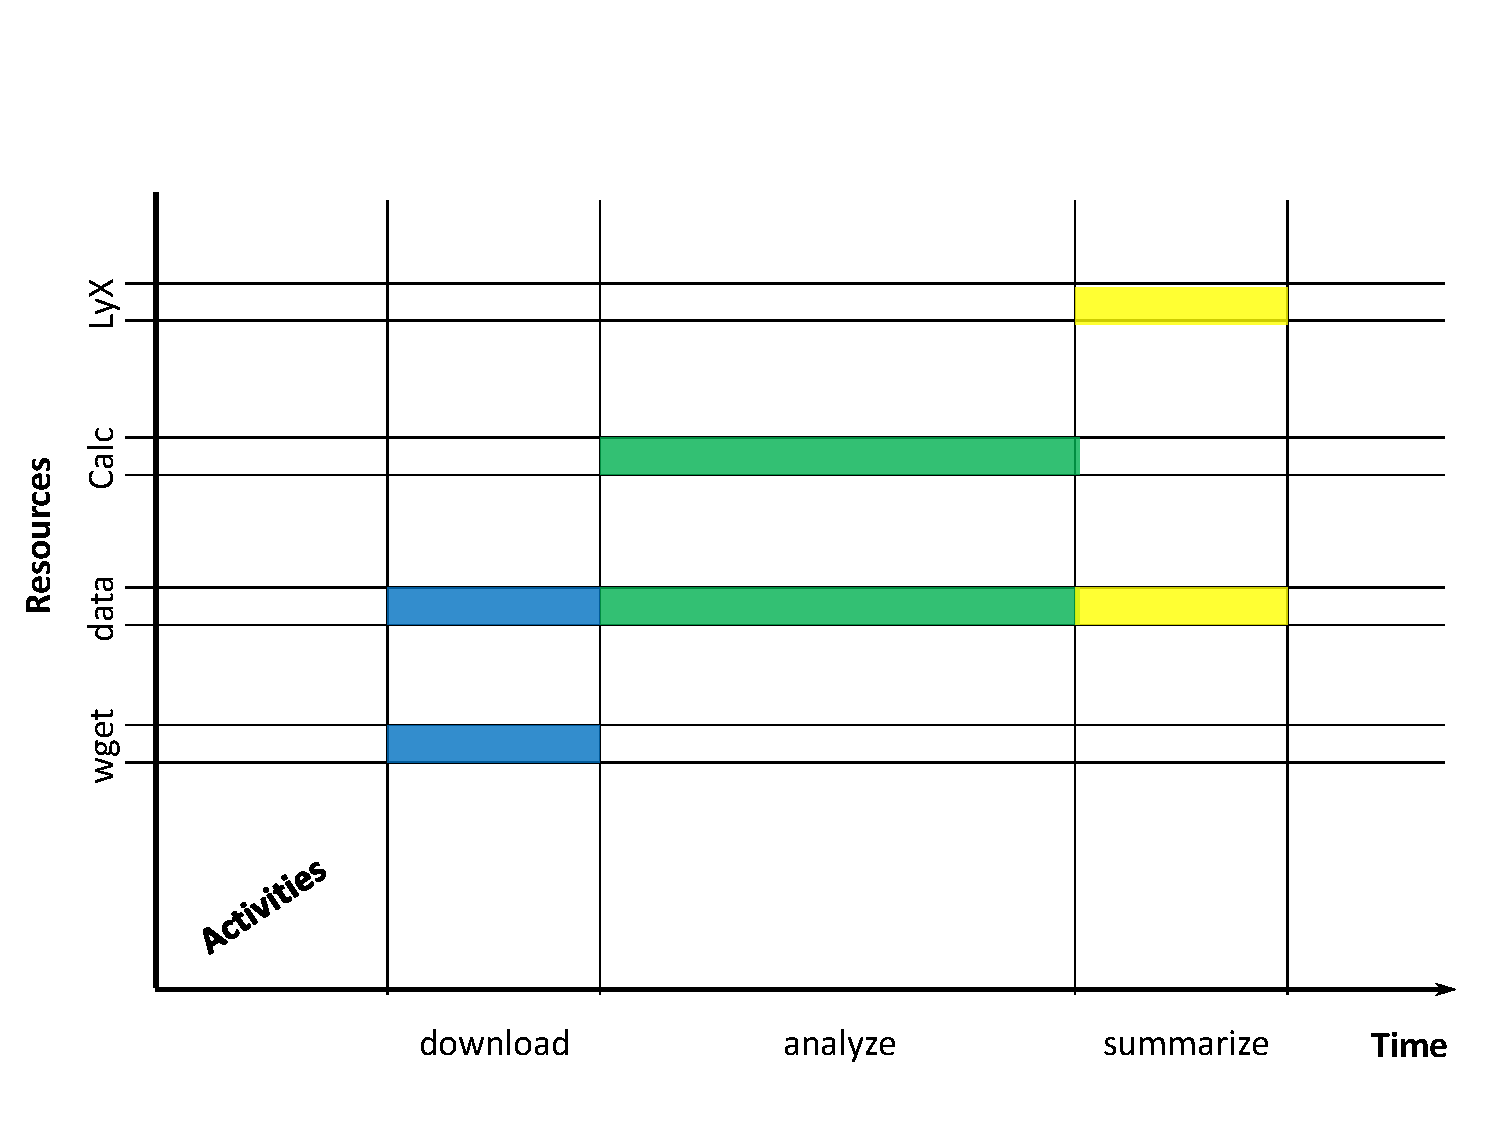
\includegraphics[scale=0.5]{prov-pieces}
\caption[Provenance for the creation of a table]{How provenance scatters throughout a table creation process. \texttt{wget} is used as an example of data download tools, \texttt{Calc} as an example of data analysis tools, and \texttt{LyX} as an example of table making tools.}
\label{prov-pieces}
\end{figure}
All these pieces of information can be captured by the authors if they are informed of the list of 
information items they need to record and they pay sufficient attention at certain time points where 
certain information pieces are available, but to capture them, the authors would spend time learning the list of necessary provenance items, and would quite often get 
distracted from their writing and table creation work. Given that doing research based on data is 
resource intensive and requires concentration, capturing provenance during writing brings no 
immediate benefit but lowers the productivity of the authors, so authors do not have incentives to 
record provenance unless they are required to do so. Even if they really would like to record all the 
details of the computational experiments they are carrying out, they are highly likely to miss some 
pieces of provenance that are not so obvious to and cannot be remembered later by human beings. 
%The benefit of having provenance information captured and properly stored comes later when some readers of the publication would like to better understand, validate and/or reproduce the published results, usually with an intention to use the result producing software for further research.

%So we see that provenance of research publication preparation shows its importance some time after 
%the publications have been created, although its importance has already been widely recognized by 
%readers and the future selves of authors. The problem is that provenance gets lost, piece by piece, 
%after the creation of publications, at a rate depending on how well the authors keep or memorize the 
%details of the publication preparation process.

\section{Possibility of developing tools to alleviate the situation}
\label{sec:possibility}
We argue that it is possible to develop tools to alleviate the situation that important provenance gets lost due to lack of awareness or timely capturing. These tools should have the following features.
\begin{itemize}
\item \emph{Knowledge of provenance.} i.e., they have the knowledge of provenance that is necessary to capture.
\item \emph{Automatic capturing mechanism.} i.e., they support a provenance capturing mechanism that requires very little explicit input from the authors.
\item \emph{Sufficient functionality.} i.e., they support a wide range of functions authors need to perform computational experiments and to prepare research publications.
\end{itemize}
We discuss the possibility of these tools based on the features they should have.

Knowledge of provenance could be encoded and stored in these tools, e.g., in the form of an ontology. 
Existing workflow systems that enable replications of computational experiments already have the 
necessary knowledge of provenance, which our tools could inherit.

The automatic capturing mechanism is possible to implement because information about data, their stewardship 
activities, and agents is all available, or could be adapted to become available to certain software 
agents, since most of the operations of the computational experiments the authors perform are carried 
out with software. (Exceptions include data being noted down or copied with a pen on a piece of paper, 
but even in this case, if the authors adapt to the use of software tools and input/copy data with such 
tools on the hard drive, the automatic capturing mechanism would apply.)

To be specific, we go over the 
listed provenance items in the running example mentioned above. 
\begin{itemize}
\item Information about the original data such as its download URL is known by the download software, 
because the software needs the URL to download the data. 
\item So is the starting and ending times of the downloading activity. 
\item The user account system knows who downloads the data. 
\item The API documentation of the data analysis software package is available as part of the software 
package. 
\item Information about software parameter values and function calls is known to the software agents who 
configure the software and invoke these functions. In the case where the users need to edit a 
configuration file to change software parameter values, a software agent that can do these edits with 
function invocations could be introduced, which knows the parameter values used for each function call.
\item The person, the software and the times related to the table making activity are known by the user 
account system and the table making software itself.
\end{itemize}
%We argue that only physical, syntactical and semantic changes of data are activities worth our attention. Data representation efforts such as making the summary table have nothing to do with replicating the final results, which is a special kind of data, thus creating the representations of results does not need to be included in the provenance of the results.

Sufficient functionality is guaranteed because provenance aware versions of the existing software based on proper domain ontologies that performs data stewardship activities can be developed. Such software has all the functions current authors need to produce research publications. (They are just using the provenance unaware existing software to prepare research publications now.) 

To wrap up, our provenance capturing tools are provenance aware versions of existing tools used by authors of research publications. These tools get the knowledge of necessary provenance needed from the domain ontologies, and capture provenance as the authors are using the software to prepare publications -- no need to ask the authors to explicitly note down anything they have done because all they have done are already captured at the time of doing.

\section{Contributions of the work in this thesis}
\label{sec:contribution}
The goal of the thesis is to design a paradigm of preparing research publications to overcome the problems associated with provenance capturing, namely lack of awareness of necessary provenance items and lack of incentive to capture provenance in a timely manner. The paradigm is to create publications with libraries that transparently capture the proper provenance information on a portable platform.

The proper provenance information to be captured is defined in an ontology designed to model the preparing process of research publications. Although there are general ontologies for provenance\footnote{PROV-O: The PROV Ontology. Available at http://www.w3.org/TR/prov-o/} and for publications and citations\footnote{Introduction to SPAR. Available at http://sempublishing.sourceforge.net/}, ontologies describing the process of publication preparation do not exist yet. The hypothesis to justify for this contribution is that the developed ontology is more useful than existing ontologies in the use case of modeling research publication preparation process.
%Unlike models for computational experiments, the ontology presented in this thesis pays special attention to the human factor in the process, which is a significant feature of the publication preparing process compared with the computational experiment workflows. The provenance capturing mechanism is driven by the ontology.
%capturing architectures and recording protocols developed for capturing provenance in computational experiments \cite{groth2006architecture, groth2009recording}\comment{find difference in our mechanism}, and ontologies for semantic

Transparent provenance capturing means the authors do not need to explicitly input provenance in order to record it, and they are allowed to work in their familiar computational environments. The capturing actions happen without interrupting the authors' ongoing work. The hypothesis to justify for this part of the work is that the specified mechanism is more useful than existing mechanisms such as creating workflows in capturing provenance for research publications.

A portable platform is a software package or a Web application that runs on some environment that is available on all the popular computational systems, such as a Java program which runs on the Java Virtual Machine, a Python program which runs with the Python interpreter, or a Web based application written in HTML, JavaScript and/or PHP scripts which runs on any of the mainstream Web browsers. Preparing research publications based entirely on a portable platform eliminates the necessity of capturing provenance down to the computer system level. Two desirable features for the platform are that 1) it should supply all the functions needed in creating research publications, and 2) these functions can be used in a way that is similar to the software packages the author is used to working with. To ensure the first feature, the platform needs to be extensible, better if it already has a strong development community to supply a plethora of evolving modules. The second feature requires that the platform supports popular interactive editing modes widely accepted in the research community. Examples include those seen in research software packages such as MATLAB and R. The hypothesis to justify for this part is that the implemented platform fulfills the requirements placed by the transparent provenance mechanism, so it really is a proof-of-concept prototype. 

To sum up, contributions of the work in this thesis are:
\begin{itemize}
\item the creation of an ontology for capturing provenance in the process of research publication preparation, along with an objective evaluation;
\item the specification of a provenance capturing framework driven by the ontology. The framework makes the provenance capturing actions transparent to the authors of research publications; and 
\item the implementation of a provenance aware publication preparing platform prototype that reflects most of the desired features for the specified provenance capturing mechanism.
\end{itemize}

%At the time of proposal, the focus will be on the design of the provenance capturing ontology and the evaluation method of it.

The remainder of this thesis is organized as follows. Chapter~\ref{related-work} discusses related work.
Chapter~\ref{research-approach} presents the research approach in detail. 
Chapter~\ref{ch:ontologies} lists the PROV-PUB-O ontology files.
Chapter ~\ref{ch:case-study} presents the details of the case study the thesis work is based on,
%Survey results justifying the effectiveness of the approach are given in Chapter \ref{survey-results}. 
%. Further discussions about this work and conclusions are given in Chapter \ref{discussions-and-conclusions}
and future work is discussed in Chapter~\ref{future-work}.

%%% Local Variables: 
%%% mode: latex
%%% TeX-master: t
%%% End: 
 % introduction
\chapter{RESEARCH APPROACH}
\label{research-approach}

% three requirements of the proposed authoring paradigm


\section{PROV-PUB-O: a provenance ontology for research publications}
This section presents the approach to the creation of an ontology for capturing provenance in the process of preparing research publications. The ontology is divided into two parts. 

The first part --- Section~\ref{subsec:structure} --- describes the structure of a research publication. We base our work on the Document Components Ontology (DoCO), which is one of the Semantic Publishing and Referencing Ontologies (SPAR). SPAR focuses a lot on modeling citations and bibliographic references. Four out of the eight ontologies in SPAR deal with citations and bibliographic references. (They are CiTO, the Citation Typing Ontology, FaBiO, the FRBR-aligned Bibliographic Ontology, BiRO, the Bibliographic Reference Ontology, and C4O, the Citation Counting and Context Characterization Ontology.) So SPAR is good for modeling the linkage between publications. 

%why we need to model document structure
In this thesis we focus on the reproducibility of a certain publication, so we do not delve deep into citations and bibliographic references as they have nothing to do with the computational experiments presented in the current publication. We model the structure of a research publication because experimental results must reside somewhere in the publication. Textual elements in the publication provide contextual information and explanation for the reported results. Although these elements are not parts of the process leading to the reported results, they are documentation that help readers to correctly interpret the results, so we include structural elements of research publications in the provenance.

We do not want an ontology with as many classes, properties and constraints as in DoCO. The idea is to select the minimal set of ontology elements from DoCO and define subclasses and properties to get a small ontology just sufficient for the purpose of describing the reported result (such as figure and table) containing parts of the research publications in the context of document components. For example, we just want to describe Figure X resides in Section Y which is part of Chapter Z which is part of Document W, and we do not need the capability of checking whether Section Y is a valid section by constraints such as ``sections cannot be back matters or body matters or chapters or ...'' 

The second part --- Section~\ref{subsec:process} --- describes the process leading to the reported results. It is a specialization of the W3C Provenance Ontology (PROV-O) for the use case of research publication preparation. We base the development of PROV-PUB-O on PROV-O because using general provenance ontologies such as PROV-O proves to be an effective way to keep track of the lineage of the source data and the changing processes leading to the final results. 

The goal of the specialization is to make the specialized ontology, namely PROV-PUB-O, detailed enough to enable the creation of \emph{executable provenance graphs} (EPGs). In an EPG, the semantics of each element in the process leading to the reported results is well defined, so the replication of the process becomes straightforward. Moreover, the process described with an EPG can even be used to validate the scientific conclusions by allowing readers to adapt the experiment reported in the paper and carry out their own studies.

PROV-PUB-O is further divided into two smaller ontologies: PROV-PUB-O/S for the structural model and PROV-PUB-O/P for the process model. We divide PROV-PUB-O in this way because we find that PROV-PUB-O/S alone can be used by publishing agents to describe typical research publications. 

The hypothesis to justify for PROV-PUB-O is that it is more usable than PROV-O in modeling research publication preparation process in the domain of earth science for the purpose of replicating data transformation processes and validating scientific conclusions.

\subsection{PROV-PUB-O/S: publication structure modeling}
\label{subsec:structure}

The development of PROV-PUB-O/S follows the following principles:
\begin{itemize}
	\item Minimalism on classes --- meaning to make the number of constraints to its minimum and only define necessary classes to flatten the learning curve, quicken the prototyping and iterating processes.
	\item Rich on properties --- meaning to have multiple ways of expressing relations among classes, so that users are more likely to find a way that is easy to use for them. To avoid incomplete query results due to multiple ways of relation expression, users can choose to follow one particular way but they are not forced by being given only one way.
	\item Leave the decision for dependencies to the users --- meaning that we do not hard code dependencies to other ontologies which force the users to accept them. We just provide suggestions in documentation and let the users decide whether to accept the suggested dependencies.
\end{itemize}

% where do these principles come from?
These principles are based on intuitions. The first principle, minimalism on classes, is based on the intuition that too many classes confuse the user at the very first moment s/he looks at the ontology. It is even worse if some of these classes bear unfamiliar names to the user and constraints requiring certain expertise in OWL. The user needs to learn the inner logic among the vast number of classes to make sure s/he does not break any rule in the system. Too many classes with too many constraints also make the ontology hard to maintain. Every little change may break the consistency of the whole system. When designing PROV-PUB-O/S, we use only the most commonly accepted words such as chapters and sections for class names, and limit the number of constraints to the minimum. In fact, we do not introduce any intra-class constraints other than super/sub-class hierarchy.

The second principle, rich on properties, is based on the assumption that people have very different ways of saying the relations between class instances. For example, the part-whole relation between a figure B and a publication A may be represented as ``A contains a chapter (that contains a section) that contains B'' or ``A has a figure B''. Some people may prefer swapping the positions of A and B and saying ``B is in A'', so if we force the users to use only one way of saying a certain relation by providing in the ontology only one way of saying it, users are likely to find the ontology very cumbersome to use. This is very different from the situation of having a lot of classes, because each class usually represents a distinct type of things, but properties can provide alternative ways of achieving the same linking among classes. The more the number of classes, the more time it takes to find the right ones to use; the more alternative ways of linking classes, the less time it takes to find a proper way, and the more likely a preferable way is found. In PROV-PUB-O/S, shortcut properties are introduced to allow users to represent for example a figure is in a publication directly, instead of forcing the users to express the same meaning with a figure-section-chapter-publication chain of part-whole relations. 

The third principle, leaving the decision for dependencies to the users, is a natural corollary of the first principle, because subclassing or equivalent-classing means to force the user who wants to use a certain class in the ontology in question to use another class from another ontology, since instances of the class wanted automatically become also instances of the other class in the other ontology. It is virtually adding more classes, and maybe more constraints along with these classes to the ontology in question. Making small ontologies depend on a much larger ontology exposes the users to the complicated class system of the latter and steepens the learning curve of the small ontology dramatically. In PROV-PUB-O/S, subclassing assertions are only suggested in comments and not included in the ontology source file but put in separate bridging ontologies for the users familiar with the depending ontologies to choose to use.

% how these principles are followed
Rather than starting from scratch, we refer to existing models for document structures to get the common vocabulary to follow. Document structure models such as the Document Components Ontology (DoCO)\footnote{DoCO, the Document Components Ontology: \url{http://purl.org/spar/doco}, accessed on October 10th, 2015} are usually based on structural patterns \cite{di2014dealing} and rhetorical structure theory (RST) \cite{taboada2006rhetorical}.

Here we take DoCO as an example. DoCO defines structural (e.g. block, inline, paragraph, section, chapter, and so on --- meaning what the component looks like) as well as rhetorical (e.g. introduction, discussion, acknowledgements, reference list, figure, appendix, and so on --- meaning what role the component plays in the document) document components.

Figure~\ref{fig:doco} shows the components of DoCO and the respective classes included in these components.
\begin{figure}
	\centering
	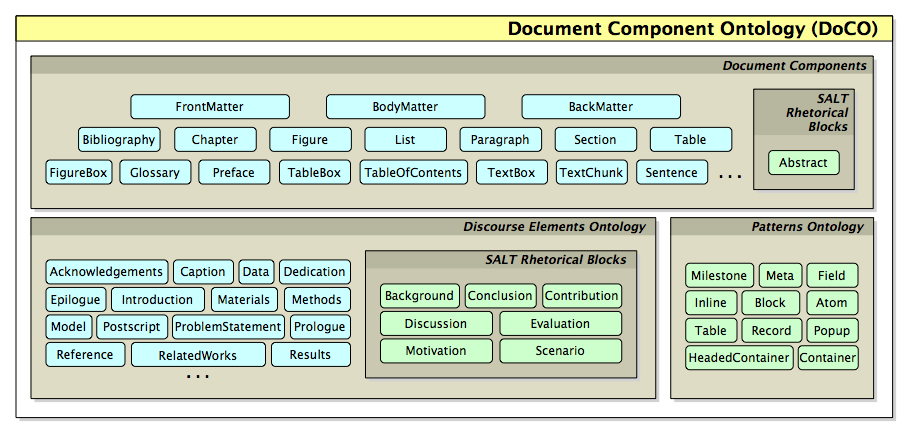
\includegraphics[width=\textwidth]{doco-architecture.png}
	\caption[Architecture of DoCO]{Architecture of DoCO, the Document Components Ontology}
	\label{fig:doco}
\end{figure}

Structural document component types are closely related to the typesetting of the component contents. For example, if a block of text consisting of a title and several paragraphs is known to be a chapter, then at the time of rendering this block, the title can be made larger, proper font and size can be set for the content paragraphs, and the proper spacing can be set between this block and the blocks previous and next to it. Therefore, each structural document component type is like a class used to label HTML elements, and to be rendered according to class styles defined in Cascading Style Sheets (CSS).

Rhetorical document component types are completely irrelevant to typesetting --- just knowing a block of text is an ``introduction'' has nothing to do with properly formatting it. Rather, rhetorical types focus on the \emph{relations} between document parts, so these types are actually \emph{types of relations}. For example, the ``introduction'' component of a paper is usually a chapter, but theoretically it can be a section or even just a paragraph, leading to very different typesetting options. But just look at how we call this ``introduction'' component -- we call it ``introduction \emph{of} a paper'', i.e., an introduction block is always \emph{of something}. It does not make sense to have a ``floating'' introduction attached to nothing. 

In light of this relational perspective of rhetorical types, we make the following changes from DoCO:

\begin{itemize}
	\item The deo:Introduction (\url{<http://purl.org/spar/deo/Introduction>}) class is changed to the pub:introduction property. The prefix deo expands to http://purl.org/spar/deo/ and stands for The Discourse Elements Ontology\footnote{The documentation of the Discourse Elements Ontology is available at http://www.essepuntato.it/lode/owlapi/http://purl.org/spar/deo/, accessed on October 6th, 2015.}, and the prefix pub is for PROV-PUB-O\footnote{PROV-PUB-O is not officially published yet. It is temporarily hosted at \url{http://orion.tw.rpi.edu/~fulinyun/ontology/prov-pub/}, accessed on October 10th, 2015.}. The class pub:Block is the union of pub:Chapter and pub:Section.
	\item The classes sro:Abstract (\url{<http://salt.semanticauthoring.org/ontologies/sro#Abstract>}), deo:Background, deo:Conclusion, deo:Contribution, deo:Discussion, deo:Evaluation, deo:Motivation, deo:Scenario, doco:RelatedWork, \url{doco:Acknowledgements}, doco:Appendix and doco:Foreword are changed in the same manner as deo:Introduction. The prefix sro expands to  http://salt.semanticauthoring.org/ontologies/sro\# and stands for SALT (Semantically Annotated \LaTeX \cite{groza2007salt}) Rhetorical Ontology\footnote{According to http://lov.okfn.org/dataset/lov/vocabs/sro, accessed on October 9th, 2015, this ontology is still offline. Its namespace domain semanticauthoring.org changed owner and the ontology file is missing.}.
	\item The deo:Caption (\url{<http://purl.org/spar/deo/Caption>}) class is changed to the pub:caption property, whose range is xsd:string (\url{<http://www.w3.org/2001/XMLSchema#string>}).  the namespace xsd expands to \url{http://www.w3.org/2001/XMLSchema#} and stands for W3C XML Schema Definition Language\footnote{The documentation of the W3C XML Schema Definition Language (XSD) is listed at \url{http://www.w3.org/2001/XMLSchema#}, see the links in the ``Normative References'' section, accessed on October 6th, 2015.}.
%	\item The sro:Abstract ($<$http://salt.semanticauthoring.org/ontologies/sro\#Abstract$>$) class is changed to the pub:abstract property, whose domain is pub:Block, and range is pub:Document. The prefix sro expands to \comment{get rid of abstract since it's not relevant to tables and figures.} http://salt.semanticauthoring.org/ontologies/sro\# and stands for SALT (Semantically Annotated \LaTeX \cite{groza2007salt}) Rhetorical Ontology. The prefix doco expands to http://purl.org/spar/doco/, and the prefix dcterms expands to http://purl.org/dc/terms/, meaning DCMI (Dublin Core$^{\textregistered}$ Metadata Initiative) Metadata Terms\footnote{DCMI Metadata Terms: http://dublincore.org/documents/dcmi-terms/}.
%	\item The sro:Background class is changed to the pub:background property, whose domain is (doco:Chapter or doco:Section) and (dcterms:isPartOf some doco:BodyMatter), and range is pub:Document. 
%	\item Classes sro:Conclusion, sro:Contribution, sro:Discussion, sro:Evaluation, sro:Motivation, sro:Scenario are changed in the same manner as sro:Background. Note that these classes are different from sro:Abstract in that they cannot be part of the front matter component of a document.
	%\item The class deo:Acknowledgements \comment{not sure yet.} The prefix deo here expands to http://purl.org/spar/deo/ and stands for the Discourse Elements Ontology\footnote{The Discourse Elements Ontology: http://purl.org/spar/deo}.
\end{itemize}

In addition to the changes above, PROV-PUB-O/S is much smaller than DoCO in its number of classes and free of complicated constraints that may confuse the users, yet expressive enough to describe typical research publications without missing any interesting parts. For example, 
\begin{itemize}
	\item In DoCO there are classes representing paragraphs and sentences, which we do not include in PROV-PUB-O/S because section level location is accurate enough for figures and tables. It is accurate enough to say ``Figure X is in Section Y''. It is probably an overkill to say ``Figure X is in the n-th paragraph of Section Y''. However, we did define a result container class and the users can extend PROV-PUB-O/S by defining subclasses of it to describe application specific result containers.
	\item DoCO also contains a ``figure box'' class to represent the physical space within a document that contains a figure and its caption. Such a fine-grained dissection of a figure is probably not necessary for research publications. It is usually clear enough to say ``Figure X has a caption saying Y'', so we define the pub:caption property to describe the relation between a figure and its caption.
	\item A doco:Section can only contain (represented by the pattern:contains property in DoCO: \url{<http://www.essepuntato.it/2008/12/pattern#contains>}) some doco:Paragraph or doco:Section instances, so if we want to express that ``a section contains a figure'' with DoCO, we must be knowledgeable enough to avoid using the pattern:contains property that comes with DoCO but to use a less strict property such as dcterms:hasPart (\url{<http://purl.org/dc/terms/hasPart>}). This is an example showing the confusion caused by complicated constraints. Obviously the constraint is defined without considering the need to locate a figure at the section level. In PROV-PUB-O/S, ``a section/chapter/publication has certain figures'' is expected to be asserted frequently, so the pub:hasFigure property is introduced to make this kind of assertions really easy to make. A reminder of not asserting pub:hasFigure to be a sub-property of pattern:contains is given in the rdfs:comment (\url{<http://www.w3.org/2000/01/rdf-schema#comment>}) annotation to stop users from committing the error. 
\end{itemize}
This follows the principles of minimalism on classes and rich on properties.

The resulting PROV-PUB-O/S ontology\footnote{PROV-PUB-O/S is not officially published and is temporarily hosted at \url{http://orion.tw.rpi.edu/~fulinyun/ontology/prov-pub/prov-pub-s.ttl}, accessed on October 10th, 2015.} follows a minimalist approach on class definitions to be a small ontology just sufficient for the purpose of describing the results and the parts of the research publications that contain them. Figure~\ref{fig:prov-pub-s-classes} and Figure~\ref{fig:prov-pub-s-properties} shows the classes and properties in PROV-PUB-O/S, respectively.

\begin{figure}
	\centering
	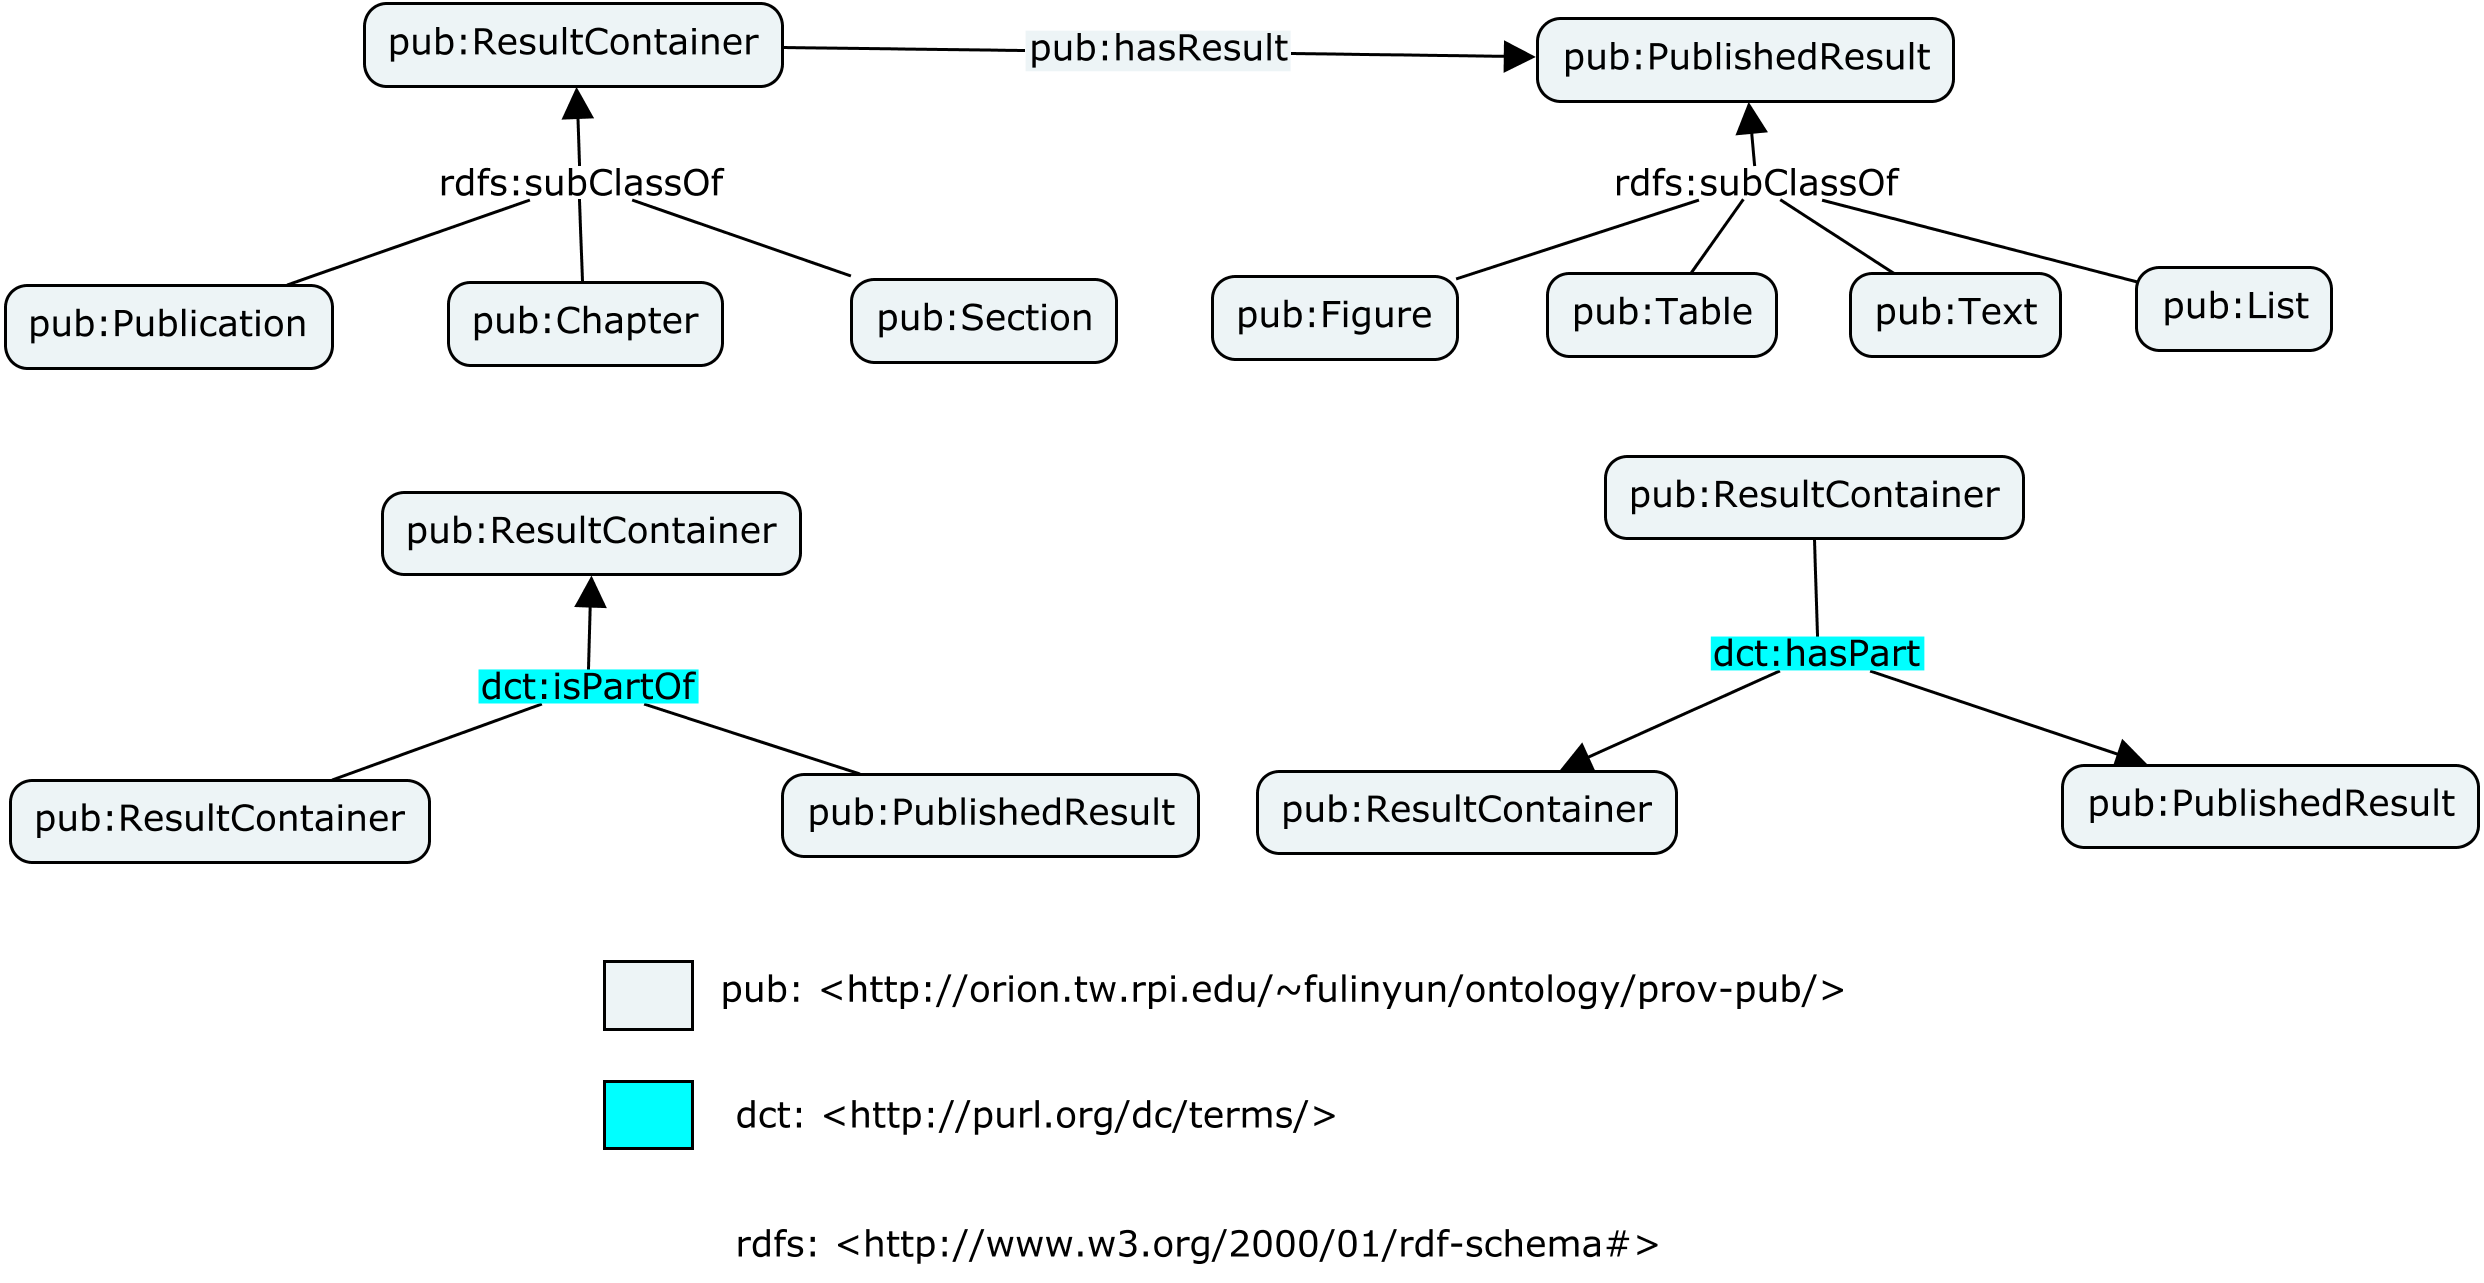
\includegraphics[width=\textwidth]{model/ontology/prov-pub/prov-pub-s-classes.png}
	\caption{Classes in PROV-PUB-O/S}
	\label{fig:prov-pub-s-classes}
\end{figure}

\begin{figure}
	\centering
	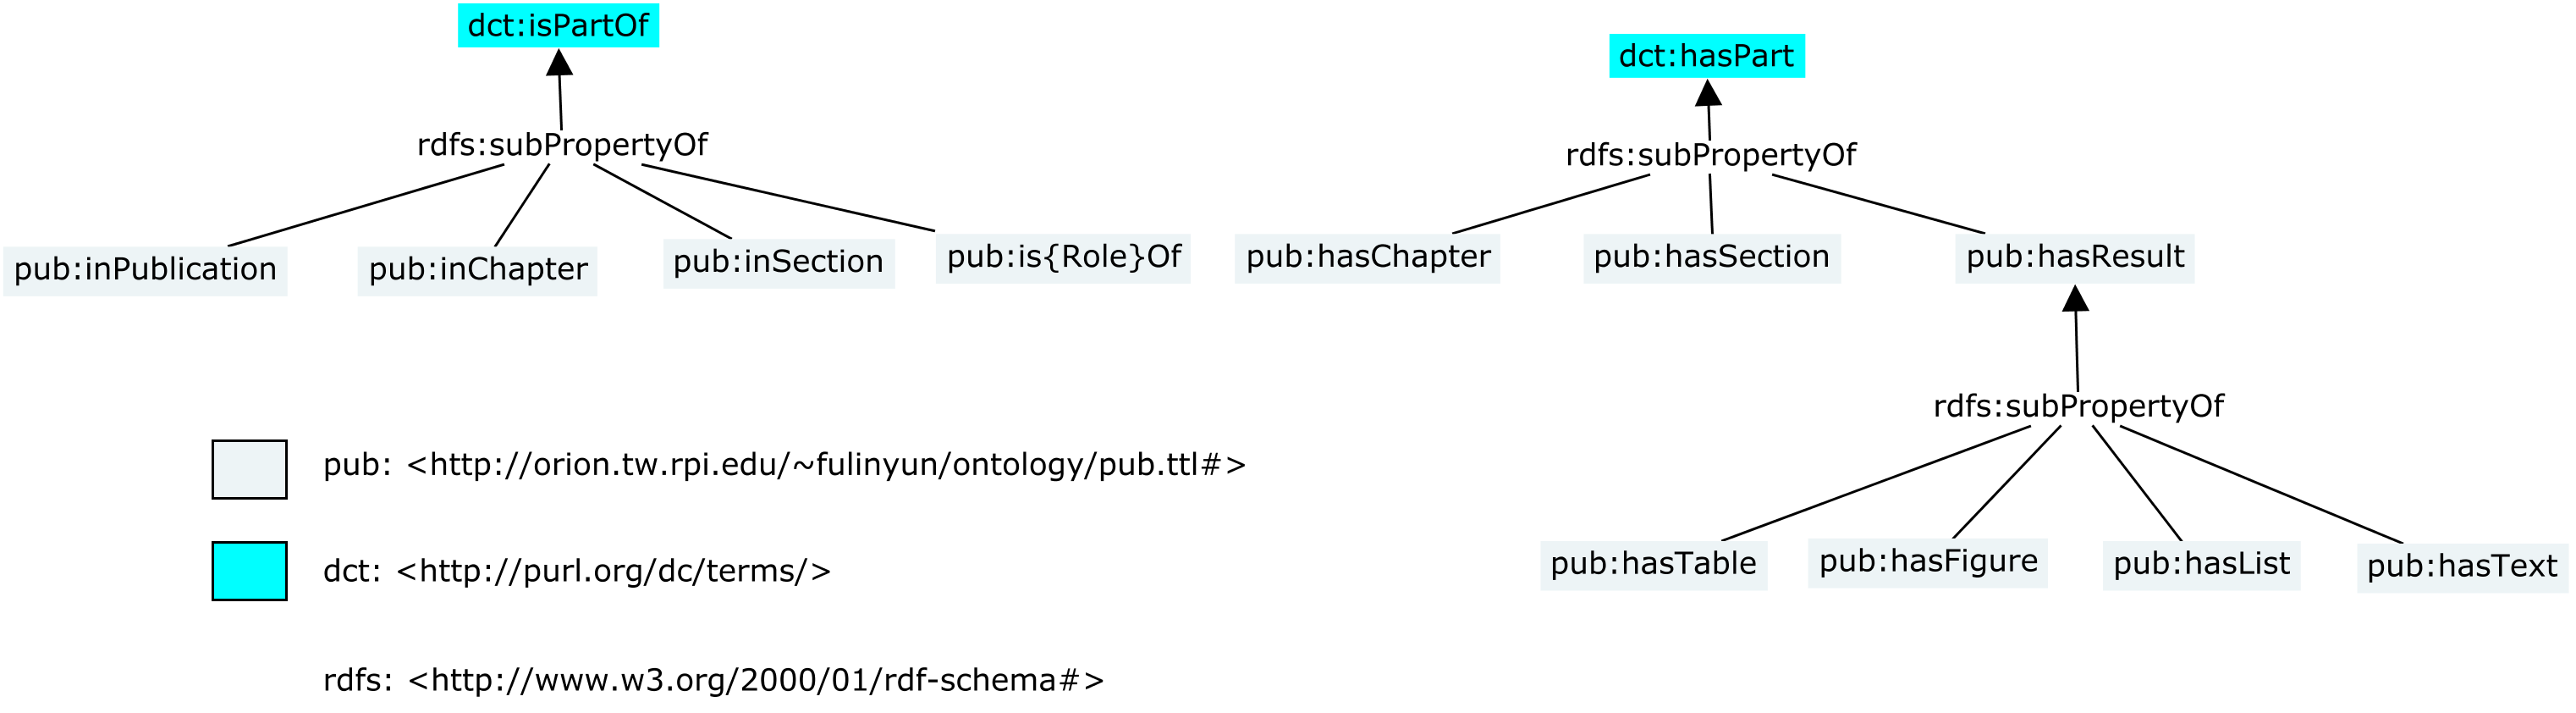
\includegraphics[width=\textwidth]{model/ontology/prov-pub/prov-pub-s-properties.png}
	\caption[Properties in PROV-PUB-O/S]{Properties in PROV-PUB-O/S, where pub:is{Role}Of represents the role indicating properties such as pub:isIntroductionOf, pub:isAbstractOf, and so on}
	\label{fig:prov-pub-s-properties}
\end{figure}


An important conceptual deviation of PROV-PUB-O/S from DoCO is that in DoCO, tables and figures are considered blocks of documents the same way as chapters and sections, but in PROV-PUB-O/S, they are considered research results instead of normal document parts. Other block elements such as chapters and sections are also considered result containers in PROV-PUB-O/S. They are defined to serve the function of locating interesting results in research publications. We stop our document part modeling at the section level because sections are the most fine-grained elements that have (numerical) labels such as ``Section 2.1.1'' and/or captions such as ``PROV-PUB-O/S: publication structure modeling''. This is not the case for paragraphs and sentences. Note that subsections of a section is also instances of pub:Section. 
%Minimalism here means to only define a set of ontology elements that must be defined together to ensure their proper function, so PROV-PUB-O/S does not 
%assert any of its classes to be a subclass or equivalent class of a class from another ontology if that assertion is not necessary for PROV-PUB-O/S to 
%function properly.

Four types of published results are defined in PROV-PUB-O/S: tables, figures, lists and textually described results. 

PROV-PUB-O/S can also be used together with the BibTeX ontology\footnote{The BibTeX ontology: \url{<http://purl.org/net/nknouf/ns/bibtex>}, accessed on October 10th, 2015.} or the Bibliographic Ontology\footnote{The Bibliographic Ontology: \url{<http://purl.org/ontology/bibo/>}, accessed on October 10th, 2015.}. Since no subclassing link to the related ontologies is hard coded in PROV-PUB-O/S, the users have the choice of whether 
to link PROV-PUB-O/S with these three ontologies (and thus depend on them) and to what extent. 

Two typical ways of linking PROV-PUB-O/S with its related ontologies are subclassing and double-classing. Subclassing means to assert that a class in PROV-PUB-O/S is a subclass of 
a class in one of the related ontologies. For example, the user could optionally assert that pubs:Chapter is a subclass of 
doco:Chapter to make every instance of pubs:Chapter automatically also an instance of doco:Chapter. Double-classing means to assert that an instance of 
a PROV-PUB-O/S class is also an instance of another class in a related ontology. For example, an instance can be asserted as both a pubs:Publication 
and a bibo:Document.

Following the principle of Leaving the decision for dependencies to the users, subclassing and double-classing suggestions are given for each class in PROV-PUB-O/S 
in case the user of the ontology 
wants to reuse the classes and constraints defined in the related ontologies.

Three bridging 
ontologies\footnote{Like PROV-PUB-O itself, these bridging ontologies are not officially published yet, and are temporarily hosted at \url{http://orion.tw.rpi.edu/~fulinyun/ontology/prov-pub/prov-pub-s-doco.ttl}, \url{http://orion.tw.rpi.edu/~fulinyun/ontology/prov-pub/prov-pub-s-bibtex.ttl} and 
\url{http://orion.tw.rpi.edu/~fulinyun/ontology/prov-pub/prov-pub-s-bibo.ttl}, accessed on October 10th, 2015.} are provided in case a user wants to accept all the suggested subclassing links from
PROV-PUB-O/S to one of its related ontologies. Each bridging ontology is exclusively composed of assertions of the form ``pubs:X rdfs:subClassOf doco:Y'' 
such as ``pubs:Chapter rdfs:subClassOf doco:Chapter''. Double-classing suggestions cannot be encoded in the form of bridging ontologies because they do 
not require any assertion at the schema level.

There are existing ontologies, such as the GCIS ontology \cite{ma2014ontology}, that also have classes to represent document components such as chapters, but we prefer not reusing from such application ontologies because PROV-PUB-O/S is considered to be a general ontology for all kinds of research publications, and it is logical to have application ontologies make subclassing and/or equivalent-classing assertions to general or domain ontologies, but not the other way around.
%The general hypothesis to justify here is that PROV-PUB-O/S are more usable than DoCO for the task of describing the structure of a research publication, and a specific hypothesis is that properties in PROV-PUB-O/S are more usable than their corresponding rhetorical concepts in DoCO for describing publication components. We conducted user survey to collect opinions about pairs of RDF statement groups such as
%\begin{quote}
%	\begin{tabular}{l}
%	abs a Section;\\
%	 \hspace{1em}isAbstractOf article.\\
%	 \hspace{3em}vs.\\
%	abs a Abstract;\\ 
%	 \hspace{1em}isPartOf article.
%	\end{tabular}
%\end{quote}
%, that is, whether it is better to describe the relation between an article and its abstract component by saying that ``that section is the abstract of the article'' or that ``that section is an abstract, and it is part of the article''. Here we omit all the RDF prefixes in the statements emphasize the modeling rationale.

\subsubsection{Lessons learnt}
The three principles of designing a usable ontology --- minimalism on classes, rich on properties and leaving the decision for dependencies to the users --- is developed as we had finished the conceptual modeling and started writing the ontology in Turtle format, which was considered just a ``finishing up'' work. Documentation requires numerous decisions to make about wordings, definitions or even formatting. The workload increases quickly with the number of classes and dependencies in the form of subclassing or equivalent-classing. One change may trigger a whole lot of change all over the ontology to keep it consistent.

Online and standalone tools are helpful in decreasing the amount of manual work in creating and formatting ontology files and creating documentation. EasyRdf\footnote{EasyRdf converter: http://www.easyrdf.org/converter, accessed on October 10th, 2015.} was used to convert ontologies in RDF/XML format to Turtle format. rdfEditor\footnote{rdfEditor: https://bitbucket.org/dotnetrdf/dotnetrdf/wiki/UserGuide/Tools/rdfEditor, accessed on October 10th, 2015.} was used to edit and validate the ontology files. Make sure to end each namespace properly with a slash (`/') or hash (`\#') character, since editors do not check for errors of this kind, and namespaces not properly ended would yield incorrect IRIs such as \url{<http://purl.org/ontology/biboDocument>} instead of \url{<http://purl.org/ontology/bibo/Document>}. LODE\footnote{Live OWL Documentation Environment: http://www.essepuntato.it/lode, accessed on October 10th, 2015.} was used to generate the draft of documentation for the ontologies. HTML Formatter\footnote{Free HTML Formatter: http://www.freeformatter.com/html-formatter.html, accessed on October 10th, 2015.} was used to format the draft documentation generated by LODE, and Word Wrap\footnote{Free online word wrap: http://appincredible.com/online/word-wrap/, accessed on October 10th, 2015.} was used to format the ontology file for inclusion in the appendix of this thesis.


\subsection{PROV-PUB-O/P: Result generating process modeling}
\label{subsec:process}
Results in research publications often are quite separated from the underlying collection and analysis of data. The grand goal of keeping track of provenance is to enable the readers to understand the process the authors have gone through to produce the reported results from the collected data.

Provenance describes the lineage of the source data and the changing processes leading to the final results for readers to correctly interpret report content. Provenance also enables readers to evaluate the credibility of the reported results by digging into the software in use, operations that have been taken, source data and responsible agents.

Using general provenance ontologies such as PROV-O\footnote{PROV-O: The PROV Ontology: http://www.w3.org/TR/prov-o/, accessed on October 22nd, 2015.}, the new W3C standard adopted in 2013, proves to be an effective way to keep track of the lineage of the source data and the changing processes leading to the final results.

However, in a specific domain of interest, a lot more contextual and operational information that the readers really care about could be added to RDF graphs created with such general ontologies to include much more operationally meaningful elements for automated processing of the provenance graphs.

\subsubsection{Example of direct use of PROV-O to record provenance}
PROV-O\footnote{Lebo, T., Sahoo, S., \& McGuinness, D. (2013). PROV-O: The PROV Ontology. Accessible at: http://www.w3.org/TR/prov-o/, accessed on October 22nd, 2015.} is a great advance based on its predecessors such as Proof Markup Language (PML) \cite{da2006proof} and the Open Provenance Model (OPM) \cite{moreau2011open}, Table 2 in \cite{ma2014ontology} gives a comparison of classes and properties of these three ontologies, which is shown in Table~\ref{tab:comparison}. From the table we could see that PROV-O filled in the blanks that are not established in PML and OPM. More classes and properties in PROV-O do not cause the ontology to be more complicated to understand because all these ontological elements are well organized into a simple framework shown in Figure~\ref{fig:prov-o}.
\begin{table}
	\centering
\caption{Similar classes and properties in PROV-O, OPM and PML}
\label{tab:comparison}        % \label command must always comes AFTER the caption
\begin{tabular}{|p{0.07\textwidth}|p{0.31\textwidth}|p{0.31\textwidth}|p{0.31\textwidth}|}
	\hline  & PROV-O & OPM & PML \\ 
	\hline Class-es & prov:Entity & opmv:Artifact & pmlj:Nodeset \newline (+pmlp:Information) \\ 
	  & prov:Activity & opmv:Process & pmlj:InferenceStep \newline (+pmlp:InferenceRule) \\ 
	  & prov:Agent & opmv:Agent & pmlp:InferenceEngine \\ 
	  & prov:Role & opmo:Role & Not established \\ 
	\hline Prope-rties & prov:used & opmv:used & pmlj:hasAntecedentList \newline (+pmlj:NodeSetList) \\ 
	  & prov:wasGeneratedBy & opmv:wasGeneratedBy & pmlj:isConsequentOf \\ 
	  & prov:wasAssociatedWith & opmv:wasControlledBy & pmlp:hasInferenceEngine \\ 
	  & prov:wasAttributedTo & Not established & Not established \\ 
	  & prov:wasDerivedFrom & opmv:wasDerivedFrom & Not established \\ 
	  & prov:wasInformedBy & opmv:wasTriggeredBy & Not established \\ 
	  & prov:actedOnBehalfOf & Not established & Not established \\ 
	  & prov:startedAtTime & opmv:wasStartedAt & Not established \\ 
	  & prov:endedAtTime & opmv:wasEndedAt & Not established \\ 
	\hline 
\end{tabular}
\end{table}
\begin{figure}
	\centering
	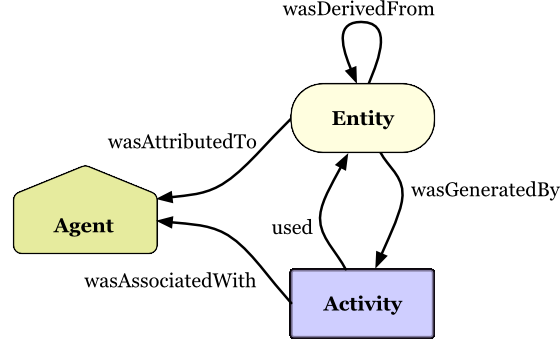
\includegraphics[width=0.7\textwidth]{prov-o.png}
	\caption{PROV-O framework}
	\label{fig:prov-o}
\end{figure}
For example, Figure~\ref{fig:gcis} shows what a typical provenance graph fragment looks like if it is created by reusing PROV-O.
\begin{figure}
	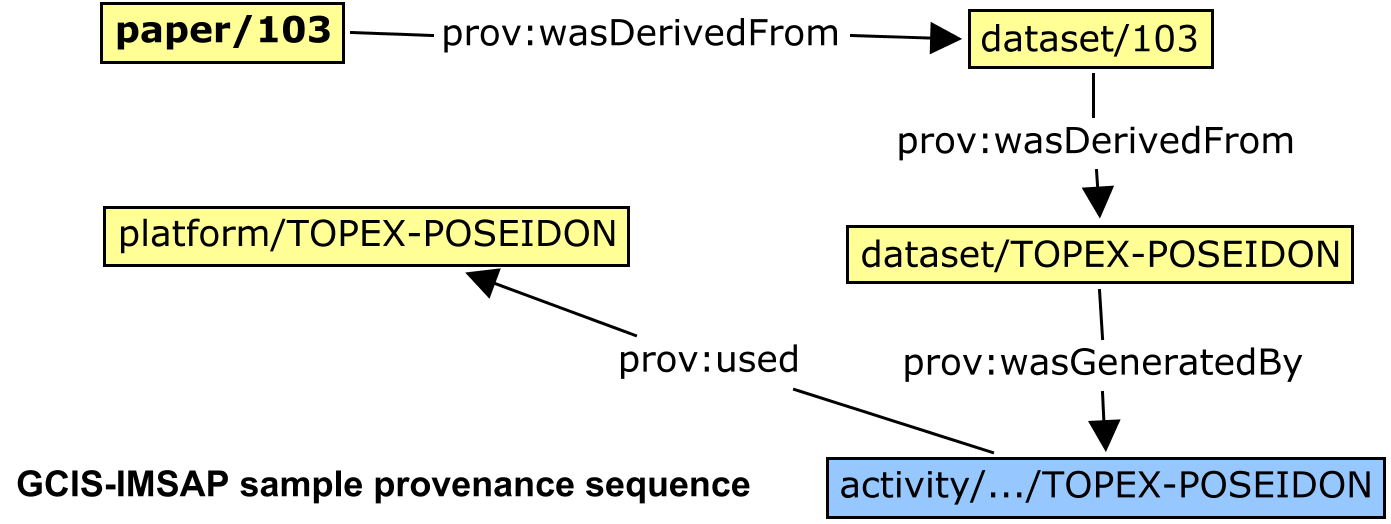
\includegraphics[width=\textwidth]{gcis-prov.png}
	\caption{Provenance graph fragment encoded in PROV-O}
	%\comment{to delete the caption inside the figure}
	\label{fig:gcis}
\end{figure}
The example is drawn from the Global Change Information System: Information Model and Semantic Application Prototypes (GCIS-IMSAP) project\footnote{Global Change Information System: Information Model and Semantic Application Prototypes: http://tw.rpi.edu/web/project/gcis-imsap, accessed on October 22nd, 2015.}. The project models and captures provenance information for the recent National Climate Assessment (NCA) draft report\footnote{The full draft for public review is available at http://downloads.globalchange.gov/nca/nca3-drafts/NCAJan11-2013-publicreviewdraft-fulldraft.pdf, accessed on October 22nd, 2015.} of the US Global Change Research Program (USGCRP).

From the provenance graph, we could get the information that the paper ``paper/103'' was derived from the dataset ``dataset/103'', which in turn was derived from the dataset ``dataset/TOPEX-POSEIDON'', which was generated by the activity ``activity/.../TOPEX-POSEIDON'' that used the platform ``platform/TOPEX-POSEIDON''. Irrelevant URI parts are omitted in the graph to make the meaning of the graph clear. Also note that all PROV-O properties use past tense verbs to emphasize that everything recorded in the provenance graph must be something that already happened.

Such information is quite useful for the general public to know the process of generating the reported results in the paper. However, for domain scientists who would like to verify the reported results or to base their new research on the work reported in this paper, the provenance graph is short on critical details such as:
\begin{itemize}
	\item How the reported results in ``paper/103'' were derived from ``dataset/103'', e.g., what data items were used to create a certain plot in the paper.
	\item How ``dataset/103'' was derived from ``dataset/TOPEX-POSEIDON'', e.g., what changes were made on what part of the original dataset to generate the derived one.
	\item How ``activity/.../TOPEX-POSEIDON'' used ``platform/TOPEX-POSEIDON'' to generate ``dataset/TOPEX-POSEIDON'', e.g., whether an algorithm and/or a model was used to deal with the raw data from the platform, what parameter values were used to run the algorithm and/or model.
\end{itemize} 
We define our provenance ontology for research publications, called PROV-PUB-O/P, by specializing the ``activity'' class and the ``used'' property in PROV-O to make the ontology suitable for capturing executable provenance in research publications.

Note that ``wasDerivedFrom'' do not need to be specialized because ``e1 wasDerivedFrom e2'' is a shortcut for ``a1 used e1; a1 generated e2'', where e1, e2 are PROV-O entities and a1 is an PROV-O activity. Neither do ``wasGeneratedBy'' since how an activity used its input entities already contains all the information needed for replicating the generation. The property ``wasGeneratedBy'' merely points out the output entity of the activity.

Interesting activities in the process of preparing research papers are all the changes of data, which can be classified into the following three categories:
\begin{itemize}
	\item Physical changes such as data download, copying, or sharing.
	\item Syntactical changes such as XML to JSON conversion.
	\item Semantical changes such as data analysis and transformation.
\end{itemize}
Each of the above changes corresponds to a certain way of data usage.

To capture these changes of data, four classes are defined in PROV-PUB-O/P: pub:DataChange for the general changes of data, pub:PhysicalChange for physical changes that keep data ``as is'' and only change the locations and access permissions of data, pub:SyntacticalChange for syntactical changes that keep the logical content of data intact and only change the formats and encodings of data, and pub:SemanticalChange for semantical changes that change the actual logical content of data. For most of the changes of data, it is the semantical changes that are of interest. If all these changes are marked and later queried, it would provide quite useful information of the published result generation process. However, physical changes and syntactical changes can also be critical for certain use cases. The case study we conducted on the 5 figures and 3 tables in Chapter 4 of NCA 2014 report showed that where the authors downloaded their source data and in what way the data were serialized play important roles in fully capturing the provenance of these figures and tables. In the cases where data analysis and transformation are straightforward or standardized, natural language descriptions of semantical changes could take the place of fully fledged source code containing pub:SemanticalChange activities, but the descriptions of the download and syntactical manipulation steps are easily overlooked and often insufficient for reproducing the published results. 

To further define specialized activities under and beyond the above three categories, we performed a case study on the 5 figures and 3 tables in Chapter 4 of the National Climate Assessment Report published in 2014 (NCA 2014). 

\subsubsection{Case study on the figures and tables in Chapter 4 of NCA 2014}
After a careful scrutiny of the 5 figures and 3 tables in Chapter 4 of NCA 2014, the following two types of recurring result generation paradigms are summarized:
\begin{itemize}
	\item Direct reuse of an existing result such as a figure. For example, Figure~4.1 in NCA 2014, ``Paths of Hurricanes Katrina and Rita Relative to Oil and Gas Production Facilities'', is just a slight adaptation of Figure~3 in the ``Natural Gas: Factors Affecting Prices and Potential Impacts on Consumers (GAO-06-420T)'' report. We argue that if both reports have their results recorded in provenance graphs with PROV-PUB-O/S, a much precise citation of the Figure~3 of the latter report could be provided in the previous report. We capture this kind of result generation process with the pub:Reuse class, which is a subclass of the prov:Activity class. This class is not a subclass of the ``change of data'' class pub:DataChange, because it does not actually happen on data, but on results.
	\item Step-by-step process including the initial download and possibly syntactical manipulation, the intermediate slicing, transformation and/or analysis, and the final plotting and/or summarization. For example, Figure~4.2 in NCA 2014, ``Increase in Cooling Demand and Decrease in Heating Demand'', is generated by downloading source data from a landing page on the NOAA National Climate Data Center Website by filling out a data request form, and then following the processing method described in the caption of the figure, followed by a plotting step not described at all.
\end{itemize}
Interesting findings from this case study include:
\begin{itemize}
	\item Physical changes of data can be quite complicated and yet easily overlooked. For example, to obtain a copy of the data used to generate Figure~4.2, the interested reader needs to somehow find the link to another page containing a data request form the landing page of the data source provided by the authors. For Figure~4.4, ``Projected Changes in Seasonal Precipitation'', downloading the source data requires the reader to register at the Website and wait for the approval of the administrator of the Website, which took me 4 days. The information about how to fill out data request forms and about the registration process is missing in the provenance graph for NCA 2014.
	\item Syntactical changes of data can be avoided by properly using the function of format selection provided by the data portals. For example, the data request form at \url{http://www7.ncdc.noaa.gov/CDO/CDODivisionalSelect.jsp#} for the data source of Figure~4.2 has an option group to let the users select the format of the requested data file, and space separated values are ready to be used by Python and R scripts without any further syntactical changes on the downloaded data.
	\item Textual descriptions of semantical changes can easily introduce ambiguity. If data processing code is not provided, the textual description of what the code is doing is easily ambiguous and thus it is not implementable by the readers. For example, the generating activity of Figure~4.3 has the following execution plan: 
	\begin{quotation}
		1. For each model at each grid point, the number of cooling degree days under the higher emissions scenario (A2) was calculated for two periods: 1971-2000 and 2021-2050. 
		
		2. At each grid point, the number of cooling degree days was computed for both time periods by averaging the following models:
		- cgcm3\_t47
		
		- cgcm3\_t63
		
		- cnrm
		
		- echam5
		
		- echo
		
		- gfdl\_2.1
		
		- hadcm3
		
		- pcm
		
		3. At each grid point, the difference in the number of cooling degree days was calculated for 2021-2050 minus 1971-2000.
		
		4. Data were plotted for all grid points.
		
	\end{quotation}
	where the first step, according to the Figure~4.2 caption, ``Cooling degree days are defined as the number of degrees that a day's average temperature is above 65$^{\circ}$F'', yet the dataset has no ``average temperature'' variable, but only max and min temperature values. How the number of cooling degree days is calculated is unclear.
\end{itemize}

The details of the case study of Chapter 4 of NCA 2014 report can be found in the appendix of this thesis.

\subsubsection{The common generating process of published results}
Based on the case study on the figures and tables in Chapter 4 of the NCA 2014 report, we summarized the following five common stages of result generation:
\begin{enumerate}
	\item The data obtaining stage, where data hosted by servers or data portals get queried, sliced, filtered and downloaded to get ready for a direct loading to the main memory for the next processing steps. For example, a data file in XML format on a data portal is first downloaded from a data portal, then certain data chunks are extracted from the XML file and saved to a CSV file, ready for the read.csv() function in R to load the data into memory. This whole process is called data obtaining in this thesis. This stage is easily missing in the provenance of a published result, leaving the readers wonder how the authors get their data ready for the claimed processing steps.
	\item The data loading stage, where data serialized and stored on computer hard disks get loaded into the computer memory. These serialized and stored data are different from data already loaded in memory as atomic values or data structures that are held by variables managed by software agents. This stage get the data ready for all the flexible operations only limited by the software agents' capabilities. Source data could be stored in triple stores, databases, local files or files hosted on Websites. For example, the invocation of the read.csv() function in R programming language to get the initial in-memory data object (for further processing) composes the data loading stage. Data do not need to be loaded into memory all at once. For example, a program may read from a data file in a line-by-line manner and process each line and write the processing result to a output file. This is equivalent to loading the data all at once as a vector (list) of lines, apply a certain operation on each element of this vector (such as with the sapply function in R) and write the whole processed vector to the output file. Programs written in either load-all-at-once or part-by-part manner can be easily converted to one another.
	\item The data changing stage, where software agents change in-memory data objects semantically to get the target data objects, ready for presenting in the publication. This stage may contain several sub-stages where previous ones produce source data for the latter ones to load and further process. For example, data loaded with the read.csv() function are processed with various functions provided by different libraries, the data may get sliced, filtered, mapped, and so on. to become a proper data structure in R ready for a plot function. The whole process transforming the data object obtained by the read.csv() function all the way to the data object ready to be passed to a plot function to produce a figure in the publication is the data changing stage. All the semantical changes happen in the memory, although intermediate data objects may be saved to disk at certain points and loaded later from the disk again. This stage is usually considered the only interesting one that worth noting down as the provenance.
	\item The result generation stage, where in-memory data objects are visualized or summarized with certain software agents to generate the results in the publication. Results could be in the forms of figures, tables, lists or textual descriptions. Results are different from both data and source data. Results are saved on computer hard disks, but different from source data, they are not meant to be loaded into memory again, but are for human beings to view in the publication, and the transformation from data to results is non-reversible in the sense that results cannot be transformed as data are transformed to produce new data objects or new results. They, as the name indicates, are the final ``results''. We do not change an existing result to get a new one, rather, we change the data the result is based on in a new way to produce a new result. This stage is usually not sufficiently described, most of the time with only a single word ``plot''.
	\item The result reusing stage, where published results get reused by successive publications. The provenance of the reused result is the same as the original result up till the end of the data changing phase. The differences come from different parameters of the plot function(s) in the result generation stage and/or direct image-level edits on the figure such as scaling and white balance adjustment. The reused result often has substantial similarity with the original result. For example, in our case study we found that Figure~4.1 in NCA 2014, ``Paths of Hurricanes Katrina and Rita Relative to Oil and Gas Production Facilities'', is just a slight adaptation of Figure~3 in the ``Natural Gas: Factors Affecting Prices and Potential Impacts on Consumers (GAO-06-420T)'' report. Both figures are generated with the same data that have come through the data changing stage. 
\end{enumerate}
We recognized three categories of changes of data earlier in this thesis. In the common process of data changes, physical and syntactical changes are performed on on-disk data to generate some other on-disk data, except the last activity that loads the on-disk data into memory, which is both a physical change and a syntactical change. Semantical changes could only happen in memory, although their generated data could be either in-memory or on-disk. If the generated data are saved on disk, then the activity would also be a physical change and a syntactical change. Result generation and reusing are two activities that use data or preexisting results to generate results. In PROV-PUB-O/P, result generation and reusing are not subclasses of data change since we distinguish data from published results and we want to make sure that a change of data always generates data only. 

The three categories of changes of data (physical, syntactical and semantical) are intended to be used to label data changing activities in a domain and application independent way. When we defined more data changing activities, we tried to use the words that keep the ontology domain and application independent to the greatest extent. However, biases coming from our knowledge and experience and the case study we have done are inevitable. Commonly agreed vocabularies within a certain community or group are expected to be introduced as extensions to PROV-PUB-O/P.

\subsubsection{PROV-PUB-O/P specification}
Based on the principles of minimalism on classes, rich on properties and leaving the decision for dependencies to the users, as well as the semiotic framework and the case study mentioned above, we define the following classes and properties in PROV-PUB-O/P:

{\noindent\emph{Classes about data:}}
\begin{itemize}
	\item pub:Data
	\item pub:InMemoryData
	\item pub:OnDiskData
\end{itemize}
We define pub:Data as a subclass of prov:Entity, and pub:InMemoryData and pub:OnDiskData are defined as subclasses of pub:Data. They represent data residing in memory and on disk, respectively.
{\noindent\emph{Classes about data generation:}}
\begin{itemize}
	\item pub:DataGeneration
	\item pub:PhysicalChange
	\item pub:SyntacticalChange
	\item pub:SemanticalChange
	\item pub:Obtaining
	\item pub:Loading
	\item pub:Saving
	\item pub:Transformation
	\item pub:Library
\end{itemize}
The pub:DataGeneration class is defined as a subclass of prov:Entity and is the most general class representing data generation activities. 

Semiotic framework based subclasses of pub:DataChange follows, that is, pub:PhysicalChange, pub:SyntacticalChange and pub:SemanticalChange, which we have already described earlier. 

The next four classes, pub:Obtaining, pub:Loading, pub:Saving and pub:Transformation, are derived from the case study we have performed. The pub:Obtaining class represents data obtaining activities. Subclasses conforming naming conventions of specific domains are expected to get defined in extensions of PROV-PUB-O/P. In the earth science domain, for example, a ``Download'' subclass of pub:Obtaining would probably receive common acceptance. The pub:Obtaining class could be asserted as a subclass of pub:PhysicalChange and/or pub:SyntacticalChange according to application specific conditions. The pub:Loading class represents data loading activities that read data from disk to memory. This class should probably be asserted as a subclass of both pub:PhysicalChange and pub:SyntacticalChange, but we did not put these assertions in PROV-PUB-O/P because these assertions still might be undesirable in some use cases. The pub:Transformation class represents all general data transformation activities. Subclasses conforming naming conventions in various domains are expected to get defined in extensions of PROV-PUB-O/P. For example, ``subsetting'', ``slicing'', ``projection'' and ``filtering'' are four transformations commonly used in the earth science domain.

The last class listed above, pub:Library, represents those software utilities or tools used in the process of generating data and results. The detailed information about the software could be described with a software description ontology such as the OntoSoft ontology \cite{gil2015ontosoft}.

Users are expected to either define subclasses of these data changing activities to fit their specific needs or overlook the subclasses of pub:DataChange and pub:ResultGeneration. That is, they could extend PROV-PUB-O/P with more data changing subclasses such as ``subsetting'', ``slicing'', ``projection'' and ``filtering'', or if they do not need classes so specific, they could just use pub:DataChange to capture every data changing activities involved in their use cases.

\noindent\emph{Classes about result generation:}
\begin{itemize}
	\item pub:ResultGeneration
	\item pub:Visualization
	\item pub:Analysis
	\item pub:Reuse
\end{itemize}
These four classes represent the general result generation activity and three general ways of result generation, namely visualization typically used to create figures, analysis typically used to create tables, lists and textually described results, and reuse that generate a new result by reusing an existing one. The latter three are all subclasses of the first.
	
We define change of data as an activity that used data to generate data, and result generation as an activity that used data to generate results.
	
The pub:Library class are also likely to be used by result generation activities. We just do not list it here to avoid duplication.
	
Just like the classes about data generation, users are expected to either extend this part by defining more specific subclasses or overlook the two subclasses and just use pub:ResultGeneration according to their needs.

Figure~\ref{fig:prov-pub-p-entity} and Figure~\ref{fig:prov-pub-p-activity} show the extensions on prov:Entity and prov:Activity in PROV-PUB-O/P, respectively.
\begin{figure}
	\centering
	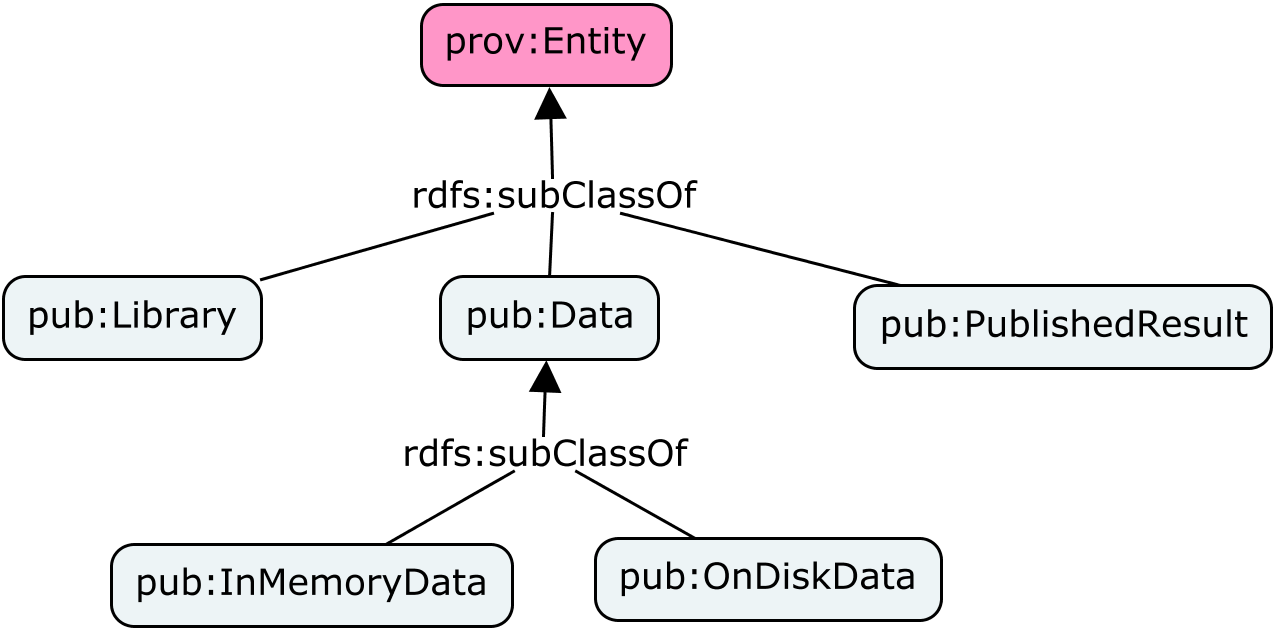
\includegraphics[width=.8\textwidth]{model/ontology/prov-pub/prov-pub-p-entity.png}
	\caption{Entities defined in PROV-PUB-O/P}
	\label{fig:prov-pub-p-entity}
\end{figure}
\begin{figure}
	\centering
	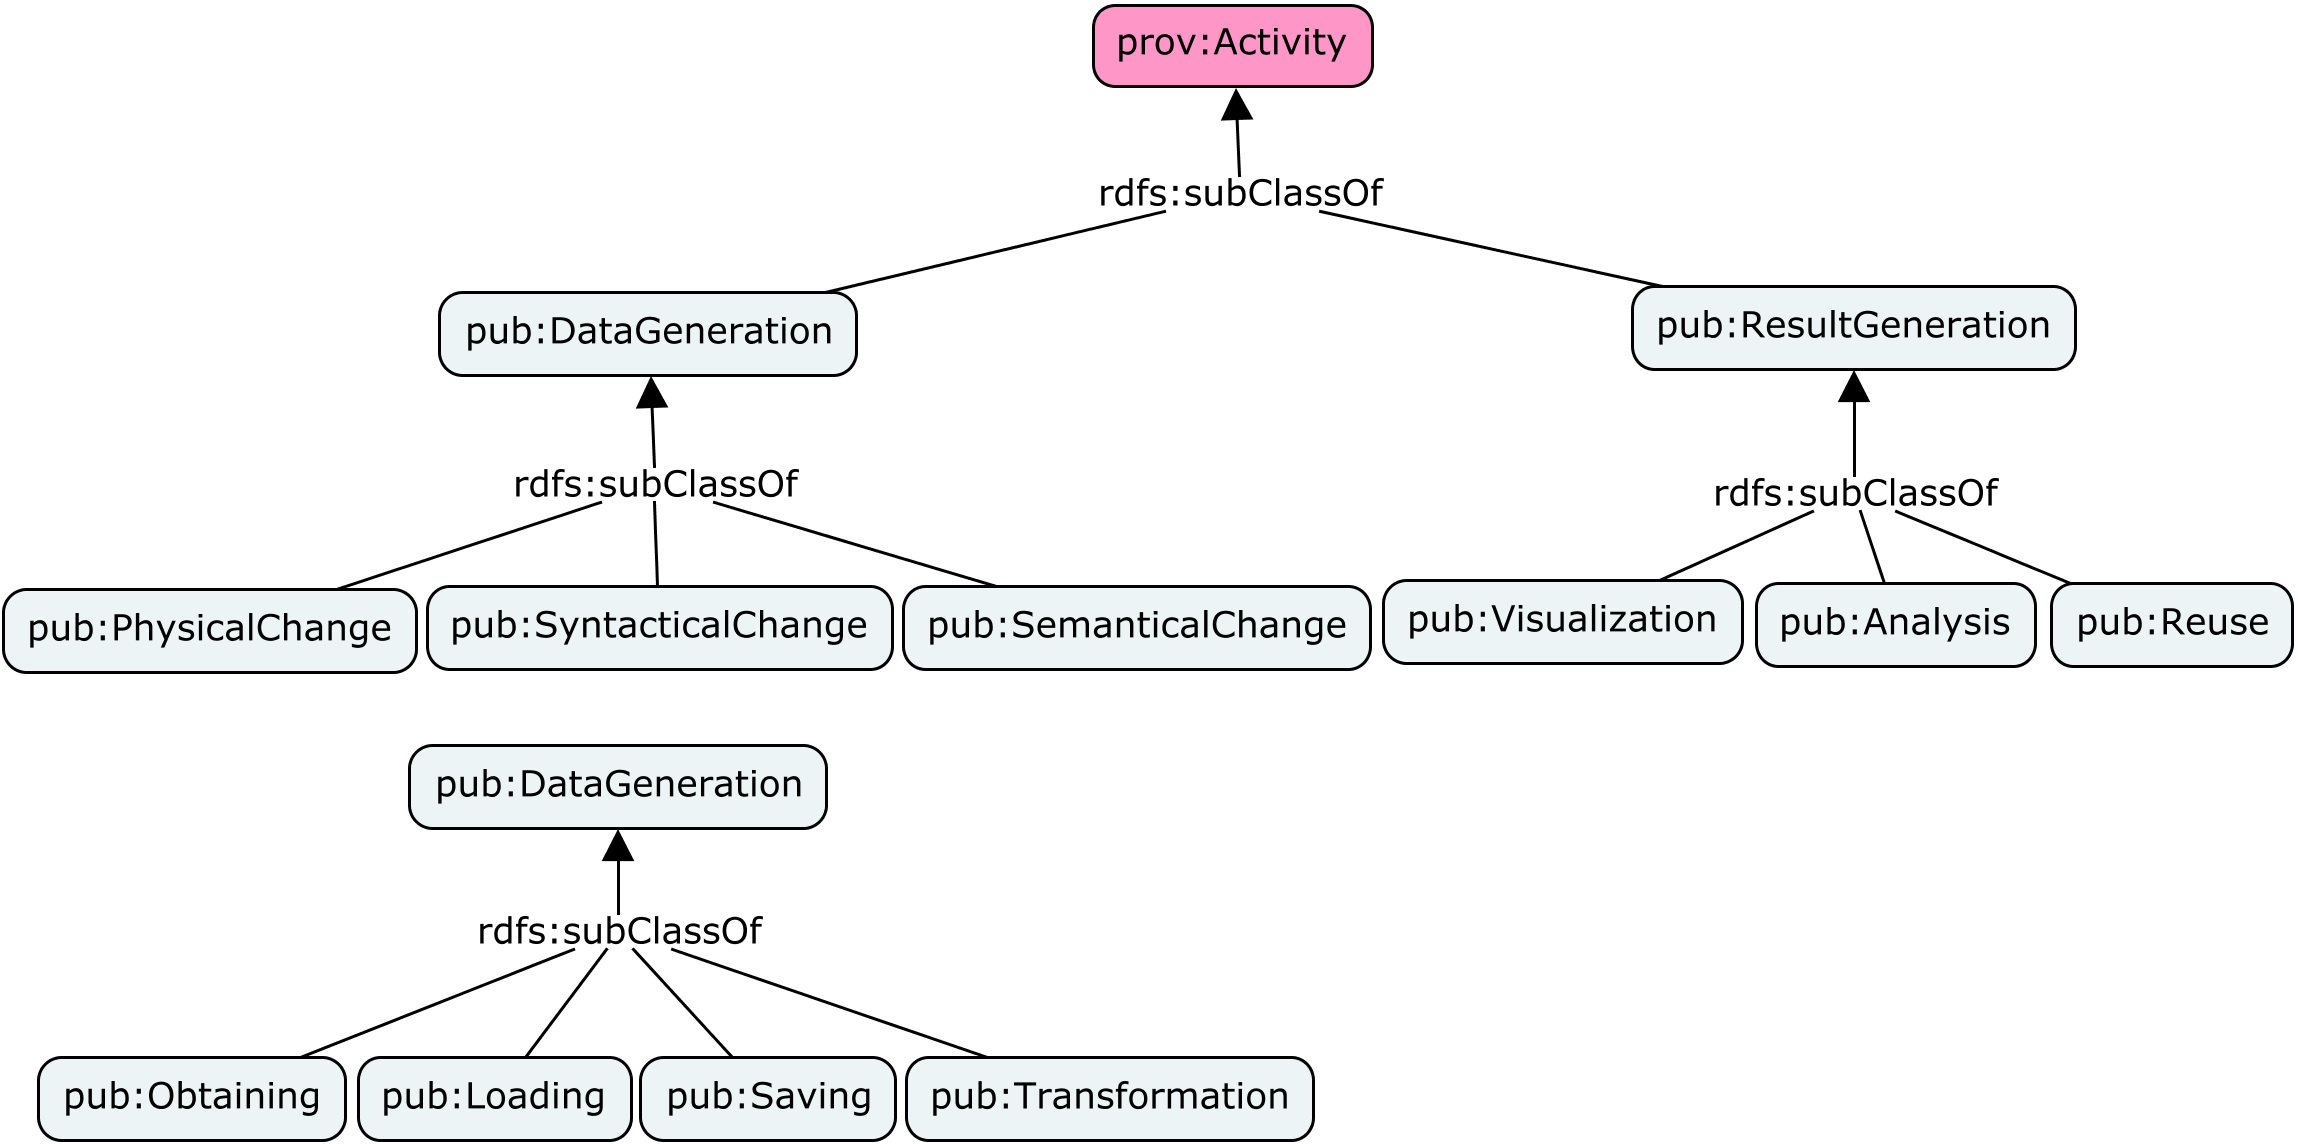
\includegraphics[width=\textwidth]{model/ontology/prov-pub/prov-pub-p-activity.png}
	\caption{Activities defined in PROV-PUB-O/P}
	\label{fig:prov-pub-p-activity}	
\end{figure}

{\noindent\emph{Properties about using data and results:}}
\begin{itemize}
	\item pub:obtained
	\item pub:loaded
	\item pub:saved
	\item pub:transformed%subset slice project filter map...
	\item pub:visualized
	\item pub:analyzed
	\item pub:reused
\end{itemize}
These are sub-properties of prov:used to allow domain-specific ways of describing data and result usage methods. Their names indicate the correspondence between these properties and the data changing and result generation activities mentioned above. For example, pub:obtained is expected to be used with the pub:Obtaining activity. These properties can also be considered ``shortcuts'' to replace the use of prov:qualifiedUsage. For example, the following usage written in PROV-O
\begin{quotation}
:activity1 prov:qualifiedUsage [

  \hspace{2em}prov:entity :data1;
  
  \hspace{2em}dcterms:description "transform"

].
\end{quotation}
could be written in PROV-PUB-O/P as
\begin{quotation}
:activity1 pub:transformed :data1.
\end{quotation}
Figure~\ref{fig:prov-pub-p-usage} shows the sub-properties of prov:used that are defined in PROV-PUB-O/P.
\begin{figure}
	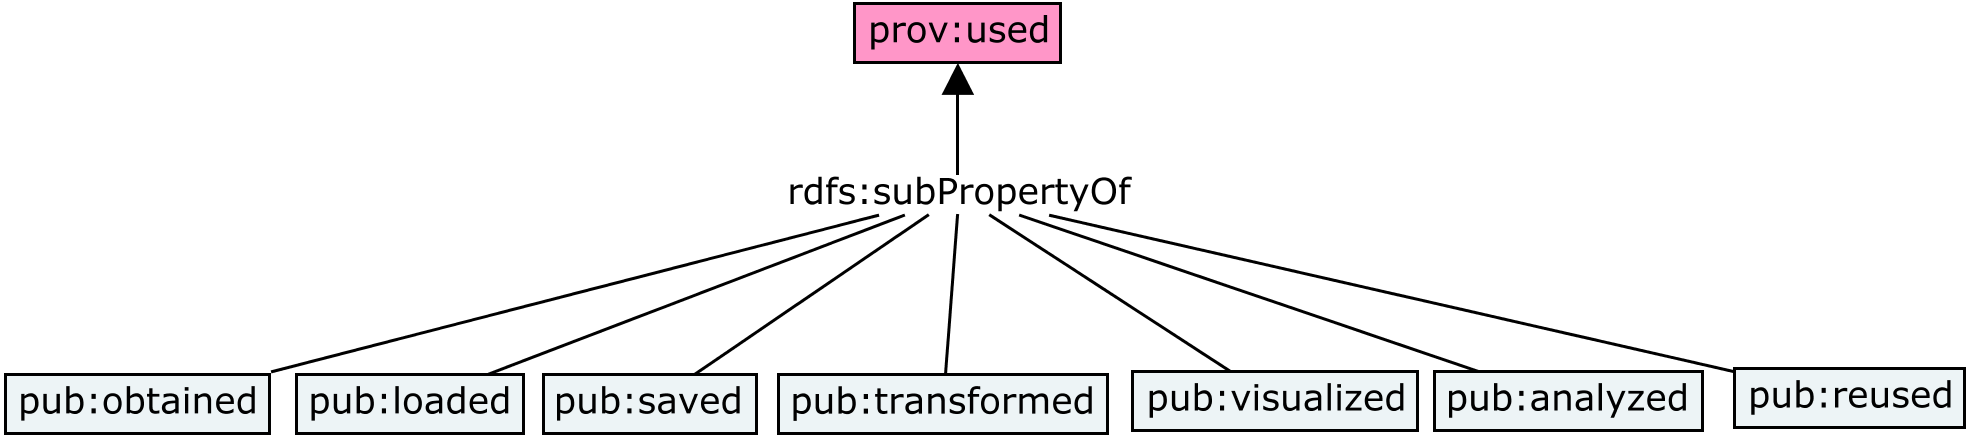
\includegraphics[width=\textwidth]{model/ontology/prov-pub/prov-pub-p-usage.png}
	\caption{Sub-properties of prov:used defined in PROV-PUB-O/P}
	\label{fig:prov-pub-p-usage}
\end{figure}

\noindent\emph{Annotations about change of data and result generation:}
\begin{itemize}
	\item pub:format
	\item pub:language% --- the programming language used in the data changing activity.
	\item pub:code% --- the code in a certain programming language for changing the data. It is recommended that only succinct code that invokes helper functions are included, and the detailed implementation of these helper functions be modeled as pub:Library instances used by data changing activities.
	\item dcterms:description% --- the textual description of the data processing method. 
\end{itemize}
These four annotations are used to describe 1) the format in which on-disk data are, 2) the programming language used in a certain data changing or result generation activity, 3) the code in a certain programming language for changing the data or generating the result and 4) the data processing method in natural language. For the pub:code annotation, it is recommended that only succinct code that invokes helper functions are included, and the detailed implementation code of these helper functions be modeled as pub:Library instances used by the activity in question.

We believe users of PROV-PUB-O/P will benefit from dependencies to PROV-O in forms of subclasses and sub-properties --- after all, this is the very reason we design PROV-PUB-O/P as a specialization of PROV-O --- so we include these assertions in PROV-PUB-O/P.

The specialized ontology is not only helpful in describing the provenance, but it also enables the construction of executable provenance graphs to preserve the data product preparing process at a level that is detailed enough to be replicable.

Figure~\ref{fig:prov-pub-example} shows a sample usage of PROV-PUB-O/P to describe the generation process of a figure very similar with Figure~4.2 in NCA 2014. The obtaining operation, ``:operation0'', generated the on-disk data, ``:csv\_file''. The details of how the data were obtained are described in the textual description, ``dct:description'' of the activity. Then the loading operation, ``:operation1'', loaded the on-disk data into memory as an in-memory data object, ``csv\_content'', which was then transformed by the transformation operation, ``:operation2'', to generate data ``:percent'', which were ready for the visualization operation, ``operation3'', to visualize and generate the published result in the form of a figure: ``:figure4.2''. 

\begin{figure}
	\centering
	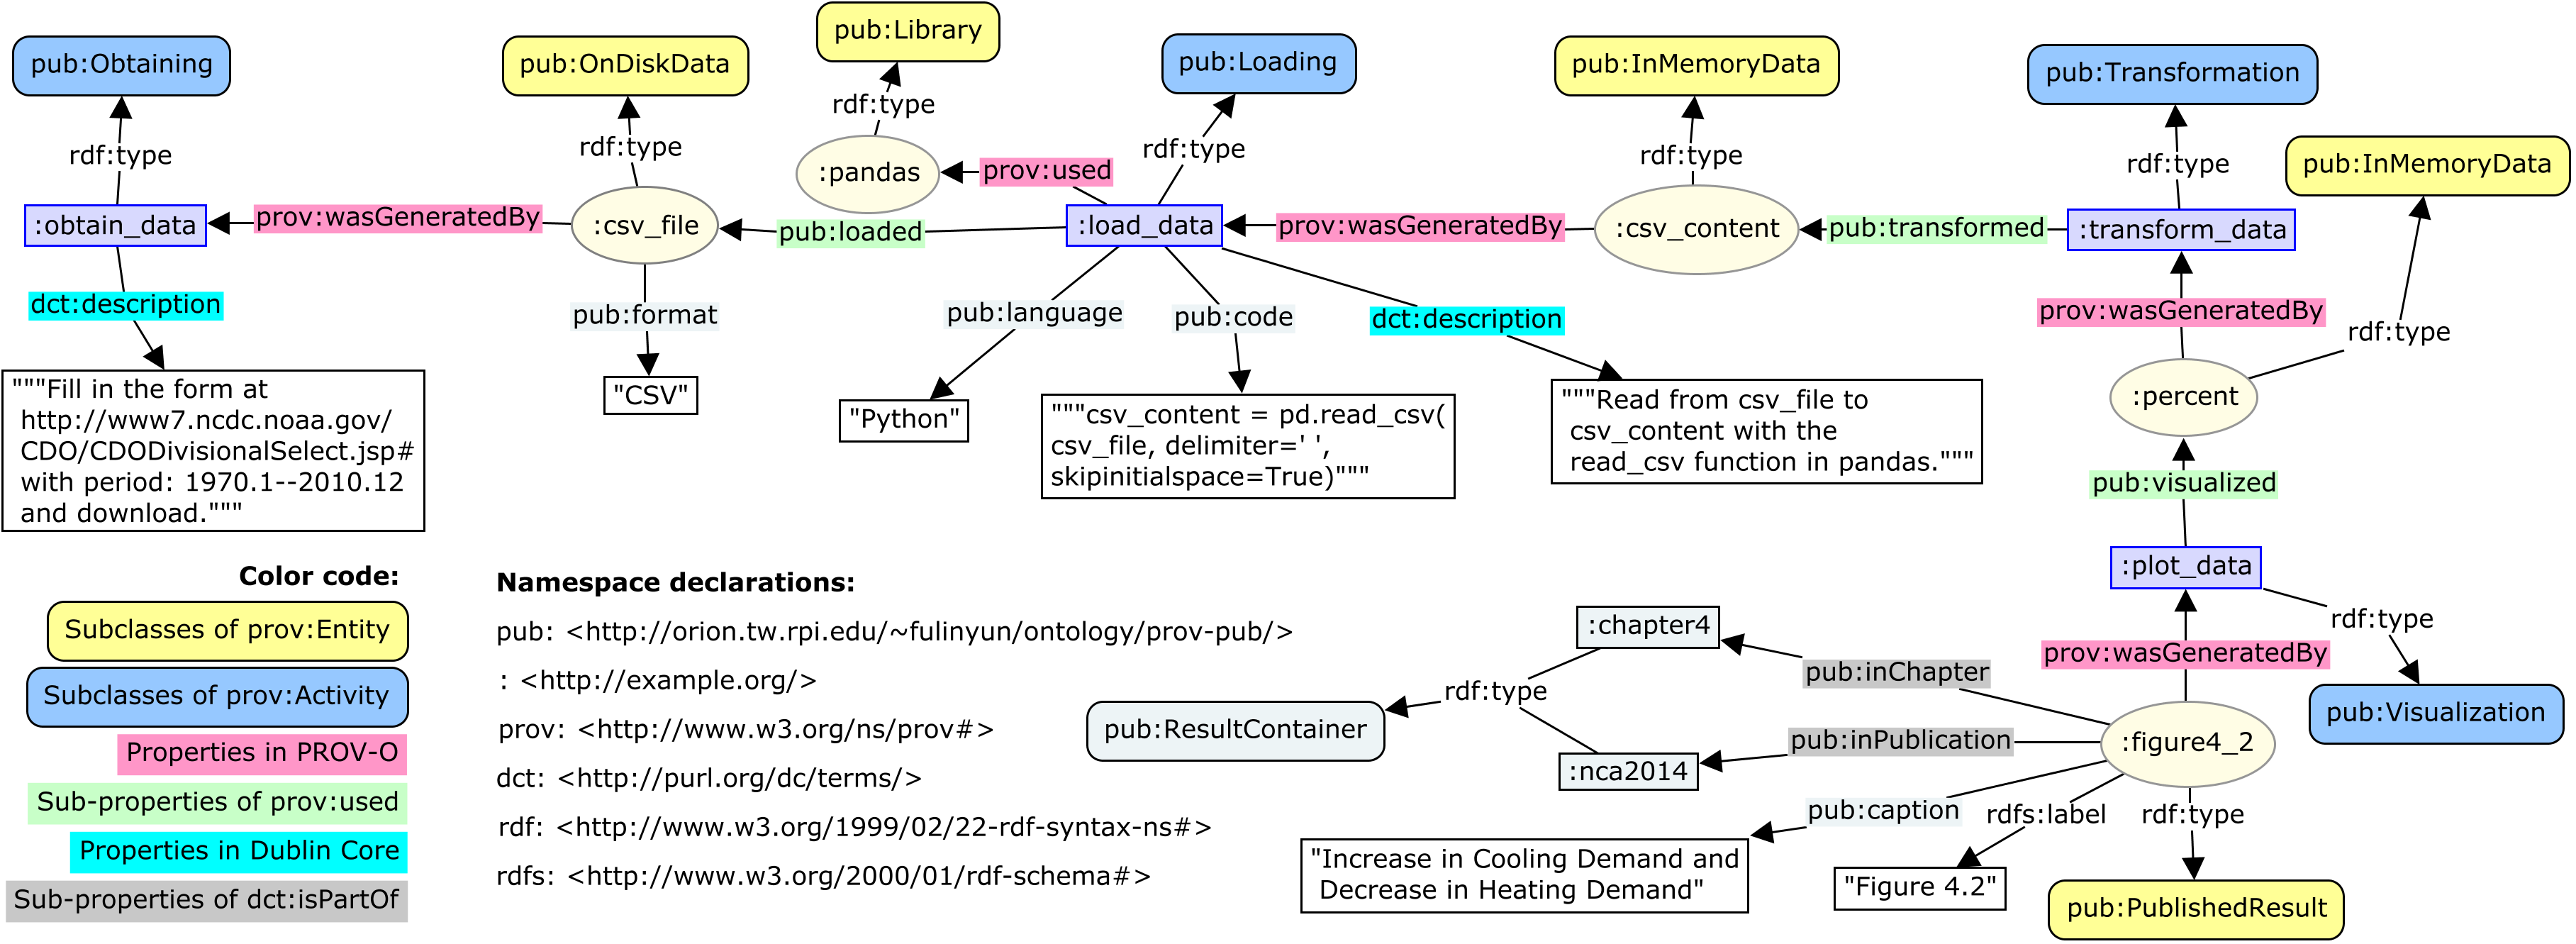
\includegraphics[width=\textwidth]{model/ontology/prov-pub/prov-pub-example.png}
	\caption{Illustrated sample provenance graph in PROV-PUB-O}
	\label{fig:prov-pub-example}
	%\comment{to replace this figure with a more developed one}
\end{figure}

The hypothesis we would like to justify here is that sub-properties of prov:used are more usable than prov:used itself in the use case of creating executable provenance graphs in the domain of earth science.

%\subsubsection{Workflow vs. provenance semantics}

%\subsubsection{Executable provenance graphs}

%\subsubsection{Ontology as software}

\subsection{Ontology usability evaluation approach}
\label{subsec:evaluation}
%\comment{We need to find a recurring scientific data analytics task as our use case. Then analyze the pros and cons of using general and specialized provenance ontologies.}

A substantial part of this section comes from an unpublished article I collaboratively authored with Xiaogang Ma and Patrick West \cite{fu2015ontology}.

% why we need ontology usability evaluation
PROV-PUB-O is a specialization of PROV-O. The goal of such kind of specialization, in general, is to create more usable, rather than more useful, systems. The difference between {\em usefulness} and {\em usability} will be detailed later. Here we provide this example first: some touch screen input keyboard includes a ``.com'' key to make inputting website URLs and email addresses more convenient. Adding the ``.com'' key to the keyboard already containing the ``.'' (dot), ``c'', ``o'' and ``m'' keys does not make it more useful, but more usable. In other words, the keyboard, as an input system, does not get functionally more capable by adding the ``.com'' key, but becomes practically more convenient and pleasant to use for people who need to input dot com website URLs and email addresses belonging to the dot com domain. Note that usability is always related to users with certain tasks to accomplish. For some users, keyboards with a ``.com'' key are more useful than those without, for other users, this may not be true because they never need to input ``.com'': they may instead need to input ``.edu'' a lot, and feel the ``.com'' keyboard the same as the normal one or even cumbersome to use because of the presence of a large but useless key.

% useful and usable
We claim that PROV-PUB-O is more usable to research publication authors than PROV-O. Therefore, to justify that the creation of PROV-PUB-O is indeed a contribution, we need a set of criteria for the evaluation of ontology usability, through which people will be able to describe and assess an ontology from different aspects. The items in the criteria, however, are decided by the understandings about the meaning of \emph{usability}. We adopt the definition given in the international standard ISO 9241-11 \cite{iso19989241}, which has received endorsements from various domains: ``[Usability is] the extent to which a product can be used by specified users to achieve specified goals with effectiveness, efficiency and satisfaction in a specified context of use.'' The background of this definition is Human-Computer Interaction and the definition represents a user-centered point of view \cite{jokela2003standard}. The definition indicates that usability is not about the product itself (or, its quality), but about the activity of a user using it, so usability depends on the goal of the user and the context of the use. With satisfaction as one of its attributes, defined as ``freedom from discomfort, and positive attitude to the use of the product'' \cite{iso19989241}, usability is inevitably subjective.

Therefore, existing criteria for assessing quality of ontologies do not necessarily fit in ontology usability evaluation. Although some of them can serve as strong usability indicators. For example, Gruber \cite{gruber1995toward}
discussed several elements for ontology design: clarity, coherence, extendibility, minimal encoding bias, and minimal ontological commitment, which are all good principles for ontology quality evaluation, but to do usability evaluation, Fox and Lynnes added a few other items, namely contextual relevance, maturity, intended use, and fitness for use, to Gruber's list to cover the contextual and subjective aspects of ontology usability\footnote{Additional items for ontology evaluation. \url{http://tw.rpi.edu/web/project/SeSF/workinggroups/OntologyEvaluation}. Accessed on September 9th, 2015.}.

In this thesis we propose the Ontology Usability Scale (OUS) for the evaluation of ontology usability. The evaluation metrics are reflected in a short list of statements, which were derived from an online poll in the Semantic Web community. We will introduce our thoughts on semiotics when preparing a long list of statements for the poll, and will also analyze the community's concerns on ontology usability by using the outputs of the poll.

\subsubsection{Related work of ontology evaluation}
% history of ontology evaluation.
Although it is hard to find related work specifically on evaluating ontology usability, the general evaluation of ontologies, however, has already received attention even before the introduction of Resource Description Framework (RDF) \cite{brickley2000resource} and Web Ontology Language (OWL) \cite{mcguinness2004owl}. For example, Gr{\"u}ninger et al. \cite{gruninger1995methodology} proposed a method to check the completeness of an ontology with respect to a set of competency questions. Competency questions are the questions that the ontology is designed to answer, so this method checks whether ``the right things are done'', and does not benefit people who later want to reuse the ontology.

%Nowadays many ontologies are written in Resource Description Framework Schema \cite{brickley2000resource} (RDFS) or Web Ontology Language \cite{mcguinness2004owl} (OWL). The evaluation of ontologies, however, has been paid attention to long before the introduction of these two ontology languages. For example, Gr{\"u}ninger et al in their paper \cite{gruninger1995methodology} proposes a method to check the completeness of an ontology with respect to a set of competency questions. Competency questions are the questions that the ontology is designed to answer, so this approach checks whether ``the right things are done''. Back then, ontologies are defined with first-order logic (or equivalently, in Knowledge Interchange Format (KIF)), so the authors formalized competency questions also with first-order logic and evaluate the ontology in question by proving completeness theorems with respect to these formal competency questions.

With the major Semantic Web standards and heavily reused upper ontologies being available (see Figure~\ref{fig:timeline} for a timeline of Semantic Web standards, and \cite{bikakis2013xml} for the details), representing domain knowledge with ontologies became a common practice and it became more and more likely to see several different conceptualizations of the same domain. Therefore, ontology evaluation methods for the purpose of selecting and reusing existing ontologies for new applications were greatly needed.

\begin{figure}
	\centering
	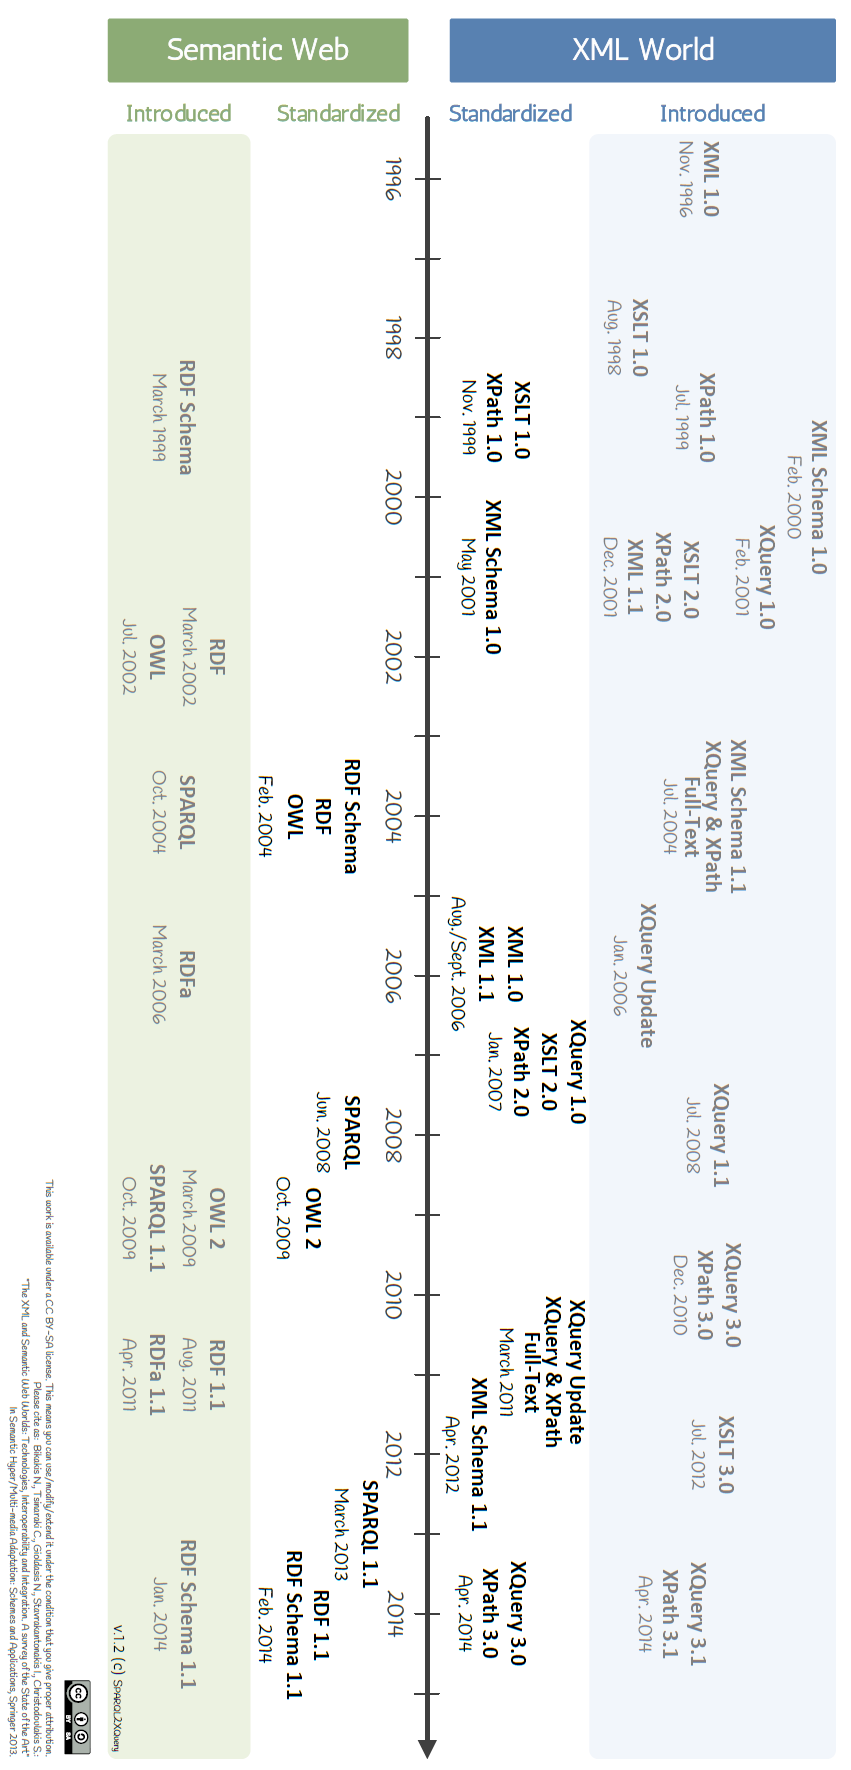
\includegraphics[width=\linewidth]{XMLSemanticWebW3CTimeline}
	\caption[XML and Semantic Web W3C Standards Timeline]{XML and Semantic Web W3C Standards Timeline}
	\label{fig:timeline}
\end{figure}

A popular approach to do this kind of evaluation is to define several criteria for decision making, evaluate the ontology in question on each criterion by giving a numerical score, and then compute the overall score for the ontology as a weighted sum of the per-criterion scores. Such methods are called multiple-criteria approaches in \cite{brank2005survey}. For example, Fox et al. \cite{fox1995organisation} proposed a set of criteria including generality, completeness, perspicuity, and so on. Gomez-Perez in her paper \cite{gomez2001evaluation} published in 2001 pointed out the lack of interest in evaluation issues in the ontological engineering community at that time. She also pointed out that tools, tutorials and case studies are critical for ontology engineers to assess the usability of an existing ontology. Nevertheless, the paper does not give an example of ontology usability evaluation, it instead evaluates the Standard-Unit Ontology in terms of consistency, completeness and conciseness, so the evaluation result is not directly related to the effectiveness, efficiency and satisfaction of the users when they reuse a certain ontology. An ontology may be consistent (i.e. without any contradictory assertion), complete (i.e. without any missing definition) and concise (i.e. without any unnecessary definition), but still be unusable or very cumbersome to use (e.g. due to bad documentation).

Lozano-Tello et al. presented the ONTOMETRIC method \cite{lozano2003selection,lozano2004ontometric}, which compares ontologies with a taxonomy of 160 characteristics organized in a multi-level tree-shaped framework. At the top level, there are five basic aspects. These are: 
\begin{enumerate}
	\item the \emph{content} of the ontology and the
	organization of their contents, 
	\item the \emph{language}
	in which it is implemented, 
	\item the \emph{methodology}
	that has been followed to develop it,
	\item the software \emph{tools} used to build and edit
	the ontology, and 
	\item the \emph{costs} that the ontology
	will be necessary in a certain project.
\end{enumerate}
The final score for an ontology is calculated as the weighted sum of the scores given to each of the leaf node characteristics, through aggregations at each of the internal nodes governing aspects and sub-aspects of the ontology characteristics. It could be imagined that the scoring and weight assignment would take a lot of time and be easily biased by the viewpoint of the scorer, as pointed out by Hartmann et al. in \cite{hartmann2005d1}. Similar with ONTOMETRIC, our approach also requires a scorer to get a single numerical score for each ontology in question, but we provide the scorer a Likert scale (a questionnaire asking for degrees of agreement with a list of statements) consisting of around 10 items, instead of a huge scoring form with pending weights for each item. We found a small portion of the 160 characteristics directly related to usability, and drew them out as our candidate usability metrics.

%As more and more ontologies became available online (see Figure~\ref{fig:timeline} for a timeline of Semantic Web standards, and \cite{bikakis2013xml} for the details), attention is paid to the evaluation of ontologies for the purpose of selecting an existing ontology to reuse in a new application. A popular way to do this kind of evaluation is to define several criteria for decision making, evaluate the ontology in question on each of them, giving a numerical score, and compute the overall score for the ontology as a weighted sum of its per-criterion scores. This group of approaches is called \emph{multiple-criteria approaches} in \cite{brank2005survey}. For example, Fox et al in \cite{fox1995organisation} proposed a set of criteria including \emph{generality}, \emph{completeness}, \emph{perspicuity}, etc.; G{\'o}mez-P{\'e}rez in her paper \cite{gomez2001evaluation} published in 2001 pointed out the lack of interest in evaluation issues in the ontological engineering community at that time. She also pointed out that tools, tutorials and case studies are critical for ontology engineers to assess the usability of an existing ontology. Unfortunately the paper does not give an example of ontology usability evaluation, it instead evaluates the Standard-Unit Ontology in terms of consistency, completeness and conciseness; Lozano-Tello et al present the \emph{ONTOMETRIC} method \cite{lozano2003selection,lozano2004ontometric}, which compares ontologies with a taxonomy of
%160 characteristics organized in a multilevel framework. At the top level, there are five basic aspects. These are: the \emph{content} of the ontology and the
%organization of their contents, the \emph{language}
%in which it is implemented, the \emph{methodology}
%that has been followed to develop it,
%the software \emph{tools} used to build and edit
%the ontology, and the \emph{costs} that the ontology
%will be necessary in a certain project. For each ontology under consideration, the ONTOMETRIC method basically calculates the weighted sum of the scores given to each of the leaf node characteristics of this tree-shaped framework. Aggregated scores are obtained for sub-tree roots as the calculation ascending each level along the tree, so the final score is finally available at the root node. Hartmann et al in \cite{hartmann2005d1} pointed out the following two usability issues of ONTOMETRIC:
%\begin{itemize}
%	\item Specifying the characteristics of an ontology
%	is complicated and takes time
%	\item Assessing
%	the characteristics is quite subjective (from the
%	project managers' viewpoint)
%\end{itemize} 

Different from the studies mentioned above, Burton-Jones et al. \cite{burton2005semiotic} proposed a set of 10 attributes that fall into four metrics suites (i.e. syntactic, semantic, pragmatic and social quality) of a semiotic frame-work. They tried to find objective indicators to assess each recognized metric to eliminate the need of human reviewers. For example, the \emph{Lawfulness} dimension of the \emph{Syntax} metric is indicated by the percentage of correct syntax per class and property. The authors suggested that the evaluation could be extended to cover application-centered assessment of the quality of an ontology for use in a specific task. We create our list of candidate usability metrics by thinking in the aspects of syntax, semantics and pragmatics. We assume that the difference of social quality (authority and history) between two ontologies would dwarf the
overall impact of these three other aspects. In fact, only ontologies of similar social quality are worth comparing. If one of them has significantly more authority (i.e. more ontologies rely on it) or longer history (i.e. it has been used more), it would be an obvious winner. We also found it hard, if not impossible, to assess some of the important metrics with objective indicators. For example, the quality of documentation is very important to the usability of the ontology, but it is hardly possible to be measured in any objective way, so we argue that it requires the participation of human reviewers to get meaningful usability assessments.

%Different from the studies mentioned above, Burton-Jones et al proposed a set of 10 objective metrics at 4 different levels of a semiotic framework in \cite{burton2005semiotic}. Their work supports objective evaluation of ontologies, which does not require experts' review of the ontologies in questions. 

The semiotic framework was also used in Gangemi et al. \cite{gangemi2006qood}. The authors organized the criteria for ontology evaluation and selection with a semiotic meta-ontology called $O^2$ and the oQual evaluation ontology which involves concepts and relations relevant to ontology evaluation and selection. Therefore, evaluation based on the oQual ontology goes beyond the mere calculation of a weighted sum, but also contains reasoning based on the evaluation ontology. Goals of reusing the ontology and trade-off rules among conflicting goals must be defined formally and in a way that connects with $O^2$ and oQual in order to follow their approach, which limits its application to ontology experts only. The target user group of our metrics is anyone who wants to select an ontology suitable to an application (meaning the user can apply the selected ontology to his/her use case with the most aggregated effectiveness, efficiency and satisfaction among all the candidate ontologies), so we require much less ontological expertise of our users than their approach.

%In \cite{gangemi2006qood}, Gangemi et al organized the criteria for ontology evaluation and selection with a semiotic meta-ontology called $O^2$ and the \emph{oQual} evaluation ontology which involves concepts and relations relevant to ontology evaluation and selection. Therefore, evaluation based on the oQual ontology goes beyond the mere calculation of a weighted sum, but also contains reasoning based on the evaluation ontology. 
%\comment{to read: OntoQA \cite{tartir2005ontoqa} (schema- and instance- level metrics) Ontology metrics design \cite{vrandevcic2007design} Unit tests for ontologies \cite{vrandevcic2006unit}.} 

Casellas \cite{casellas2009ontology} used System Usability Scale \cite{brooke1996sus} to evaluate the usability of the Ontology of Professional Judicial Knowledge (See Chapter 2 of \cite{casellas2009ontology} for an introduction of the ontology). Our approach differs with Casellas' in how we select the statements in the questionnaire. Casellas directly tailored the 10 items in SUS, but we think that the set of statements that best indicate the usability of ontologies may need to consider more aspects. We created a pool of 29 candidate statements by adapting several resources, including those used in \cite{casellas2009ontology}. Then we built the usability scale from those candidate statements through some community efforts, i.e. we gathered preferences among the Semantic Web community through an online poll. The result of the poll verified our thoughts since it differed a lot from the statement set in \cite{casellas2009ontology}.

\subsubsection{Research approach for creating OUS}
The intuition behind our approach to evaluating ontology usability comes from the System Usability Scale (SUS), a ten-item Likert scale whose usage is recommended by the UsabilityNet project as ``it is very robust and has been extensively used and adapted. Of all the public domain questionnaires, this is the most strongly recommended''. We hope to have such a concise scale that is applicable for ontology usability evaluation.

A direct adaptation of SUS for ontology (i.e. replace ``system'' with ``ontology'' in the questionnaire) does not cover all the aspects in our understanding of the ontology usability. Therefore, besides those items adapted from SUS, we collected usability evaluation statements from ONTOMETRIC \cite{lozano2004ontometric} and Casellas' work \cite{casellas2009ontology} to set up a large pool of statements. When collecting those statements we also refer to the semiotic framework discussed in Burton-Jones et al. \cite{burton2005semiotic} and Gangemi et al. \cite{gangemi2006qood}, but our understanding of the syn-tax, semantics and pragmatics is slightly different because in our work the focus is the usability. We consider syntax is relevant to the machine readable encoding and logic of the content of an ontology; semantics is relevant to the conceptual model and documentation; and pragmatics is relevant to the first hand experience of using the ontology in practice. Table~\ref{tab:statements-pool} shows the grouped statements in the large pool. Note that we changed some statements originally in negative forms to positive forms so that all the statements are desired features of a highly usable ontology. Each feature represented by one of the statements can be represented in either the positive form or the negative form. Both forms are found in our original statement set. Two of these statements, numbered 23 and 26 in Table~\ref{tab:statements-pool}, are even in the two forms of exactly the same feature. To eliminate bias caused by the statement representation form and avoid listing the same feature twice (in both positive and negative forms) in the questionnaire, we decided to normalize every statement to its positive form.

\begin{longtable}{p{\textwidth}}
	\caption{The large pool of statements for ontology usability evaluation}
	\label{tab:statements-pool}\\
	\hline
	Syntax (Content)
	\begin{enumerate}
		\item I found the various concepts in this ontology well integrated
		\item The ontology misses some important concepts --- Changed to ``The ontology has all the important concepts included'' in the survey
		\item The ontology has unnecessary concepts --- Changed to ``The ontology does not have unnecessary concepts''
		\item I found the ontology unnecessarily complex --- Changed to ``I found the ontology brief but comprehensive''
		\item I thought there was too much inconsistency in this ontology --- Changed to ``I found the various parts of this ontology well integrated''
		\item I found the formal specification of concepts in this ontology coincides with their descriptions in natural language
		\item I found the formal specification of relations in this ontology coincides with their descriptions in natural language
		\item I think the attributes in this ontology describe the concepts well
		\item I think the relations in this ontology relate appropriate concepts
		\item I found the subclasses in this ontology are properly defined
		\item I found the disjoint classes in this ontology are properly asserted
	\end{enumerate} \\
	\hline
	Semantics (Documentation)
	\begin{enumerate}
		\setcounter{enumi}{11}
		\item The purpose of this ontology is clear
		\item I am confident I understand the conceptualization of the ontology
		\item I need to ask a lot of questions before I could understand the conceptualization of the ontology --- Changed to ``I could understand the conceptualization of the ontology without asking a lot of questions''
		\item I find the ontology easy to understand
		\item The annotations are helpful
		\item I found the concepts in this ontology properly described in natural language
		\item I found the relations in this ontology properly described in natural language
		\item I need further theoretical support to understand this ontology --- Changed to ``I do not need further theoretical support to be able to understand this ontology''
		\item I would imagine that most domain experts would understand this ontology very quickly
	\end{enumerate} \\
	\hline
	Pragmatics (First-hand experience)
	\begin{enumerate}
		\setcounter{enumi}{20}
		\item I would imagine that most people would learn to use this ontology very quickly
		\item I needed to learn a lot of things before I could get going with this ontology --- Changed to ``I do not need to learn any extra things before I could get going with this ontology''
		\item I thought the ontology was easy to use
		\item It is clear to me how to use this ontology
		\item I felt very confident using the ontology
		\item I found the ontology very cumbersome to use --- Deleted in the survey since it is the negative form of statement 23 and we decided to present all the statements in their positive forms only.
		\item I think that I would need the support of a person experienced with this ontology to be able to use it --- Changed to ``I do not need the support of a person experienced with this ontology to be able to use it''
		\item I need some more examples than provided in the documentation to make sure how to use the ontology --- Changed to ``I think the documentation provides sufficient examples for me to make sure how to use the ontology''
		\item I think that I would like to use this ontology frequently
		\item I think that I could contribute to this ontology
	\end{enumerate} \\
	\hline
\end{longtable}
The long list of statements can help provide a comprehensive usability evaluation, but the burden caused by the number of statements can be an issue, so we reached out to the semantic web community to ask for a poll for selecting 10 representative statements. We sent out invitations to the semantic web working group of the Federation of Earth Science Information Partners, the semantic web group on Facebook, and also colleagues at Tetherless World Constellation at Rensselaer Polytechnic Institute. To avoid confusion in reading the statements, we changed the forms of a few of them (see notes in Table~\ref{tab:statements-pool}) to make all the statements have a positive form, i.e. towards the goodness of an ontology instead of shortcomings. Moreover, we mixed the sequence of those statements in the survey and did not show the three groups of syntax, semantics and pragmatics of those statements in order to avoid any bias that may be led to the survey participants. We received 18 valid responses in 7 days, and the top 11 statements from the poll and the votes they each received are shown in Table~\ref{tab:poll}.
\begin{table}
	\centering
	\caption{The top 11 statements resulted from an online poll and the votes to each statement received}
	\label{tab:poll}
	\begin{tabular}{|p{0.06\textwidth}|p{0.62\textwidth}|p{0.13\textwidth}|p{0.06\textwidth}|}
		\hline Num-ber & Statement & Category & Votes \\ 
		\hline 1 & I think the documentation provides sufficient examples for me to make sure how to use the ontology. & Pragmatics & 14 \\ 
		\hline 2 & The purpose of this ontology is clear. & Semantics & 9 \\ 
		\hline 3 & I found the concepts in this ontology properly described in natural language. & Semantics & 9 \\ 
		\hline 4 & I think the relations in this ontology relate appropriate concepts. & Syntax & 8 \\ 
		\hline 5 & I am confident I understand the conceptualization of the ontology. & Semantics & 8 \\ 
		\hline 6 & I would imagine that most domain experts would understand this ontology very quickly. & Semantics & 7 \\ 
		\hline 7 & I think the attributes in this ontology describe the concepts well. & Syntax & 7 \\ 
		\hline 8 & I found the subclasses in this ontology are properly defined. & Syntax & 7 \\ 
		\hline 9 & I found the relations in this ontology properly described in natural language. & Semantics & 7 \\ 
		\hline 10 & I found the formal specification of concepts in this ontology coincides with their descriptions in natu-ral language. & Syntax & 7 \\ 
		\hline 11 & I do not need the support of a person experienced with this ontology to be able to use it. & Pragmatics & 7 \\ 
		\hline 
	\end{tabular} 
\end{table}
In Table~\ref{tab:poll} we can see that 5 of the top 11 statements are about semantics, 4 for syntax and the left 2 for pragmatics, which is a strong indication that usability of ontology is mostly about semantics and syntax. This also supports our above discussion that the SUS probably would not work well on ontologies because it is mostly about pragmatics.

We compiled our 10-item Likert scale for ontology usability evaluation based on the above result, as shown in Table~\ref{tab:ous-draft}.
\begin{table}
	\begin{center}
		\caption{Ontology usability evaluation questionnaire (draft)}
		\label{tab:ous-draft}
		\begin{tabular}{|p{0.1\textwidth}|p{0.62\textwidth}|l|l|l|l|l|}
			\hline Number & Statement & 1 & 2 & 3 & 4 & 5 \\ 
			\hline 1 & I think the documentation provides sufficient examples for me to make sure how to use the ontology. &  &  &  &  &  \\ 
			\hline 2 & The purpose of this ontology is clear. &  &  &  &  &  \\ 
			\hline 3 & I found the concepts and relations in this ontology properly described in natural language. &  &  &  &  &  \\ 
			\hline 4 & I think the relations in this ontology relate appropriate concepts. &  &  &  &  &  \\ 
			\hline 5 & I am confident I understand the conceptualization of the ontology. &  &  &  &  &  \\ 
			\hline 6 & I would imagine that most domain experts would understand this ontology very quickly. &  &  &  &  &  \\ 
			\hline 7 & I think the attributes in this ontology describe the concepts well. &  &  &  &  &  \\ 
			\hline 8 & I found the subclasses in this ontology are properly defined. &  &  &  &  &  \\ 
			\hline 9 & I found the formal specification of concepts and relations in this ontology coincides with their descriptions in natural language. &  &  &  &  &  \\ 
			\hline 10 & I do not need the support of a person experienced with this ontology to be able to use it. &  &  &  &  &  \\ 
			\hline 
		\end{tabular} 
	\end{center}
\end{table}
In Table~\ref{tab:ous-draft}, closely related statements about concepts
and relations were merged together. i.e., statements
3 and 9 in Table~\ref{tab:poll} were merged to ``I found the
concepts and relations in this ontology properly described
in natural language'', and statement 10 was
changed to ``I found the formal specification of concepts
and relations in this ontology coincides with
their descriptions in natural language''. We did this
based on the assumption that concepts are equally
important as and considered together with relations
in an ontology.

A scale from 1 to 5 was used to indicate ``highly
disagree'', ``disagree'', ``neutral'', ``agree'' and ``highly
agree'' against each statement in Table 3, so higher
scores mean better usability. To assess the usability
of an ontology using this form, a scorer needs to give
a score indicating his/her degree of agreement for
each statement, denoted as $s_1$, $s_2$, ..., $s_10$, then the
total score $s_t$ is calculated as
\begin{equation}
\label{eq1}
s_t = \sum_{i=1}^{10}s_i
\end{equation}
, which ranges from 10 to 50.

To further improve the questionnaire, we use positive
and negative forms of statements in Table~\ref{tab:ous-draft} alternately
to make scorers more attentive when they
fill out the form. The adapted and reorganized statements
are shown in Table~\ref{tab:ous}.
\begin{table}
	\centering
	\caption{Recommended ontology usability scale}
	\label{tab:ous}
		\begin{tabular}{|p{0.1\textwidth}|p{0.62\textwidth}|l|l|l|l|l|}
			\hline Number & Statement & 1 & 2 & 3 & 4 & 5 \\ 
			\hline 1 & The purpose of this ontology is clear. &  &  &  &  &  \\ 
			\hline 2 & I need more examples than provided in the documentation to make sure how to use the ontology. &  &  &  &  &  \\ 
			\hline 3 & I found the concepts and relations in this ontology properly described in natural language. &  &  &  &  &  \\ 
			\hline 4 & There is inconsistency between the formal specification of concepts and relations in this ontology and their descriptions
			in natural language. &  &  &  &  &  \\ 
			\hline 5 & I would imagine that most domain experts would understand this ontology very quickly. &  &  &  &  &  \\ 
			\hline 6 & I think that I would need the support of a person experienced with this ontology to be able to use it. &  &  &  &  &  \\ 
			\hline 7 & I am confident I understand the conceptualization of the ontology. &  &  &  &  &  \\ 
			\hline 8 & The attributes in this ontology fail to describe the concepts properly. &  &  &  &  &  \\ 
			\hline 9 & I think the relations in this ontology relate appropriate concepts. &  &  &  &  &  \\ 
			\hline 10 & I think the class hierarchy of this ontology needs better organization. &  &  &  &  &  \\ 
			\hline 
		\end{tabular} 
\end{table}
In Table~\ref{tab:ous}, the statements at odd numbered positions
are all in a positive form and those at even
numbered positions are all in a negative form. To use
this form, Equation~\ref{eq1} needs to be changed to
\begin{equation}
\label{eq2}
s_t = \sum_{i \textrm{ \scriptsize is odd}}s_i+\sum_{i \textrm{ \scriptsize is even}}(6-s_i)
\end{equation}
, which still ranges from 10 to 50. A higher score
indicates a higher usability.
\subsubsection{Case study and evaluation}
We used the developed OUS, i.e. statements in
Table~\ref{tab:ous} for a case study of ontology usability evaluation
within the Tetherless World Constellation at
Rensselaer Polytechnic Institute. The case study was
carried out as an anonymous online survey, in which
each participant was asked to choose an ontology and
assign a score to each statement. The outputs of the
survey are listed in Table~\ref{tab:ous}. Since revisions are currently
undergoing to update the ontologies of Deep Carbon Observatory (DCO) and Global Change In-formation System (GCIS), we will be able to apply the developed OUS to their later versions to check if the revisions are effective in terms of usability. Comparisons among ontologies with similar intended uses and different versions of the same ontology are made easy with OUS since each ontology is given an overall score calculated from the answers given by each reviewer. Scoring an OUS form (Table~\ref{tab:ous}) does not require much of the reviewers' time, but the collected answers provide simple yet comprehensive assessments of the usability of the ontologies in question.
\begin{table}
	\centering
	\caption{Results of ontology usability evaluation in a case study}
	\label{tab:ous-case}
	\begin{tabular}{|l|l|l|l|l|l|l|l|l|l|l|l|}
		\hline Ontology & $s_1$ & $s_2$ & $s_3$ & $s_4$ & $s_5$ & $s_6$ & $s_7$ & $s_8$ & $s_9$ & $s_{10}$ & $s_t$ \\ 
		\hline DCO & 5 & 4 & 3 & 2 & 4 & 3 & 5 & 2 & 4 & 2 & 38 \\ 
		\hline DCO & 5 & 4 & 4 & 1 & 3 & 2 & 5 & 1 & 5 & 2 & 42 \\ 
		\hline DCO & 3 & 1 & 4 & 3 & 2 & 2 & 2 & 4 & 3 & 5 & 29 \\ 
		\hline GCIS & 4 & 2 & 4 & 2 & 4 & 3 & 4 & 2 & 4 & 3 & 38 \\ 
		\hline GCIS & 5 & 3 & 4 & 1 & 5 & 2 & 5 & 1 & 5 & 3 & 44 \\ 
		\hline SIO & 5 & 5 & 5 & 2 & 5 & 5 & 2 & 1 & 5 & 3 & 36 \\ 
		\hline VSTO & 1 & 5 & 1 & 3 & 2 & 4 & 4 & 2 & 4 & 2 & 26 \\ 
		\hline 
	\end{tabular} 
\end{table}

\subsubsection{Discussion on OUS}
The resulting ontology usability scale of this study covers topics of syntax, semantics and pragmatics and addresses the issue of evaluating the usability of an ontology in a certain context. The list of statements in the current scale (Table~\ref{tab:ous}) is based on a survey. It has a concise structure and is easy to use in practice. The scale can be used by all stakeholders who participated in the development, application, and revision of an ontology, and the result can be used to improve the ontology.

Semiotics is the study of signs. It is applicable to ontologies because ontologies are sign systems to represent knowledge. The division of semiotics into semantics, syntactics and pragmatics was contributed by Morris \cite{morris1938foundations}. According to Morris, semantics is the study of the relation of signs to the things they refer to (their designata); syntactics is the study of the relation of signs to one another; pragmatics studies the relation of signs to their interpreters. In the case of ontology, we define semantics as the mapping of domain knowledge to ontological elements such as classes and relations, or the meaning of these elements, conveyed through the conceptual model and documentation. Syntactics (or syntax according to Burton-Jones et al. \cite{burton2005semiotic}) is defined as the way the ontological elements are organized, usually with terms in RDFS or OWL. Pragmatics is the relation of ontologies to their users, so it is about the activity of a user using an ontology.

According to the above definitions, it seems only the pragmatical dimension of semiotics is relevant to ontology usability since it is the only dimension about the ontology using activity rather than the ontology itself, and usability is about certain attributes of the activity of using a certain product rather than attributes of the product itself according to ISO 9241-11 \cite{iso19989241}. However, unlike simple signs which their users interpret out of intuition and experience, ontological terms require users to learn their semantical and syntactical features in order to interpret, typically through learning the term organization and reading the documentation. Therefore, all the three dimensions of semiotics are relevant to ontology usability. In fact, the survey result shown in Table~\ref{tab:poll} even indicated that the semantical and syntactical aspects may be more important than the pragmatical aspect, since only 2 out of the 11 top selections fall in the pragmatics group.

ISO 9241-11 \cite{iso19989241} listed the following three aspects of usability, \emph{effectiveness} is about accuracy and completeness of the result of that activity, \emph{efficiency} is the resources expended during the process, such as time and effort of learning and creating solutions, and \emph{satisfaction} is the freedom from discomfort and the positive attitude towards the use of the product. As we tried to decide which semiotical aspect impact which usability aspect, we found that each semiotical aspect may impact every usability aspect. For example, missing or insufficiently illustrated ontological terms (semantical aspect) may cause the user unable to complete his or her tasks (effectiveness), to spend more time learning the conceptualization (efficiency), and/or to feel discomfortable (satisfaction). Inconsistent or counter-intuitive organization of the ontological elements (syntactical) may have the same effect in terms of effectiveness, efficiency and satisfaction, and the pragmatical aspect aligns well with the overall usability. Therefore, the semiotical aspects and the usability aspects are closely related, so it is reasonable to classify usability criteria with semiotical aspects.

The survey result brings feedbacks and inspirations to ontology developers. As indicated by the top selections in Table~\ref{tab:poll}, stating the purpose of the ontology explicitly, describing classes and relations in detail and providing abundant examples in the documentation will greatly help users understand and use the ontology. The purpose of an ontology is important probably because of the close relationship between usability and purpose. Usability is inherently associated with fitness, and fitness, as summed up by Terry Pratchett in his novel ``Moving Pictures'', means ``appropriateness to a purpose'' \cite{pratchett2005moving} (quoted by Brooke in \cite{brooke1996sus}). Besides the statements pool in Table~\ref{tab:statements-pool}, in the online survey we also invited participants to write down any additional statements from their point of view. One suggestion is about the provenance of components in an ontology, such as the cited source in the definition of a class or property, and the person who asserts the definition, etc. Another issue is about the serialization language of ontologies. It was mentioned that if an ontology is not serialized in a simple format such as Turtle, it can be difficult for a user to read and understand. Another participant proposed the issue of ontology maintenance/sustainability, such as the stability of the ontology over time and the level of maintenance support that the ontology has. In \cite{ma2013recent} Ma et al. discussed that to achieve better ontology applications, people need to balance the expressivity, implementability and maintainability of the ontology. The maintainability or sustainability is relevant to the usability of an ontology in a long term period.

In the online survey we also received active feedbacks about the organization and form of the statements. In the survey preparation we tried to group the statements into three categories following a semiotic framework, while in the survey we did not show the groups and listed the statements in a random order. Our intention is to avoid any bias that may be caused by those pre-defined groups. It was interesting to see that several participants suggested the statement pool should be categorized, especially from the point of view of an ontologist. Another participant suggested that there can be a separation of statements for subject matter experts and end users.

Survey participants also commented on the positive and negative forms of the statements. From the comments we could see that it is okay to use both forms in a questionnaire, but we should avoid duplicated statements, such as ``I thought the ontology was easy to use'' and ``I found the ontology very cumbersome to use.'' Considering those feedbacks, we organized two sets of statements for ontology usability evaluation in Table~\ref{tab:ous-draft} and Table~\ref{tab:ous}, one with only statements in positive form and the other with both positive and negative forms.
Besides the top 11 mostly voted statements in Table~\ref{tab:poll}, we also took a review of the least voted statements in the online poll (Table~\ref{tab:least}). Most of them have either an extreme or vague meaning. Statement 1 in Table~\ref{tab:least} is adapted from its negative form ``I needed to learn a lot of things before I could get going with this ontology''; statement 2 was originally ``The on-tology has unnecessary concepts''; statement 3 overlaps a lot in meaning with ``I found the concepts/relations in this ontology properly described in natural language'' but is less clear; statement 4 is very similar to ``I would imagine that most domain experts would understand this ontology very quickly'', and statement 5 similar to ``I found the various concepts in this ontology well integrated'' (which was selected 4 times).
\begin{table}
	\centering
\caption{The least voted statements in the online poll}
\label{tab:least}
\begin{tabular}{|p{0.09\textwidth}|p{0.6\textwidth}|p{0.13\textwidth}|p{0.06\textwidth}|}
	\hline Number & Statement & Category & Votes \\ 
	\hline 1 & I do not need to learn any extra things before I could get going with this ontology. & Pragmatics & 0 \\ 
	\hline 2 & The ontology does not have unnecessary concepts. & Syntax & 2 \\ 
	\hline 3 & The annotations are helpful. & Semantics & 2 \\ 
	\hline 4 & I would imagine that most people would learn to use this ontology very quickly. & Pragmatics & 2 \\ 
	\hline 5 & I found the various parts of this ontology were well integrated. & Syntax & 2 \\ 
	\hline 
\end{tabular} 
\end{table}

We also collected information about what ontologies the surveyees had worked with, the top ones are shown in Table~\ref{tab:ontologies}.
\begin{table}
	\centering
\caption{Ontologies that the online surveyees worked with}
\label{tab:ontologies}
\begin{tabular}{|l|l|}
	\hline Ontology & Number of people worked with it \\ 
	\hline SWEET & 11 \\ 
	\hline Dublin Core & 8 \\ 
	\hline FOAF & 7 \\ 
	\hline SKOS & 5 \\ 
	\hline PROV-O & 3 \\ 
	\hline GCIS & 3 \\ 
	\hline 
\end{tabular} 
\end{table}
We found that users of domain ontologies such as SWEET have different preferences on statements from users of general ontologies such as Dublin Core. Top 12 selections for SWEET users listed in Table~\ref{tab:sweet} are very similar with those in Table~\ref{tab:poll}, with only a few minor differences. For example, statement 6 in Table~\ref{tab:poll} (``I would imagine that most domain experts would understand this ontology very quickly'') is missing in Table~\ref{tab:sweet}, but it ranks 13th among SWEET users; statement 10 and 12 in Table~\ref{tab:sweet} is missing in Table 2, but they rank 12th and 13th among all the statements so did not make it to the top 11 in Table~\ref{tab:poll}.
\begin{table}
	\centering
\caption{Top 12 statements selected by SWEET users}
\label{tab:sweet}
\begin{tabular}{|l|p{0.7\textwidth}|l|}
	\hline Number & Statement & Votes \\ 
	\hline 1 & The purpose of this ontology is clear. & 8 \\ 
	\hline 2 & I think the documentation provides sufficient examples for me to make sure how to use the ontology. & 8 \\ 
	\hline 3 & I think the relations in this ontology relate appropriate concepts. & 7 \\ 
	\hline 4 & I found the concepts in this ontology properly described in natural language. & 6 \\ 
	\hline 5 & I am confident I understand the conceptualization of the ontology. & 6 \\ 
	\hline 6 & I think the attributes in this ontology describe the concepts well. & 5 \\ 
	\hline 7 & I found the subclasses in this ontology are properly defined. & 5 \\ 
	\hline 8 & I do not need the support of a person experienced with this ontology to be able to use it. & 5 \\ 
	\hline 9 & I found the relations in this ontology properly described in natural language. & 4 \\ 
	\hline 10 & I found the ontology brief but comprehensive. & 4 \\ 
	\hline 11 & I found the formal specification of concepts in this ontology coincides with their descriptions in natural language. & 4 \\ 
	\hline 12 & I find the ontology easy to understand. & 4 \\ 
	\hline 
\end{tabular} 
\end{table}
But among the top three selections by Dublin Core users shown in Table~\ref{tab:dc}, two of them (``I think that I would like to use this ontology frequently'' and ``It is clear to me how to use this ontology'') are missing in Table~\ref{tab:poll}, so for ontologies designed to be used across different domains, statements 2 and 3 in Table~\ref{tab:dc} could be added to the usability scale.
\begin{table}
	\centering
	\caption{Top 3 statements selected by Dublin Core users}
	\label{tab:dc}
	\begin{tabular}{|l|p{0.7\textwidth}|l|}
		\hline Number & Statement & Votes \\ 
		\hline 1 & I think the documentation provides sufficient examples for me to make sure how to use the ontology. & 7 \\ 
		\hline 2 & I think that I would like to use this ontology frequently. & 5 \\ 
		\hline 3 & It is clear to me how to use this ontology. & 4 \\ 
		\hline 
	\end{tabular} 
\end{table}
There are several issues that can be explored in future works. The first work is to have more case studies using the statements in Table~\ref{tab:ous-draft} and Table~\ref{tab:ous}. In this study we only carried out case studies of the ontology usability scale in the GCIS and the DCO projects. Although the feedbacks are positive, we want to hear more feedbacks and suggestions on the statements themselves, including both their forms and the orders, as well the topics covered. The second potential work is relevant to the ontology types. As Table~\ref{tab:ontologies} shows, among the ontologies that the survey participants had worked with, there are both upper ontologies (e.g. Dublin Core, PROV-O) and domain ontologies (e.g. SWEET, GCIS). The former are applicable across a range of domain and the latter are only used for a specific application or domain. Therefore, we may organize corresponding statements for the usability evaluation of those two types of ontologies, and we can take further surveys to see if there are any differences between the community's concerns on the two ontology types. In the current survey we did not ask the participants to specify their roles and experiences in the ontology work. The third potential work is that, if we are going to have new surveys, we can ask people about their roles (e.g. ontology developer, database curator, application developer, and so on.) and their experience with ontology use (e.g. number of years). Last, the fourth potential work is to enrich, update and reorganize the statement pool from the point of view on expressivity, implementability and maintainability of ontologies. This framework is slightly different from the semiotic framework on syntax, semantics and pragmatics and covers new aspects of ontology usability.

\section{Automatic provenance capturing framework}
In computer science, a framework is a parameterized system. Certain components of the framework could be customized to fulfill specific tasks. The proposed provenance capturing framework in this thesis consists of the following components:
\begin{itemize}
	\item A \emph{platform} is the managing system that coordinates its front end, operators and store. 
	\item The \emph{front end} of the platform is the interface for the users to interact with the platform. It provides the users ways to input requests to the platform that could be fulfilled with certain operators. Usually a platform kernel, which is a special operator, interprets user actions into requests and forwards these requests to the platform. The front end also takes feedback from the operators of the platform after they finish processing requests and interprets it into user-friendly feedback to display to the users. A front end could be as simple as a line processor that deals with one line of input text in each round of interaction with the user, but it could also be as capable as a system monitor that receives every single event happened on the user interface of the operating system. For such capable front end, users could interact with it in ways far beyond inputting commands and looking at textual feedback. For example, a user could open a browser and download a file, in which case the front end will take the sequence of events and interpret it into something the platform kernel understands, such as a ``download file'' command.
	\item The \emph{operators} of the platform are provenance aware software tools or scripts that execute operations on data and record provenance at each execution time. They can be included in the platform as pre-installed utilities but users are expected to obtain new operators for new tasks from time to time. The front end and the platform kernel (if there exists one) does not necessarily know the operational logics of a certain operator but must know how to invoke the operator according to the requests from the users and how to receive feedback from the operator.
	\item The \emph{kernel} of the platform is an optional special operator that directly interact with the front end. It deals with all the requests interpreted by the front end either itself or through dispatching to other operators. If there is a kernel in the platform, it must be the only operator that directly interact with the front end, and all the other operators must only interact with the kernel operator. In this thesis we focus on the case where there is a kernel. One important job of the kernel is to assign consistent URIs to the data objects across different operations. We will go to the details of this point in Section~\ref{sec:transition}.
	\item The \emph{store} of the platform takes charge of temporarily holding in-memory provenance fragments and storing provenance on disks. For a platform compliant with PROV-PUB-O, its store is equivalent with an RDF graph in the vocabulary of PROV-PUB-O.
\end{itemize}
The front end will invoke operators when the user launches a command through the front end. Operations on data are then delegated to various operators and execution results are sent back to the front end to enable it to provide meaningful feedback to the user. Execution of operations may require accesses to the store to operate in-memory or on-disk data objects. These processes are illustrated in Figure~\ref{fig:invoke} and Figure~\ref{fig:execute}.
\begin{figure}
	\centering
	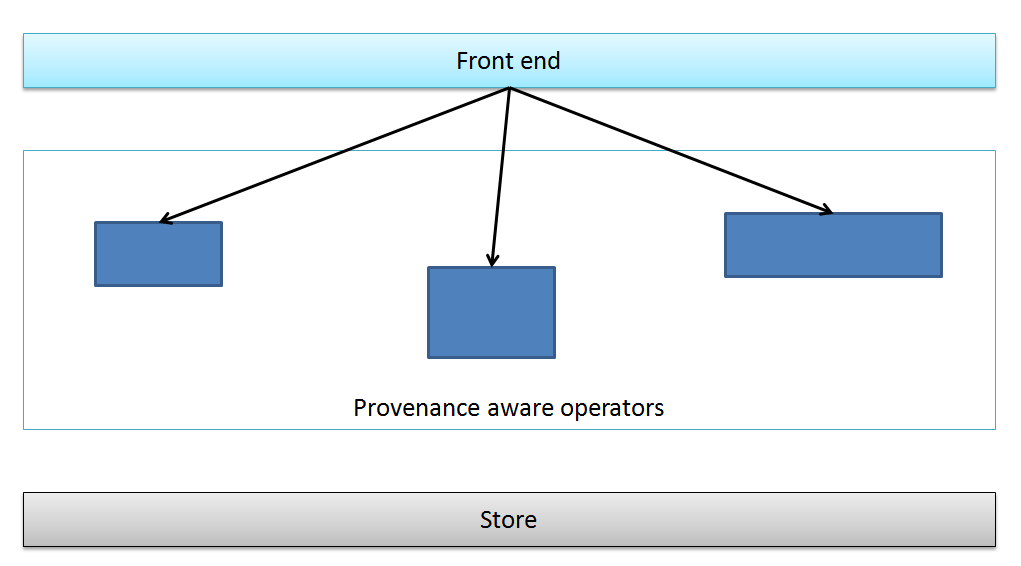
\includegraphics[width=\textwidth]{invoke.png}
	\caption{Front end invoke operators to finish tasks}
	\label{fig:invoke}
\end{figure}
\begin{figure}
	\centering
	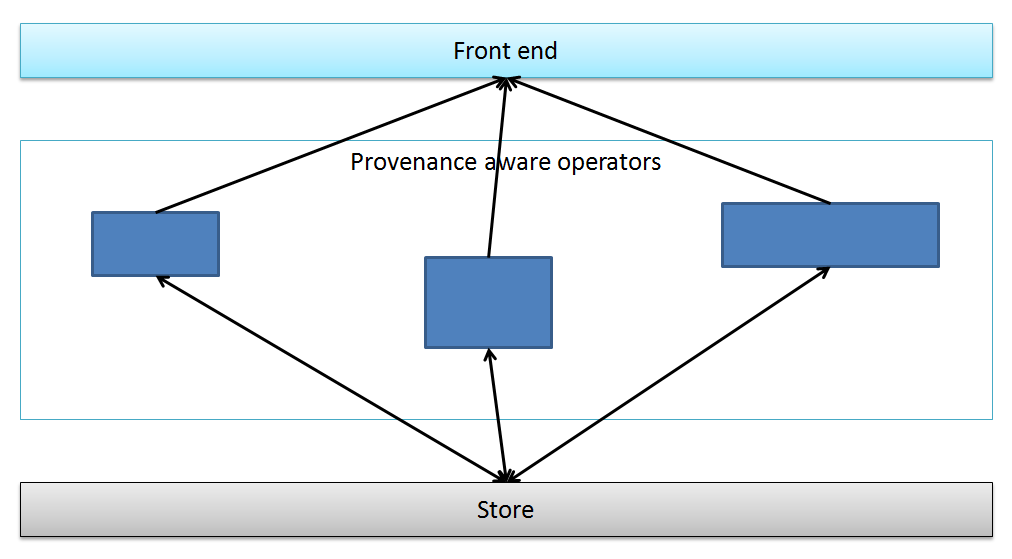
\includegraphics[width=\textwidth]{execute.png}
	\caption{Operators access store and notify front end}
	\label{fig:execute}
\end{figure}
An important feature of the platform is that the front end and the store both only interact with operators, as shown in Figure~\ref{fig:platform}.
\begin{figure}
	\centering
	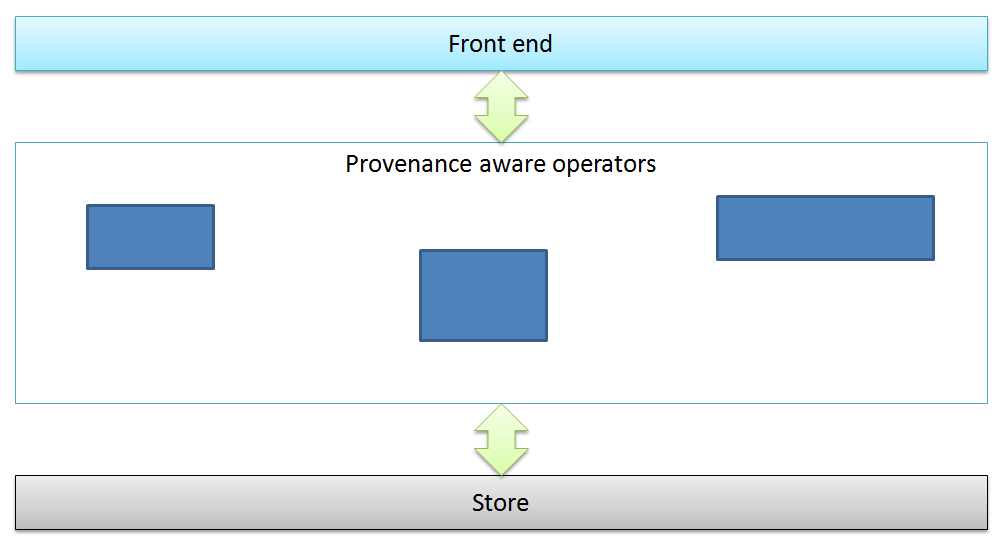
\includegraphics[width=\textwidth]{platform.png}
	\caption{Front end and store both only interact with operators}
	\label{fig:platform}
\end{figure}
A corollary of this feature, is that the creation and retrieving of provenance should be on those operators, rather than the front end or the store. Because if the operators do not create provenance, the store has no way to get provenance since it only interacts with operators. Provenance would then get lost because it has to be saved in the store. Operators must be able to retrieve provenance for the readers of the research publications to reproduce the published results because only they have access to the store, where provenance is kept.

Since neither the front end nor the platform kernel necessarily know the operational logic of every possible operator they are to invoke for some task, it is impossible to implement the provenance capturing function as part of the front end or platform kernel. For example, an operator may use several data objects to generate multiple other data objects. Some of these objects may be passed as parameters of function calls, others may be defined as the return values, and positions of these objects (whether they are parameters or return values) could be arbitrarily decided by the developer of the operator (software or scripts), so the job of creating and retrieving provenance has to be done by the operators. In the case where a kernel exists, it has the job of connecting provenance fragments generated within other operators. For example, an operator O1 used data D1 as one of its arguments and generated data D2 as its return value. In this case the operator O1 knows what D1 and D2 are but does not know the identities of D1 and D2 within the context where O1 gets invoked. In other words, O1 knows D1 is the $n$-th argument, and D2 the return value, but O1 has no way to know which variable is holding its $n$-th argument and which variable will hold its return value. The kernel operator knows where each argument comes from and where each return value goes to, so it has to be involved in provenance capturing to assign consistent URIs to data objects and results.

Provenance collecting frameworks proposed before the publication of PROV-O such as \cite{simmhan2006framework} must depend on a central provenance service to collect provenance graph fragments provided by the various components operating on data to ensure these fragments are consistent with each other and can be put together to form the whole provenance graph. With PROV-PUB-O/P, which is a specialization of PROV-O, such a centralized provenance authority just need to simply concatenate the lists of triples generated by the operators, as long as all the operators format their provenance pieces with the same terminology. This assumption holds given that there is a terminology to be used that has been publicly published and widely adopted.

The two functions of the platform, namely the creation of provenance and the replication of the research work with the saved provenance, do not have big differences between them. The only difference is that the replication requires an additional ``load provenance'' operation at the very beginning.

\subsection{System state transition rules}
\label{sec:transition}
Given a front end, a finite set of operators including the kernel, and a store, the platform becomes a system. The state of the system gets changed only when one of the following events happens:
\begin{itemize}
	\item The system gets started.
	\item One operation gets executed by a certain operator.
	\item The system is closed.
\end{itemize}
Of these three events, the first and the third does not require special attention in terms of provenance capturing. At the start-up time of the system, the store just needs to be initialized to an empty graph, and at the ending time of the system, the store needs to be saved to disk.

\subsubsection{What operation means}
Before we focus on the second event, we want to make clear what does ``an operation'' mean. In this thesis, an operation must have the following abstract form:
\begin{equation}
\label{eq:fun}
\textrm{function}(\textrm{argument1}, \textrm{argument2}, \dots, \textrm{argumentN})\rightarrow \textrm{return}
\end{equation}
The meaning of this operation is that a function of an operator with N arguments is invoked to generate a return. Note that through simple wrapping, logical and arithmetic operations can be converted to this form. For example, x plus y gets z could be written as a function ``plus'' taking two arguments x and y, and generating z:
\begin{equation}
\textrm{plus}(x, y)\rightarrow z
\end{equation}
We do not allow the function to change some of its arguments as a side effect, this demand could be fulfilled by rewriting the function definition to move these arguments to the return side, in which case the return would have these changed arguments all held in some data structure such as a list or a dictionary.

Here we follow the kernel language approach described in Chapter 2.3 of the book written by Peter Van Roy and Seif Haridi~\cite{van2004concepts}. Table 2.1 in this chapter summarizes all the basic operations needed by a general programming language, thus these operations must be sufficient for creating results in research publications.

In fact, the kernel language defined in Table 2.1 in \cite{van2004concepts} could be redefined as in Table~\ref{tab:kernel}. 
\begin{table}
	\centering
	\begin{tabular}{|rrll|}
		\hline $<s>$ & ::= & skip & Empty statement \\ 
		  & | & $<s>_1$ $<s>_2$ & Statement sequence \\ 
		  & | & $<x>_2\rightarrow <x>_1$ & Variable binding \\ 
		  & | & $<v>\rightarrow<x>$ & Value assignment \\ 
		  & | & $f(<a>_1\dots<a>_n)\rightarrow r$ & Operation invocation \\ 
		\hline 
	\end{tabular} 
	\caption{Kernel language adapted from Van Roy and Haridi's work}
	\label{tab:kernel}
\end{table}
The differences are:
\begin{itemize}
	\item Variable creation and binding are in one step (this is the case for functional programming languages, and is adopted by Python and R), so there is no separate variable creation step.
	\item Procedure applications are replaced by operation invocations. To convert a procedure application to an operation invocation, we just need to move those arguments that would be changed to the return value side (the $r$ side).
	\item Conditional and pattern matching statements are removed, they must be written in the form of operation invocations.
\end{itemize}
In fact, variable binding and value assignment could also be written in the form of operation invocations. Thus the program could be further simplified to just a sequence of operation invocations: variable binding could be rewritten as the kernel operation ``bind($<x>_2$)$\rightarrow <x>_1$'', and value assignment could be written as ``assign($<v>$)$\rightarrow <x>$''. Therefore, $<x>_2\rightarrow <x>_1$ and $<v>\rightarrow<x>$ could be seen as the syntactical sugar provided by certain kernels. Certain kernels could allow conditional statements and pattern matching statements and many more conveniences implemented in this manner. That is, they are actually operation invocations to the kernel.

\subsubsection{Operation invocation rules}
For the event of an operation gets executed by a certain operator, if the operator is the kernel, then the kernel will generate a fresh URI for the operation, and the operation will be asserted to be an instance of a certain class in PROV-PUB-O according to the kernel's knowledge about the operation (for example, the kernel may assert the operation to be a pub:Obtaining, or a pub:Loading, and so on). The data objects used among the operation's arguments will be recorded with proper sub-properties of prov:used, that is, pub:obtained, pub:loaded, and so on. These data objects will get fresh URIs generated by the kernel. Finally, the fact of the operation generating the returned data object will also be recorded as a triple in the store.

For example, suppose the read\_csv(input\_file)-->csv\_content operation is handled directly by the kernel, then the following triples will be added to the store once this operation gets executed:
\begin{itemize}
	\item (:read\_csv, rdf:type, pub:Loading)
	\item (:read\_csv, pub:loaded, :input\_file)
	\item (:read\_csv, prov:generated, :csv\_content)
	\item (:read\_csv, dct:description, ``Read data in CSV format from the input\_file to the csv\_content object.'')
\end{itemize}
The pub:language and pub:code properties of :read\_csv can also be provided according to specific kernel configurations.

Note that URIs such as :read\_csv, :input\_file and :csv\_content could be replaced with any fresh URIs not yet been used by other data objects.

These provenance capturing actions are taken in addition to the normal actions performed by the platform.

A kernel usually provides only the most basic operations such as value assignment, variable binding, logic and arithmetic operations, and conditional execution. More complicated computations are typically carried out by some provenance aware operator other than the kernel. In this case, the kernel knows the variable carrying the return value of the operation and all the arguments that could potentially be used by the operation, but it does not know the detailed usage of these arguments, neither does the kernel know the specific type of the operation. The operator needs to fill in the blanks where the kernel does not know about it.

For example, suppose the read\_csv(input\_file)$\rightarrow$csv\_content operation is handled by a provenance aware operator instead of the kernel, the same list of triples need to be generated:
\begin{itemize}
	\item (:read\_csv, rdf:type, pub:Loading)
	\item (:read\_csv, pub:loaded, :input\_file)
	\item (:read\_csv, prov:generated, :csv\_content)
	\item (:read\_csv, dct:description, ``Read data in CSV format from the input\_file to the csv\_content object.'')
\end{itemize}
All the fresh URIs for read\_csv, input\_file and csv\_content must be provided by the kernel, the kernel will pass the dictionary of variable-URI mappings to the operator. The operator knows the relationships among these data objects, so it is responsible to generate all the triples with the URIs provided by the kernel. It can also generate more triples that describe useful information such as the programming language and the library dependency.

Note that when generating URI for read\_csv, the URI is not for the function, but for the particular invocation of the function read\_csv, so later invocation of the same function will need different fresh URIs to differentiate among the different function invocations. The same rule holds for different references of the same data object generated at different occasions. Since the internal value changed, they are considered different data objects and need different URIs. Data objects on the left hand side of the operations (arguments of the operations) are considered ``read only'', so they should reuse their existing URIs if such URIs have been created for them.

\subsection{A comprehensive example}
Suppose we have the following list of operations:
\begin{enumerate}
	\item obtain\_data()$\rightarrow$input\_file
	\item read\_csv(input\_file)$\rightarrow$csv\_content
	\item transform\_data(csv\_content)$\rightarrow$plot\_ready\_data
	\item save\_data(plot\_ready\_data)$\rightarrow$data\_file
	\item plot\_data(plot\_ready\_data)$\rightarrow$figure
\end{enumerate}
, and they are all carried out by non-kernel operators. Below is a step-by-step illustration of how each operation should change the store. It shows the minimum set of triples every implementation of the framework needs to generate.

Step 1: obtain\_data()$\rightarrow$input\_file. The kernel is responsible for parsing the operation, and generating fresh URIs :obtain\_data and :input\_file for the invocation of the obtain\_data() operation and the generated data object input\_file, respectively. The operator providing the obtain\_data function is responsible for generating the following triples based on the URIs given by the kernel to add to the store:
\begin{itemize}
	\item (:obtain\_data, rdf:type, pub:Obtaining)
	\item (:obtain\_data, prov:generated, :input\_file)
\end{itemize}
Optionally it may also generate the following triple to explain the obtaining process:
\begin{itemize}
	\item (:obtain\_data, dct:description, "Filled out the data request form at \url{http://www7.ncdc.noaa.gov/CDO/CDODivisionalSelect.jsp#} with period: 1970.1--2010.12, and downloaded the requested data.")
\end{itemize}
and the following triple to describe the obtained data:
\begin{itemize}
	\item (:input\_file, rdf:type, pub:OnDiskData)
	\item (:input\_file, pub:format, "CSV")
	\item (:input\_file, dct:description, "Data in the CDODiv2177686828992.txt file.")
\end{itemize}
The operator may also describe the dataset it obtained data from, with some other ontology focusing on dataset description.

Step 2: read\_csv(input\_file)$\rightarrow$csv\_content. The kernel is responsible for parsing the operation, and generating fresh URIs :read\_csv and :csv\_content for the operation and the generated data object, respectively. The URI for input\_file should be reused because it has not changed from when generated until it is passed as an argument of this operation. The provider of the read\_csv operation is responsible for generating the following triples:
\begin{itemize}
	\item (:read\_csv, rdf:type, pub:Loading)
	\item (:read\_csv, pub:loaded, :input\_file)
	\item (:read\_csv, prov:generated, :csv\_content)
\end{itemize}
Optionally, the operator may also generate some explanation text for the data loading activity:
\begin{itemize}
	\item (:read\_csv, dct:description, "Read CSV data in file CDODiv2177686828992.txt to variable csv\_content")
\end{itemize}
The file name is known by the operator since it is included in the input\_file argument. The variable name needs to be passed by the kernel to the operator. As will be shown in Section~\ref{sec:prototype}, at least in Python, there is a way to pass such ``hidden arguments'' in the background without bothering the user with mysterious additional arguments.

The operator providing the read\_csv function may also provide additional description triples for the :input\_file data object from a different perspective from the data obtaining operator. In this case there is no such additional description to add.

Finally, the operator may provide description for the :csv\_content data object:
\begin{itemize}
	\item (:csv\_content, rdf:type, pub:InMemoryData)
	\item (:csv\_content, dct:description, "Data held by variable csv\_content.")
\end{itemize}

Step 3: transform\_data(csv\_content)$\rightarrow$plot\_ready\_data. The kernel should prepare fresh URIs for the transform\_data operation and the plot\_ready\_data object (let's say they are :transform\_data and :plot\_ready\_data), and reuse the existing URI for the csv\_content object (that is, :csv\_content). The operator should generate the following triples:
\begin{itemize}
	\item (:transform\_data, rdf:type, pub:Transformation)
	\item (:transform\_data, pub:transformed, :csv\_content)
	\item (:transform\_data, prov:generated, :plot\_ready\_data)
\end{itemize}
and it may optionally generate description of the operation:
\begin{itemize}
	\item (:transform\_data, dct:description, "Sum up values on columns CDD and HDD for each year, convert these sums into percentages relative to the average of the first 31 years, delete the remaining columns.")
\end{itemize}
In this example, the transform\_data operation is very problem specific and not useful to other use cases. In the real life, as will be shown in Section~\ref{sec:prototype}, such data transformation is usually decomposed into several general operations such as selecting certain columns (also called subsetting, slicing, and so on), calculating the average for a certain list of values, arithmetic calculation for each value in a list, and so on. Here we put these transformations together as one to avoid listing too many examples of the same kind of data generation operation and to make one complete example of the whole data processing workflow.

The operator providing the transform\_data function may provide additional description of the csv\_content data object according to its knowledge about it. We omit it here. Finally, the operator may generate some triples to describe the data object it generated:
\begin{itemize}
	\item (:plot\_ready\_data, rdf:type, pub:InMemoryData)
	\item (:plot\_ready\_data, dct:description, "Data held by variable :plot\_ready\_data.")
\end{itemize}

Step 4: save\_data(plot\_ready\_data)$\rightarrow$data\_file. Same URI generation jobs are to be done by the kernel. :save\_data for the operation and :data\_file for the generated data object should be ready after kernel does its job. :plot\_ready\_data should get reused. Based on these data object-URI mappings, the operator should generate the following triples:
\begin{itemize}
	\item (:save\_data, rdf:type, pub:Saving)
	\item (:save\_data, pub:saved, :plot\_ready\_data)
	\item (:save\_data, prov:generated, :data\_file)
\end{itemize}
and may also describe the operation with the triple:
\begin{itemize}
	\item (:save\_data, dct:description, "Save data held by the plot\_ready\_data variable to the file data.csv")
\end{itemize}
The save\_data function usually takes as an argument to specify the format of the file to store the data. This information may also be inferred from the extension of the file name given to the function.

Finally, the operator may describe the generated data file by triples such as:
\begin{itemize}
	\item (:data\_file, rdf:type, pub:OnDiskData)
	\item (:data\_file, pub:format, "CSV")
	\item (:data\_file, dct:description, "Data in the file data.csv")
\end{itemize}

Step 5: plot\_data(plot\_ready\_data)$\rightarrow$figure. The kernel should generate the fresh URI :plot\_data for the operation and :figure for the generated result. The variable plot\_ready\_data has not changed since its creation, so the URI :plot\_ready\_data can still be reused here. The operator is responsible for generating the following triples:
\begin{itemize}
	\item (:plot\_data, rdf:type, pub:Visualization)
	\item (:plot\_data, pub:visualized, :plot\_ready\_data)
	\item (:plot\_data, prov:generated, :figure)
\end{itemize}
optionally plus the description of the operation:
\begin{itemize}
	\item (:plot\_data, dct:description, "Plotted data in variable plot\_ready\_data to generate figure.")
\end{itemize}
The description could get enriched by additional information provided by the arguments, such as the type of the plot and the size of the generated figure.

Finally, description for the figure usually should be generated:
\begin{itemize}
	\item (:figure, rdf:type, pub:Figure)
	\item (:figure, pub:format, "PNG")
	\item (:figure, dct:description, "Figure plotted with arguments kind=bar, figsize=(20,10).")
\end{itemize}
If this figure gets adopted in the final publication, the author could assert that the figure in the publication is equivalent to :figure here with the owl:sameAs predicate. That is the reason why we assert the figure as an instance of pub:Figure (which is a subclass of pub:PublishedResult) although it may get discarded and end up not published.

\subsection{Non-functional requirements}
% recap the three requirements

% front end supporting multiple programming languages and extensible

% capturing mechanism that does not require user involvement



\section{A proof-of-concept platform}
\label{sec:prototype}
% front end -- Jupyter notebooks
Jupyter Notebook is a strong candidate for the front end because it supports a lot of programming languages popular among scientists such as R and Python.
% provenance capturing mechanism: parse Jupyter notebooks to extract provenance and construct provenance graphs
The file system provided by the operating system makes a store that is easy to manage.
% resulting provenance graph: reproducibility check, bad node search
Sample provenance aware operators able to capture provenance for tables and figures in Chapter 4 of NCA 2014 report are implemented to complete the prototype.

A special operator is implemented to retrieve provenance graphs previously saved. 

%We propose an objective evaluation measurement based on the Halstead complexity measures (\cite{halstead1977elements}, paraphrased in \cite{weyuker1988evaluating}), and we choose the task of data preparation for our evaluation. Data preparation loosely means indexing, organizing and optimizing data so they become structured in a form that 1) people can use and 2) software can consume. Figure~\ref{fig:data-analytics} shows how data preparation is related to other data analytics tasks\footnote{http://tw.rpi.edu/media/latest/DataAnalytics2015\_week1a.ppt [Retrived on May 11th, 2015]}. It is also called data munging and a sense of it could be obtained via reading any textbook talking about a data processing oriented programming language such as Perl \cite{cross2001data}.
%
%\begin{figure}
%	\centering
%	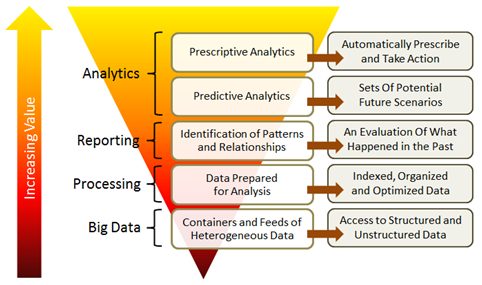
\includegraphics[width=\linewidth]{data-analytics.png}
%	\caption{Data analytics levels}
%	\label{fig:data-analytics}
%\end{figure}
%
%The basic idea is: provenance ontologies are used in software tools capturing provenance and reproducing the process of a certain task such as data preparation, so to evaluate the usability of such ontologies, we look at the complexity of software tools built on them. The less complex the software, the more usable the ontology.
%
%\begin{itemize}
%\item $\eta_1 = $Number of distinct operators.
%\item $\eta_2 = $Number of distinct operands.
%\item $N_1 = $Total number of operators.
%\item $N_2 = $Total number of operands.
%\end{itemize}
%%The program volume is defined to be
%%\begin{equation}
%%V = (N_1+N_2) \log_2(\eta_1+\eta_2).
%%\end{equation}
%An approximate formula for programming effort as a measure of program complexity is:
%\begin{equation}
%E = \frac{\eta_1N_2(N_1+N_2)\log_2(\eta_1+\eta_2)}{2\eta_2}.
%\end{equation}
%
%We choose the Halstead measure because the comparison of programming on top of different ontologies is mostly about the number and types of operations, rather than data flows (e.g., Oviedo in \cite{oviedo1993control} proposed a measure based on program data flows).
%
%We draw our data preparing operations from the R programming language. The assumption is that R is a data processing oriented programming language and the operations covered by R are typical for data processing.
%
%So the operations we are looking at are:
%\begin{itemize}
%	\item importing data from a file (be it a text file, an Excel spreadsheet, an XML file, or a netCDF file),
%	\item webscraping,
%	\item annotating datasets,
%	\item combining objects into a vector,
%	\item combining objects as columns or rows.
%\end{itemize}
%
%Currently we are picking typical data preparation tasks and describing them as combinations of the operations mentioned above. The plan is to calculate Halstead complexity values for programs based on PROV-PUB-O and directly on PROV-O for each hypothesis listed in the previous subsection to validate it.
%
%We originally planned to also describe the automatic provenance capturing mechanism and the proof-of-concept platform in this chapter. But the PROV-PUB-O part expands unexpectedly well and we decided to focus on it and move the other two sections to the future work chapter.

%\resetfootnote %this command starts footnote numbering with 1 again.

%\begin{figure}
%\centering
%\vspace{2.0in}
%\caption[A Shorter Caption for the List of Figures]
%   {This is the Caption for the First Figure in Chapter 2.  It is a
%    long, long caption; we do not want to put the whole thing in the
%    List of Figures. A Shorter Caption can go in the square brackets.}
% If you like additional lines in the caption indented, see the root template
% file rpithes.tex for an example of using the caption package to do this.
%\end{figure}
 
%This is shown in table~\ref{mytable}.  % see \label below
 
%\begin{table}
%\caption{This is the Caption for Table 2}
%\label{mytable}        % \label command must always comes AFTER the caption
%\begin{center}
%\begin{tabular}{lll}
%Here's       & another     & example  \\
%of           & a           & table    \\
%floated      & with        & the      \\
%\verb+table+ & environment & command.
%\end{tabular}
%\end{center}
%\end{table}


%\section{This is a Section Heading}
 
%\subsection{This is a Subsection Heading} 
 
%Text before a footnote.\footnote{Here's the text of the footnote.}
%Text after the footnote.


%%% Local Variables: 
%%% mode: latex
%%% TeX-master: t
%%% End: 
 % research approach
%%%%%%%%%%%%%%%%%%%%%%%%%%%%%%%%%%%%%%%%%%%%%%%%%%%%%%%%%%%%%%%%%%% 
%                                                                 %
%                           RELATED WORK                          %
%                                                                 %
%%%%%%%%%%%%%%%%%%%%%%%%%%%%%%%%%%%%%%%%%%%%%%%%%%%%%%%%%%%%%%%%%%% 

\chapter{RELATED WORK}
\label{related-work}
%\resetfootnote %this command starts footnote numbering with 1 again.

\section{General discussions on provenance and research reproducibility}
\label{sec:reproducibility}
%Jarvis in \cite{jarvis2010importance} talks about the importance of provenance in the context of journalism. 
%according to Tan et al \cite{tan2007provenance}, the provenance information discussed in this proposal falls into the category of workflow (or coarse-grained) provenance, where detailed transformation processes of specific pieces of data in the final publications are not captured. For example, the process of generating a table is captured, but not the process that leads to specific columns, rows or cells of the table, which includes data transformation details such as the aggregation function used and the deletion of outliers.

Donoho et al. in \cite{donoho2009reproducible} pointed out that current computational science practice, unlike the well-established deductive science and empirical science, doesn't generate routinely verifiable knowledge due to the lack of mature responses to the ubiquity of error in science such as formal logic and mathematical proof for deduction, and statistical hypothesis testing and standardized reproducibility information for empiricism. Following Claerbout's idea that
\begin{quote}\emph{
	We publish not just computational results
	but also the complete software environment
	and data that generated those results
}
\end{quote}
Donoho et al. developed the Wavelab package which contained a unified set of wavelet and time-frequency tools that reproduce all the calculations in the papers Donoho and his collaborators had written on computational harmonic analysis \cite{buckheit1995wavelab}. In \cite{donoho2009reproducible}, the authors mentioned that reproducible publication packages benefit \emph{strangers} who don't possess our current short-term memory and experiences.
\begin{quote}\emph{
	In the heat
	of a computational project, we store many things
	in short-term memory that we need at that moment
	to use the code productively.}
\end{quote}
In other words, conducting research in a reproducible manner hurts productivity in the heat of a project, although years from now, we ourselves, not remembering the myriad small details that accumulated in our minds during the very project of our own, will become such strangers.

Gentleman and Lang in \cite{gentleman2007statistical} proposed the idea of a \emph{research compendium}. A compendium can include several \emph{dynamic documents} that are mixtures of text and code. They also implemented a prototype by using a modified version of the \texttt{noweb} markup \cite{ramsey1994literate} to write dynamic documents, writing text chunks in a modified version of \LaTeX and writing code in R. Dynamic documents are processed with Sweave \cite{leisch2002sweave} and compendiums are represented as R packages.

Apparently, very few researchers have adopted the communication of research compendiums, as pointed out by Stodden in \cite{stodden2014enabling}. Most, if not all, of the problems listed in the \emph{Quick Answers to Knee-Jerk Objections} section of \cite{donoho2009reproducible} still remain in the way. For example, \emph{reproducibility takes time and effort}, although it may save us time in the long run. \emph{No one else does it, so I won't get any credit for it.} Creating compendiums instead of just papers really look wasting at the first sight. The list of problems goes on and on, and the consequences of not working reproducibly are serious despite the fact that it is somewhat hard to work in this way. In her talk in 2011 \cite{stodden2011establishing}, Stodden argued that the lack of transparency is hurting the credibility of scientific research based on her observation in the field of statistics. Further evidence comes from the field of biomedical research, where Bustin in \cite{bustin2015reproducibility} pointed out that there is increasing concern about the reliability of biomedical research. Bustin estimated that up to 85\% of research funding is wasted in unreliable research.

This thesis pursues the goal to reduce the time and effort required to create reproducible research publications. That is, the provenance capturing framework to be specified in Section~\ref{sec:framework} is for researchers who are willing to create reproducible publications but lack the knowledge and time to capture the necessary provenance.


%We plan to look further into the facts and references mentioned in this survey paper after proposal.

%The comment article introduces the series and discusses the consistent and colossal failure of initially promising research findings to translate into improvements in health care because of the many economic, political, social and cultural factors that influence researchers, funders, regulators, institutions and companies \cite{macleod2014biomedical}. 
%The first article in the series pointed out that the research studies supported by around US\$240 billion worldwide investment may have problems at the time funders decide what research to support, causing that much research does not lead to worthwhile achievements and that good research ideas do not yield the anticipated results \cite{chalmers2014increase}. 
%The second article in the series highlights that an absence of detailed written protocols and poor documentation of research is common and that inadequate emphasis is placed on recording of research decisions and on reproducibility of research \cite{ioannidis2014increasing}. 
%The third article discusses the modern approach to the regulation, governance, and management of biomedical research and emphasizes how inefficient management can easily compromise the interests of patients and the public \cite{salman2014increasing}. 
%The fourth article points out that a large percentage of protocols, reports and datasets associated with health research are rarely available, and there is selective reporting of methods and results, which leads to the introduction of bias and wastes huge amounts of research funding \cite{chan2014increasing}. The final article reemphasizes the absolute requirements for accurate, exhaustive and transparent reporting and notes that although reporting guidelines are important, they are all much less adopted and adhered to than they should be \cite{glasziou2014reducing}. The editors of the series make the revolutionary suggestion that rather than using journal impact factors to assess academics, it might be more reasonable to judge the researchers' work with the rigorousness of methodology, the transparency of reporting and the reproducibility of results, which would of course facilitate the publication of more reliable and biologically relevant data.


\section{Provenance models for research publications}
\subsection{Models for publication structure}
One important work on research publication structure modeling is the Document Components Ontology (DoCO), which is based on the rhetorical structure theory covered in \cite{taboada2006rhetorical}. This ontology integrated the SALT \cite{groza2007salt} (semantically annotates \LaTeX \ source files) ontology so that roles played by each part of the publication are made explicit. However, these roles are modeled as classes, which is against the fact that a role represents a relation between two entities. In the provenance ontology presented in this thesis, such roles are defined as properties to fit their relational nature, as will be described in Section~\ref{subsec:structure}.

Another model which is actively being developed now is nanopublications first proposed by Mons and Velterop~\cite{mons2009nano}. In this model, a nanopublication has three basic elements:
\begin{itemize}
	\item an assertion consisting of a subject, a predicate and an object,
	\item metadata providing contextual information about the assertion, and
	\item the publication information that is the metadata about the whole nanopublication.
\end{itemize}

The micropublications model proposed by Clark, Ciccarese and Goble in \cite{clark2013micropublications} extended statement-based models such as nano-publication by entities backing statements such as evidence and methods. In this model, a \emph{micropublication} argues \emph{claims}, which are supported by \emph{data}, other claims and \emph{attributions}, and data are produced by \emph{methods}.

The goal of our model for publication structure is to provide a way to describe and locate a published result in the context of a research publication, where \emph{results} could be in the form of figures, tables, lists and textual descriptions. We are more concerned about ``which section/chapter a certain figure is in'' than ``which statements support this claim'', so the abstract publication models such as nanopublications and micropublications do not fit our needs, while concrete models such as DoCO could serve well as a starting point to base our work.

%: a semantic model for claims, evidence, arguments and annotations in biomedical communications.

%And more to come after proposal...

\subsection{Models for publication preparing process}
Although no models have so far specifically been designed for the generation process of published results, there are models for locating and tracking provenance for general information. The example is Proof Markup Language version 2 (PML 2)~\cite{mcguinness2007pml}, of which the PML-P part (the provenance ontology of PML 2) models the concepts of \emph{information} and information container named \emph{source}. The ontology uses a ``raw string'' property to describe information content to deal with the heterogeneity of information, along with optional annotations such as ``language'', ``format'' and ``reference source usage'' (meaning how the information is obtained from a source). The process leading to some information is modeled in the PML-J part (the justification ontology of PML 2) as inference steps generating conclusions based on antecedent conclusions and rules applied by inference engines. The model fits the scenario of semantic web agents drawing conclusions with rules, but is counter-intuitive for modeling data and results generated by operations.

Moreau et al. in \cite{moreau2011open} presented the Open Provenance Model (OPM), which provides a digital representation of provenance in terms of \emph{artifacts}, \emph{processes} and \emph{agents}. An OPM provenance graph contains facts of artifacts being generated by processes, which used (other) artifacts and was controlled by agents. Artifacts, processes and agents, along with their associated \emph{edges}, could belong to \emph{accounts} so that each account owns a subgraph that is a view of the whole provenance graph. The purpose of the OPM ontology (OPMO, and its successor PROV-O) is to represent provenance for any ``thing'', whether produced by computer systems or not. Therefore, this kind of general ontologies are good fits to base our work of modeling research publication result provenance on.

The W3C Provenance ontology PROV-O\footnote{\url{http://www.w3.org/TR/prov-o/}, accessed on December 3rd, 2015.} shares a lot of elements with the OPM ontology\footnote{\url{http://openprovenance.org/model/opmo}, accessed on December 3rd, 2015.}. PROV-O's \emph{entity}, \emph{activity} and \emph{agent} classes could find their matches \emph{artifact}, \emph{process} and \emph{agent} in the OPM ontology. Properties in PROV-O such as \emph{used} and \emph{was generated by} are modeled as \emph{edges} in OPMO and have the same names in the Open Provenance Model Vocabulary (OPMV, which is a lightweight version of OPMO). The \emph{used} and \emph{was generated by} (edge) classes in OPMO correspond to \emph{Usage} and \emph{Generation} classes in PROV-O. The major difference between PROV-O and OPMO+OPMV is that PROV-O replaced the edge class with the qualified classes and replaced properties associated with edge class instances with qualified properties. 

The W3C recommended PROV-O received wide adoption and efforts have been made to specialize it to fit a variety of domains and applications. Missier et al. proposed D-PROV~\cite{missier2013d} to record not only provenance coming from certain runs of processes (called \emph{retrospective provenance}, or \emph{r-prov}), but also representation of these processes themselves (called \emph{perspective provenance}, or \emph{p-prov}). The D-PROV model is specially tailored for workflow systems, and defines both port-oriented and channel-oriented specializations of the \emph{was generated by} and \emph{used} properties in PROV-O to record r-prov. For example, data \emph{d} was observed on any output port of task invocation \emph{tInv} is a special case of ``data \emph{d} was generated by task invocation \emph{tInv}'',  and data \emph{d} was read from any channel by task invocation \emph{tInv} is a special case of ``task invocation \emph{tInv} used data \emph{d}''. Workflow and task representations are modeled as \emph{plans} to record p-prov. Our model, PROV-PUB-O, recognizes common usage patterns during the generation of published results to define sub-properties of \emph{used} and does not define any sub-properties for the \emph{was generated by} property in PROV-O. For p-prov, we introduced \emph{code} and (programming) \emph{language} properties for activities as shortcuts for their qualified associations' plans. Our model is specially tailored for processes that are representable with simple scripts coordinating library function invocations but does not conflict with plan-based embedding approaches to recording p-prov.

Costa et al. in \cite{costa2013capturing} presented another specialization of the PROV model for scientific workflows called \emph{PROV-Wf}. The model defined \emph{scientist} and \emph{machine} as two subclasses of \emph{agent} in PROV, \emph{workflow} and its composing tasks named \emph{WActivity} are defined as subclasses of \emph{plan}. Executions of these two plans, called \emph{execute workflow} and \emph{execute activity}, are defined as two subclasses of \emph{activity}. Inputs and outputs of workflow components are modeled as \emph{relation} whose schema can be defined with multiple \emph{fields}, each having a set of \emph{values}.

ProvONE\footnote{The ProvONE ontology. Available at \url{http://purl.dataone.org/provone-v1-dev}, accessed on November 18th, 2015.} integrated the work of Missier et al.'s D-PROV, Costa et al.'s PROV-Wf and Belhajjame et al.'s wfdesc ontology\footnote{The workflow description part of the Wf4ever Research Object Model. Available at \url{http://wf4ever.github.io/ro/#wfdesc}, accessed on November 23rd, 2015}. Although workflows are modeled as a type of programs, the ProvONE ontology uses workflow terms such as \emph{ports} and \emph{channels} to describe programs, so the scientific workflow community is likely to adopt the conceptualization of ProvONE quite readily. Figure~\ref{fig:provone} shows the major concepts defined in the ProvONE ontology.
\begin{figure}
	\centering
	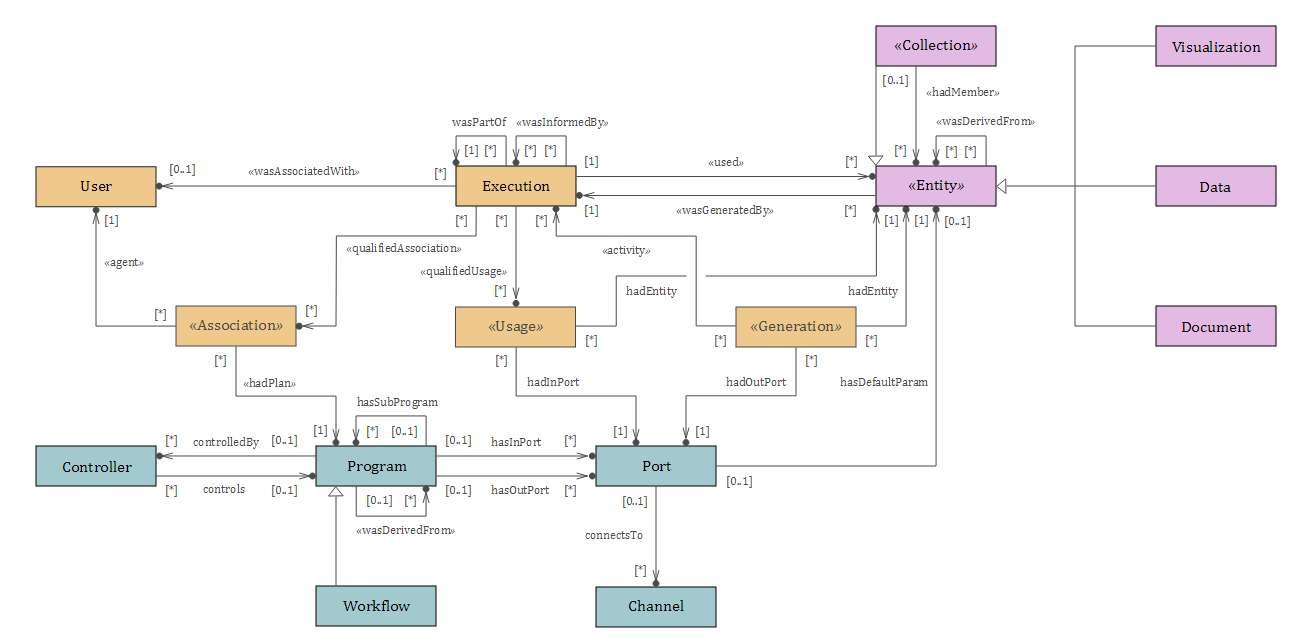
\includegraphics[width=\textwidth]{provone.png}
	\caption{ProvONE conceptual model UML diagram}
	\label{fig:provone}
\end{figure}
In ProvONE, the \emph{Program} class is a subclass of prov:Plan
Different from the ProvONE model, our model does not include specific concepts for workflows: it describes any operation implementable with scripts in a certain programming language with properties \emph{pub:language} and \emph{pub:code}, and any other operation with property \emph{dct:description}. Actually pub:DataGeneration and pub:ResultGeneration could be asserted as subclasses of provone:Execution so that provenance graphs in PROV-PUB-O and ProvONE are interoperable: in ProvONE, code could be found in the \emph{Program} objects of the prov:hadPlan property of the prov:qualifiedAssociation property of \emph{Execution} objects; in PROV-PUB-O, code is the pub:code property of \emph{DataGeneration/ResultGeneration} objects, which are also \emph{Execution} objects. 

Another interesting work, the \textit{Provenance, Authoring and Versioning} (PAV) ontology~\cite{ciccarese2013pav}, provided a lightweight vocabulary to capture the ``shallow'' provenance of a digital resource in terms of its relationships with other digital resources and agents. We call it ``shallow'' because the provenance information does not contain any activity details that tell how data are manipulated and/or transformed. The goal is to enrich related information of a digital resource, rather than to make it reproducible.
  
 %will be discussed in the final thesis.
%Zhao et al.~\cite{zhao2006applying} about prospective and retrospective provenance

%Freire et al.~\cite{freire2006managing} about process provenance or workflow evolution

\section{Ontology usability evaluation}
Ontology usability evaluation is related to the work of this thesis because we designed a set of ontology usability metrics to evaluate the provenance ontology created for research publications (See Section~\ref{subsec:evaluation} for details). To the best of our knowledge, we are the first to create such usability metrics for ontologies.

Ontology usability evaluation is an aspect of the more general task of ontology evaluation, which starts with checking completeness, consistency and conciseness of ontologies (e.g., \cite{gruninger1995methodology} and \cite{gomez2001evaluation}), so called \emph{deductive approaches} by Brank et al. in \cite{brank2005survey}.

To select an existing ontology to reuse in a new application, \emph{multiple-criteria approaches} (named by Brank et al. in \cite{brank2005survey}) were developed. Ontologies are evaluated by several criteria and scores are given per criteria. An overall score of the ontology then could be calculated as the weighted sum of per-criteria scores. For example, Lozano-Tello et al. presented the \emph{ONTOMETRIC} method in \cite{lozano2003selection,lozano2004ontometric}, which evaluates ontologies with a taxonomy of
160 characteristics organized in a multilevel framework. At the top level, there are five basic aspects. These are: 
\begin{itemize}
	\item the \emph{content} of the ontology and the
	organization of their contents,
	\item the \emph{language}
	in which it is implemented, 
	\item the \emph{methodology}
	that has been followed to develop it,
	\item the software \emph{tools} used to build and edit
	the ontology, and 
	\item the \emph{costs} that the ontology
	will be necessary in a certain project.
\end{itemize} 
As mentioned by Hartmann et al. in \cite{hartmann2005d1}, this method requires a substantial amount of time to specify the relevant criteria and the scores are given quite subjectively.

Burton-Jones et al. proposed an objective metric in \cite{burton2005semiotic}, where a set of 10 objective metrics at 4 different levels of a semiotic framework was presented. For example, at the \emph{syntactic} level, \emph{lawfulness} is defined as the total number of breached rules divided by the number of statements in the ontology, and \emph{richness} as the total number of syntactic features used in the ontology divided by the total number of available features in the ontology language. See Table 4 in \cite{burton2005semiotic} for the details of all the metrics. Since all the metrics used are objective, this approach does not require experts' review of the ontologies. However, the evaluation only gives the general quality of the ontology, which may have nothing to do with how well the ontology fits a certain task.

A really interesting work, although still not able to answer the ``how well it fits'' question, is \cite{gangemi2006qood}, where Gangemi et al. organized the criteria for ontology evaluation and selection with a semiotic meta-ontology called $O^2$ and the \emph{oQual} evaluation ontology which involves concepts and relations relevant to ontology evaluation and selection. Therefore, evaluation based on the oQual ontology goes beyond the mere calculation of a weighted sum, but also contains reasoning based on the evaluation ontology. For example, the two criteria, namely \emph{explicitness} and \emph{computational efficiency} could be detected as conflicting by this approach because the former goal indicates high rate of cycles in the ontology but the latter indicates low rate of cycles. (See Figure 4 in \cite{gangemi2006qood} for the details.) Such a reasoning mechanism sheds more light than mere scores on the trade-offs to consider for the selection of ontologies.

The few research efforts dealing with ontology usability evaluation includes \cite{casellas2009ontology}, which used System Usability Scale \cite{brooke1996sus} to evaluate the usability of the Ontology of Professional Judicial Knowledge (See Chapter 2 of \cite{casellas2009ontology} for a good introduction of the ontology).

\section{Provenance capturing approaches}
Groth and Moreau in \cite{groth2009recording} presented five characteristics of high quality process documentation (that is, the provenance information) for results produced by distributed systems, namely \emph{immutable}, meaning intact after creation, \emph{attributable}, meaning clear responsibility, \emph{autonomously creatable}, meaning created by the most appropriate agent, \emph{finalizable}, meaning clear timing of completeness, and \emph{process reflecting}, meaning able to reflect the whole process leading to the final product. They also presented the concept of p-assertions first defined in their earlier work with others \cite{groth2006architecture} and the six key actors in provenance-aware systems, namely application, sender, receiver, asserter, recorder and provenance store. They described PReP --- the P-assertion Recording Protocol based on these actors and the model of applications as actors communicating via message passing. Groth and Moreau's approach is specially tailored for distributed computing scenarios, where the actor model proposed by Agha et al.~\cite{agha1985actors,agha1997foundation} fits quite well. The framework specification of this thesis (see Section~\ref{sec:framework}) is based on the simple model of an application as a sequence of operation invocations carried out by operators. Our proof-of-concept prototype (to be described in Section~\ref{sec:prototype}) and case study (see Chapter~\ref{ch:case-study} for details) shows it is sufficient for research publication result preparation.

Miles et al. in \cite{miles2011prime} presents a provenance question driven methodology for developing provenance aware applications. The methodology decomposes the development process into three phases:
\begin{itemize}
	\item The \emph{use case identification} phase where provenance related requirements of the application are specified in terms of provenance questions and data items.
	\item The \emph{application decomposition} phase where the application is modeled in terms of actors and their interactions.
	\item The \emph{application adaptation} phase where the provenance capturing functions are engineered into the application.
\end{itemize}
The application is assumed to fit in the actor model, and the provenance captured is about interactions and actor state changes. We agree with Miles et al. that knowledgeable operators/actors, instead of a central provenance manager, are responsible for provenance capturing, so it is a reasonable approach to adapt normal programs used by researchers to capture provenance about executions of these programs themselves. Discussion about the responsible operators of provenance is in Section~\ref{sec:framework}, and a sample adaptation of several frequently used research programs is presented in Section~\ref{sec:prototype} and the source code is listed in Appendix~\ref{ap:prototype}.

Workflow systems such as VisTrails \cite{freire2014reproducibility}, Kepler \cite{ludascher2006scientific}, Taverna \cite{wolstencroft2013taverna} and ReproZip \cite{chirigati2013reprozip} represent software components able to create data artifacts as \emph{program} nodes with input and output \emph{ports} connected with each other through \emph{channels}, as summarized in the ProvONE ontology\footnote{The ProvONE ontology. Available at http://purl.dataone.org/provone-v1-dev, accessed on November 18th, 2015.}. These systems allow reuse of workflows as long as the users are using the same system as the workflow creator. The provenance of a particular data artifact would be the specific \emph{execution} sequence of a set of programs. Program nodes in workflows are unified in terms of input and output ports so that they are more ready to get reused than normal programs. A workflow actually represents program components in a more intuitive way than a set of programs in the form of source code/binary files. Data provenance is a by-product rather than the major focus. Workflow creators typically only record program execution related information and are limited on the additional information to add to the provenance graph.

%We also plan to look at the Severity Ratings for Usability Problems\footnote{http://www.nngroup.com/articles/how-to-rate-the-severity-of-usability-problems/ [Retrieved April 12th, 2015]}

%The approach we propose to develop is based on the intuition that better ontologies enable simpler software to accomplish a certain task, so we could evaluate the usability of ontologies by looking at the complexity of necessary software based on them.
%%% Local Variables: 
%%% mode: latex
%%% TeX-master: t
%%% End: 
 % related work
%%%%%%%%%%%%%%%%%%%%%%%%%%%%%%%%%%%%%%%%%%%%%%%%%%%%%%%%%%%%%%%%%%% 
%                                                                 %
%                            CHAPTER TWO                          %
%                                                                 %
%%%%%%%%%%%%%%%%%%%%%%%%%%%%%%%%%%%%%%%%%%%%%%%%%%%%%%%%%%%%%%%%%%% 
 
\chapter{DISCUSSIONS AND CONCLUSIONS}
%\resetfootnote %this command starts footnote numbering with 1 again.
This is a sentence to take up space and look like text.
This is a sentence to take up space and look like text.
 
This is a sentence to take up space and look like text.
This is a sentence to take up space and look like text.

\begin{figure}
\centering
\vspace{2.0in}
\caption[A Shorter Caption for the List of Figures]
   {This is the Caption for the First Figure in Chapter 2.  It is a
    long, long caption; we do not want to put the whole thing in the
    List of Figures. A Shorter Caption can go in the square brackets.}
% If you like additional lines in the caption indented, see the root template
% file rpithes.tex for an example of using the caption package to do this.
\end{figure}
 
This is a sentence to take up space and look like text.
This is a sentence to take up space and look like text.
This is a sentence to take up space and look like text.

This is shown in table~\ref{mytable}.  % see \label below
 
\begin{table}
\caption{This is the Caption for Table 2}
\label{mytable}        % \label command must always comes AFTER the caption
\begin{center}
\begin{tabular}{lll}
Here's       & another     & example  \\
of           & a           & table    \\
floated      & with        & the      \\
\verb+table+ & environment & command.
\end{tabular}
\end{center}
\end{table}
 
This is a sentence to take up space and look like text.
This is a sentence to take up space and look like text.
 
\section{This is a Section Heading}
 
This is a sentence to take up space and look like text.
This is a sentence to take up space \cite{Freire2014}.
This is a sentence to take up space and look like text.
This is a sentence to take up space and look like text.
 
\subsection{This is a Subsection Heading} 
 
This is a sentence to take up space and look like text.
This is a sentence to take up space and look like text.
This is a sentence to take up space and look like text.
Text before a footnote.\footnote{Here's the text 
of the footnote.}
Text after the footnote.
 
This is a sentence to take up space and look like text.
This is a sentence to take up space and look like text.
Text before another footnote.\footnote{Here's the 
text of the footnote.}
Text after the footnote.
This is a sentence to take up space and look like text.

%%% Local Variables: 
%%% mode: latex
%%% TeX-master: t
%%% End: 
 % discussions and conclusions
\chapter{FUTURE WORK}
\label{future-work}
\section{Workflow vs. provenance semantics}
Provenance is always about something that indeed \emph{happened}, i.e., not about something that \emph{is happening}, {\emph{will happen} or \emph{may happen}. Workflow is different, however, that it may contain conditional branches to express control logics such as \emph{if \dots then \dots else \dots} Therefore, it is important that we keep our mind clear on the semantic differences between provenance and workflow. Especially for provenance ontologies aiming at describing the details of the workflow leading to the data product in question. We plan to perform detailed checks on semantics of the proposed provenance ontology.

\section{Executable provenance graphs}
One reason we need to pay special attention to the semantic subtlety between provenance and workflow is that the proposed ontology will be able to define provenance graphs that are detailed enough to \emph{run} just like workflows. It is envisioned that such executable provenance graphs would be driven by standard RDF/OWL reasoners. We believe this approach to reproducibility has advantages over existing workflow systems in terms of implementability, maintainability and extensibility. We will compare the two approaches in detail in the final thesis.

\section{Ontology as software}
The comparison between workflow systems and executable provenance graphs inspire us that there might be more ways to ``put part of software into ontologies'', i.e., to transfer logics that would otherwise written with programming languages to ontologies. In this sense, ontologies could be seen as transparent software with logics explicitly and formally described. We hope we could find interesting insights on this topic in the final thesis.

\section{Automatic provenance capturing mechanism}
This topic is originally a task with the same weight as ``creating a provenance capturing ontology''. But the ontology topic expands unexpectedly well and we decided to focus on it and put the provenance capturing mechanism as a future work. The mechanism is designed to make provenance capturing chores less distracting for the authors. As mentioned in Section \ref{sec:reproducibility}, Donoho et al admitted that recording provenance hurts productivity, although in the long run its benefits would way supersede its shortcomings. We believe it is possible to overcome the short-term counter-productive weakness of working reproducibly by using authoring tools that transparently record provenance for the authors. As mentioned in Section \ref{sec:possibility}, we will try to develop provenance aware tools with the same or similar user interfaces with existing tools to save learning time for researchers, and these tools save provenance in the background so they do not require explicit effort of recording provenance from the authors.

%\comment{Compare Groth's architecture with the proposed mechanism}

\section{A proof-of-concept platform}
A natural follow-up of the automatic provenance capturing mechanism is to develop a proof-of-concept platform that demonstrates the desired features of provenance aware authoring tools. As mentioned in Section \ref{sec:contribution}, we are looking for a portable and function-rich implementation with user-familiar interfaces.

%Hypotheses:

%3: The implemented platform satisfies the requirements indicated by the mechanism.

%3.1: The platform does not require explicit input from authors to capture provenance for research publications.

%3.2: The platform is more useful than workflow systems for carrying out operations in research publication preparation process.

%3.3: The platform captures sufficient provenance for replicating research publications.


%%% Local Variables: 
%%% mode: latex
%%% TeX-master: t
%%% End: 
 % future work
%%%%%%%%%%%%%%%%%%%%%%%%%%%%%%%%%%%%%%%%%%%%%%%%%%%%%%%%%%%%%%%%%%% 
%                                                                 %
%                           BIBLIOGRAPHY                          %
%                                                                 %
%%%%%%%%%%%%%%%%%%%%%%%%%%%%%%%%%%%%%%%%%%%%%%%%%%%%%%%%%%%%%%%%%%% 
 
%This method produces a numbered bibliography where the numbers
%correspond to the \cite commands in the text. See the LaTeX manual.
%
\specialhead{REFERENCES}
\bibliographystyle{alpha}
\begin{singlespace}
\bibliography{refs}
\end{singlespace}

% Note that, if you wish, you can use BibTeX to create your bibliography
% from a database. See section 5.6.2 of Memo RPI.110 for information. 
%%% Local Variables: 
%%% mode: latex
%%% TeX-master: t
%%% End: 
 % bibliography
%%%%%%%%%%%%%%%%%%%%%%%%%%%%%%%%%%%%%%%%%%%%%%%%%%%%%%%%%%%%%%%%%%%%
%                                                                 %
%                            APPENDICES                           %
%                                                                 %
%%%%%%%%%%%%%%%%%%%%%%%%%%%%%%%%%%%%%%%%%%%%%%%%%%%%%%%%%%%%%%%%%%%
 
\appendix    % This command is used only once!
%\addcontentsline{toc}{chapter}{APPENDICES}             %toc entry  or:
\addtocontents{toc}{\parindent0pt\vskip12pt APPENDICES} %toc entry, no page #

\chapter{PROV-PUB-O/S serialized in Turtle (TTL)}
\lstinputlisting{model/prov-pub-s4listing.ttl}

\section{A Section Heading}

This is how equations are numbered in an appendix:
\begin{equation}
x^2 + y^2 = z^2
\end{equation} 
This is a sentence to take up space and look like text.
This is a sentence to take up space and look like text.
This is a sentence to take up space and look like text.
 
This is a sentence to take up space and look like text.
This is a sentence to take up space and look like text.
This is a sentence to take up space and look like text.
This is a sentence to take up space and look like text.
This is a sentence to take up space and look like text. 

\chapter{THIS IS ANOTHER APPENDIX} 
This is a sentence to take up space and look like text.
This is a sentence to take up space and look like text.
This is a sentence to take up space and look like text.
This is a sentence to take up space and look like text.
This is a sentence to take up space and look like text.
This is a sentence to take up space and look like text.
This is a sentence to take up space and look like text.
This is a sentence to take up space and look like text.
 
 % appendix

\end{document}
